\section{Appendix}

Everything in this appendix is generated from \texttt{results/} by \texttt{code/make\_report\_appendix.py}, so the tables cannot drift from the artefacts submitted with the code. The course guideline exempts appendices from the seven-page limit on the body.

\begin{table}[!htbp]
  \caption{Variables in the cleaned data set: 29 predictors and the target, 29,965 clients after removing 35 exact duplicate rows.}
  \label{tab:a-variables}
  \centering
  \small
  \begin{tabular}{@{}L{0.14\linewidth}L{0.25\linewidth}L{0.12\linewidth}L{0.35\linewidth}@{}}
    \toprule
    Group & Variables & Type & Meaning \\
    \midrule
    Credit line & \texttt{LIMIT\_\allowbreak{}BAL} & numeric & credit limit granted (NT\$), individual plus family \\
    Demographics & \texttt{SEX},\allowbreak\ \texttt{EDUCATION},\allowbreak\ \texttt{MARRIAGE},\allowbreak\ \texttt{AGE} & 3 categorical, 1 numeric & gender; graduate / university / high school / others; married / single / others; age in years \\
    Repayment status & \texttt{PAY\_\allowbreak{}1},\allowbreak\ \dots,\allowbreak\ \texttt{PAY\_\allowbreak{}6} & ordinal ($-2 \dots 8$) & monthly status Sep $\rightarrow$ Apr 2005: $-2$ no consumption, $-1$ paid in full, $0$ revolving credit, $k \ge 1$ = $k$ months of delay \\
    Bill statements & \texttt{BILL\_\allowbreak{}AMT1},\allowbreak\ \dots,\allowbreak\ \texttt{BILL\_\allowbreak{}AMT6} & numeric & monthly bill amount Sep $\rightarrow$ Apr (NT\$); may be negative \\
    Payments & \texttt{PAY\_\allowbreak{}AMT1},\allowbreak\ \dots,\allowbreak\ \texttt{PAY\_\allowbreak{}AMT6} & numeric & amount paid in each month Sep $\rightarrow$ Apr (NT\$) \\
    Engineered & \texttt{UTIL\_\allowbreak{}1},\allowbreak\ \texttt{UTIL\_\allowbreak{}MEAN},\allowbreak\ \texttt{PAY\_\allowbreak{}RATIO\_\allowbreak{}MEAN},\allowbreak\ \texttt{N\_\allowbreak{}MONTHS\_\allowbreak{}DELAYED},\allowbreak\ \texttt{MAX\_\allowbreak{}DELAY},\allowbreak\ \texttt{BILL\_\allowbreak{}TREND} & numeric & utilisation of the limit (latest, mean); mean payment-to-bill ratio; months in arrears; worst delay; six-month balance trend relative to the limit \\
    Target & \texttt{DEFAULT} & binary & 1 = default on the October 2005 payment (22.1\% in training) \\
    \bottomrule
  \end{tabular}
\end{table}

\begin{table}[!htbp]
  \caption{Default rate along the two strongest credit-risk gradients, training partition only ($n = 20,975$; overall rate 22.1\%). Source: \texttt{results/eda\_summary.json}.}
  \label{tab:a-gradients}
  \centering
  \small
  \begin{tabular}{@{}lrrlrr@{}}
    \toprule
    September status & Clients & Default & Credit-limit quintile & Clients & Default \\
    \midrule
    No consumption ($-2$) & 1,904 & 13.7\% & NT\$10k--50k & 5,429 & 32.0\% \\
    Paid in full ($-1$) & 3,941 & 16.9\% & NT\$50k--100k & 3,370 & 25.5\% \\
    Revolving credit (0) & 10,380 & 12.9\% & NT\$100k--180k & 4,224 & 19.5\% \\
    1 month late & 2,540 & 33.9\% & NT\$180k--270k & 3,810 & 17.1\% \\
    2 months late & 1,871 & 67.6\% & NT\$270k--1M & 4,142 & 13.7\% \\
    3 months late & 234 & 77.3\% &  &  &  \\
    \bottomrule
  \end{tabular}
\end{table}

\begin{table}[!htbp]
  \caption{Data-quality checks run on the raw download before modelling, and what was done about each finding. Reproduced verbatim from \texttt{results/eda\_data\_quality.csv}; the three cleaning steps that precede the split (duplicate removal, the fixed recoding of undocumented codes, the row-wise engineered features) estimate nothing from the data, and everything else is left to the in-fold pipeline.}
  \label{tab:a-quality}
  \centering
  \footnotesize
  \setlength{\tabcolsep}{3pt}
  \begin{tabular}{@{}L{0.19\linewidth}L{0.36\linewidth}L{0.39\linewidth}@{}}
    \toprule
    Check & Finding & Action \\
    \midrule
    Missing values & 0 cells (all 24 columns complete) & None needed — no imputation step in the pipeline \\
    Exact duplicate rows & 35 of 30,000 (0.12\%) & Dropped in common.clean() → 29,965 rows \\
    Data types & All 24 columns integer; no strings, no dates & --- \\
    EDUCATION undocumented codes 0/5/6 & 0: 14, 5: 280, 6: 51 (total 345, 1.15\%) & Recoded to 4 = others/unknown \\
    MARRIAGE undocumented code 0 & 54 rows (0.18\%) & Recoded to 3 = others \\
    PAY\_1..6 undocumented codes -2 and 0 & PAY\_1: -2 in 2,759 rows, 0 in 14,737 rows (codebook lists only -1 and 1..9) & Kept as ordinal: -2 = no consumption, -1 = paid in full, 0 = revolving credit / minimum paid, k>0 = k months late \\
    Negative bill amounts & 3,932 cells in 1,930 rows (6.4\%); min BILL\_AMT = -339,603 & Kept — a negative bill is a credit balance (overpayment / refund) \\
    Zero payments & PAY\_AMT = 0 in at least one month for 14,542 rows (48.5\%); all six months zero for 1,432 rows (4.8\%) & Kept — 'no payment' is informative; PAY\_RATIO\_MEAN handles zero bills \\
    Zero bills in all six months & 866 of the raw 30,000 rows (2.9\%); 936 of the 29,965 cleaned rows (3.12\%) have all six bills NON-POSITIVE & Kept — inactive or credit-balance accounts. For the non-positive group PAY\_RATIO\_MEAN is undefined and imputed 0; in the training partition that group defaults at 37.0\% against 21.7\% for the rest, so the imputed value is informative rather than neutral \\
    Bill above credit limit (UTIL\_1 > 1) & 2,115 rows (7.1\%); max UTIL\_1 = 6.46 & Kept — over-limit usage is a genuine risk signal \\
    LIMIT\_BAL range & 10,000 – 1,000,000 NT\$ (median 140,000) & Plausible; heavy right tail → StandardScaler inside the pipeline, no trimming \\
    AGE range & 21 – 79 years (median 34) & Plausible; no outlier removal \\
    Class imbalance & 6,630 defaults of 29,965 = 22.1\% & Kept as is; addressed downstream by class\_weight / threshold tuning; AUC \& AP as metrics \\
    Train / test split & 20,975 / 8,990 rows, stratified 70/30, seed 2607526; default rate 22.13\% / 22.12\% & Fixed once in data/processed; test set untouched in this EDA \\
    \bottomrule
  \end{tabular}
\end{table}

\begin{table}[!htbp]
  \caption{Contribution by section. Percentages are of the writing and analysis behind each section; the model families below are owned end to end --- data, tuning, interpretation and presentation --- by the member named. The percentages are the group's draft of 21 October 2026 and are typeset in red until all three members have confirmed them.}
  \label{tab:a-workload}
  \centering
  \small
  \begin{tabular}{@{}L{0.20\linewidth}cccL{0.34\linewidth}@{}}
    \toprule
    Section & RUAN & LU & LI & Basis \\
    \midrule
    Abstract, \S1 Introduction & \textcolor{red}{30\%} & \textcolor{red}{20\%} & \textcolor{red}{50\%} & LI drafted; RUAN and LU revised \\
    \S2 Data & \textcolor{red}{25\%} & \textcolor{red}{15\%} & \textcolor{red}{60\%} & LI wrote the cleaning and split contract and the exploratory analysis \\
    \S3 Methods & \textcolor{red}{30\%} & \textcolor{red}{25\%} & \textcolor{red}{45\%} & shared protocol; RUAN the nested cross-validation, LI the freeze and recalibration protocol \\
    \S4 Results & \textcolor{red}{30\%} & \textcolor{red}{35\%} & \textcolor{red}{35\%} & RUAN: KNN, logistic family, second pass; LU: tree, forest, GBM, XGBoost; LI: SVM, MLP, LDA/QDA/NB, imbalance study, aggregation and bootstrap \\
    \S5 Interpretation & \textcolor{red}{15\%} & \textcolor{red}{60\%} & \textcolor{red}{25\%} & LU owns TreeSHAP, the monotone constraints, partial dependence and the forest importances \\
    \S6 Choosing the operating point & \textcolor{red}{40\%} & \textcolor{red}{15\%} & \textcolor{red}{45\%} & RUAN: cost-ratio table and nested CV; LI: recalibration and threshold analysis \\
    \S7 Conclusion and limitations & \textcolor{red}{34\%} & \textcolor{red}{33\%} & \textcolor{red}{33\%} & drafted jointly \\
    Code and reproducibility & \textcolor{red}{20\%} & \textcolor{red}{25\%} & \textcolor{red}{55\%} & LI: \texttt{common.py}, aggregation, freeze, recalibration \\
    Presentation & \textcolor{red}{33\%} & \textcolor{red}{33\%} & \textcolor{red}{34\%} & three presenters, 10 minutes \\
    \bottomrule
  \end{tabular}
  \\[3pt]\begin{minipage}{\linewidth}\footnotesize Each model family is run end to end by its owner: \textbf{RUAN Hangjing} --- KNN benchmark; logistic family (plain, ridge, lasso, class-weighted); PCA and K-means; \textbf{LU Xinyu} --- Pruned tree; random forest and bagging; gradient boosting and XGBoost; TreeSHAP; monotone-constrained XGBoost; partial dependence; \textbf{LI Jingwen} --- Support-vector machines; feed-forward neural network; LDA, QDA and naive Bayes; class-imbalance study and the leakage demonstration. The owner of every file in \texttt{results/} is recorded in its \texttt{member} field, so this table is checkable against the submitted code. This project is not shared with any other module.\end{minipage}
\end{table}

\begin{table}[htbp]
  \caption{Model families, the lecture that introduces each one, and what each is in the study to test. The last three rows are beyond the syllabus.}
  \label{tab:a-methods}
  \centering
  \small
  \begin{tabular}{@{}L{0.30\linewidth}L{0.62\linewidth}@{}}
    \toprule
    Family (lecture) & What it is there to test \\
    \midrule
    PCA, K-means, hierarchical clustering (B2--B3) & Whether default risk lies along the directions of largest variance, and whether a segment label carries anything a supervised model has not already found. \\
    K-nearest neighbours (B4) & Benchmark: how much of the signal a scaled distance and a local default rate recover with no model of the risk at all. \\
    Class weights, SMOTE, under-sampling (B4) & Whether re-balancing changes the ordering of clients or only the prior behind it; and what resampling before the split fabricates. \\
    Logistic regression: plain, ridge, lasso (B5--B6) & Whether the ceiling on this data is variance, which shrinkage can cut, or the bias of a model linear in the features, which it cannot. \\
    LDA, QDA, naive Bayes (B6) & The price of distributional assumptions: a shared covariance, class-specific covariances on skewed amounts, and independence among near-collinear balances. \\
    Decision tree, cost-complexity pruning (B7) & The bias--variance trade-off made readable: delay thresholds and their interactions, bought at the cost of very few distinct scores. \\
    Random forest and bagging (B7) & Whether de-correlating trees, not merely averaging them, is what removes variance; out-of-bag error and permutation importance come free. \\
    Gradient boosting and XGBoost (B7) & Whether sequential bias reduction beats variance reduction on a noisy target, and how much of that depends on shrinkage. \\
    Support-vector machines, linear and RBF (B8) & Whether a margin loss that ignores ordering beyond the margin can rank risk as well as a proper scoring rule. \\
    Feed-forward neural network (B9) & Whether learned interactions help when the strongest predictors are ordinal delay codes with step-like effects. \\
    \midrule
    TreeSHAP (beyond the syllabus) & Direction and size of each variable's push on each individual client, rather than one global ranking; additive by construction, so it can be checked. \\
    Monotonically constrained XGBoost (beyond the syllabus) & The cost, in ranking quality, of the scorecard requirement that more arrears may never lower predicted risk. \\
    Partial dependence and ICE (beyond the syllabus) & Whether the fitted surface carries the U-shaped utilisation effect a linear term cannot express, and whether effects add or interact. \\
    \bottomrule
  \end{tabular}
\end{table}

\begin{table}[!htbp]
  \caption{Hyper-parameter grids searched for the headline models and the setting chosen, read from \texttt{results/<slug>.json}. Every grid is scored by 5-fold stratified cross-validation on the training partition (seed 2607526); the test set plays no part. The last column is the training-set selection score of the chosen setting (CV AUC; out-of-fold AUC for the subsample-tuned RBF SVM).}
  \label{tab:a-tuning}
  \centering
  \small
  \setlength{\tabcolsep}{3pt}
  \begin{tabular}{@{}L{0.15\linewidth}L{0.40\linewidth}L{0.29\linewidth}c@{}}
    \toprule
    Model & Grid searched & Chosen & Sel.\ AUC \\
    \midrule
    XGBoost & \texttt{max\_\allowbreak{}depth} \{3, 4, 6\} $\times$ \texttt{learning\_\allowbreak{}rate} \{0.03, 0.1\} $\times$ \texttt{n\_\allowbreak{}estimators} \{300, 600\} $\times$ \texttt{min\_\allowbreak{}child\_\allowbreak{}weight} \{5, 1\} (24 settings); \texttt{subsample} = 0.8, \texttt{colsample\_\allowbreak{}bytree} = 0.8 fixed; rounds then checked on a learning curve to 1500 & \texttt{max\_\allowbreak{}depth} = 3, \texttt{learning\_\allowbreak{}rate} = 0.03, \texttt{n\_\allowbreak{}estimators} = 300, \texttt{min\_\allowbreak{}child\_\allowbreak{}weight} = 5 & 0.7863 \\
    Gradient boosting (sklearn) & \texttt{learning\_\allowbreak{}rate} \{0.03, 0.1\} $\times$ \texttt{max\_\allowbreak{}depth} \{3, 2, 4\} $\times$ \texttt{n\_\allowbreak{}estimators} \{200, 500\} (12 settings) on a 10,487-row training subsample; staged CV curve on the full training set & \texttt{learning\_\allowbreak{}rate} = 0.03, \texttt{max\_\allowbreak{}depth} = 3, \texttt{n\_\allowbreak{}estimators} = 200, \texttt{subsample} = 0.8 & 0.7850 \\
    Random forest & \texttt{max\_\allowbreak{}features} \{sqrt, 0.3, 0.5\} $\times$ \texttt{min\_\allowbreak{}samples\_\allowbreak{}leaf} \{20, 5, 1\} (9 settings) at 200 trees; top two re-run at 500 trees & \texttt{max\_\allowbreak{}features} = sqrt, \texttt{min\_\allowbreak{}samples\_\allowbreak{}leaf} = 20, \texttt{n\_\allowbreak{}estimators} = 500 & 0.7849 \\
    MLP (feed-forward NN) & \texttt{hidden\_\allowbreak{}layer\_\allowbreak{}sizes} \{32, 64, 64x32, 128x64\} $\times$ \texttt{alpha} \{0.0001, 0.001, 0.01\} $\times$ \texttt{learning\_\allowbreak{}rate\_\allowbreak{}init} \{0.001, 0.003\} (24 settings); \texttt{relu}, \texttt{adam}, early stopping fixed & \texttt{hidden\_\allowbreak{}layer\_\allowbreak{}sizes} = 64x32, \texttt{alpha} = 0.001, \texttt{learning\_\allowbreak{}rate\_\allowbreak{}init} = 0.001 & 0.7762 \\
    KNN & \texttt{K} \{5 \dots\ 151\} (12 values) $\times$ \texttt{weights} \{uniform, distance\} (24 settings) & \texttt{n\_\allowbreak{}neighbors} = 101, \texttt{weights} = uniform & 0.7700 \\
    Decision tree (pruned) & \texttt{ccp\_\allowbreak{}alpha} \{0 \dots\ 0.02493\} (21 values) (cost-complexity path) $\times$ \texttt{max\_\allowbreak{}depth} \{None, 4, 6, 8\} & \texttt{criterion} = entropy, \texttt{ccp\_\allowbreak{}alpha} = 0.000663, \texttt{max\_\allowbreak{}depth} = 6 & 0.7689 \\
    SVM (RBF kernel) & \texttt{C} \{0.1, 1, 10\} $\times$ \texttt{gamma} \{scale, 0.01, 0.1\} $\times$ \texttt{class\_\allowbreak{}weight} \{None, balanced\} on a 6,000-row training subsample; one-standard-error rule & \texttt{C} = 1, \texttt{gamma} = 0.01, \texttt{class\_\allowbreak{}weight} = balanced; Platt-scaled & 0.7606 \\
    Logistic regression (plain) & none: unpenalised reference fit & \texttt{C} = inf (unpenalised), \texttt{solver} = lbfgs & 0.7602 \\
    Logistic regression (L1 lasso, C tuned) & \texttt{C} \{0.001 \dots\ 100\} (11 values) & \texttt{C} = 100, \texttt{penalty} = l1 (l1\_ratio=1) & 0.7602 \\
    LDA (linear discriminant analysis) & \texttt{shrinkage} \{None, auto, 0.05, 0.2, 0.5\} & \texttt{solver} = lsqr, \texttt{shrinkage} = None & 0.7572 \\
    Gaussian naive Bayes & \texttt{var\_\allowbreak{}smoothing} \{1e-09 \dots\ 0.1\} (9 values) & \texttt{var\_\allowbreak{}smoothing} = 0.01 & 0.7356 \\
    \bottomrule
  \end{tabular}
\end{table}

\begin{table}[!htbp]
  \caption{Software versions and the single seed behind every result in this report. Versions are the ones recorded in the result files by the scripts that produced them.}
  \label{tab:a-software}
  \centering
  \small
  \begin{tabular}{@{}L{0.42\linewidth}L{0.50\linewidth}@{}}
    \toprule
    Component & Version / value \\
    \midrule
    Python & 3.13.5 \\
    scikit-learn & 1.9.0 \\
    XGBoost & 3.4.1 \\
    SHAP & 0.52.0 \\
    NumPy & 2.5.1 \\
    pandas & 3.0.5 \\
    imbalanced-learn & 0.14.2 \\
    SciPy & 1.18.0 \\
    Random seed (split, folds, samplers, every model) & 2607526 \\
    Cross-validation & 5 stratified folds of the training partition, shuffled with the seed \\
    Split & stratified 70/30, 20,975 training / 8,990 test rows \\
    \bottomrule
  \end{tabular}
\end{table}
\clearpage

\begin{table}[!htbp]
  \caption{The monotone constraint vector of the constrained XGBoost, fixed a priori from credit logic and read back from the fitted booster: \texttt{(-1,\allowbreak 0,\allowbreak 1,\allowbreak 1,\allowbreak 1,\allowbreak 1,\allowbreak 1,\allowbreak 1,\allowbreak 0,\allowbreak 0,\allowbreak 0,\allowbreak 0,\allowbreak 0,\allowbreak 0,\allowbreak 0,\allowbreak 0,\allowbreak 0,\allowbreak 0,\allowbreak 0,\allowbreak 0,\allowbreak 1,\allowbreak 1,\allowbreak -1,\allowbreak 1,\allowbreak 1,\allowbreak 1,\allowbreak 0,\allowbreak 0,\allowbreak 0,\allowbreak 0,\allowbreak 0,\allowbreak 0)} over the 32 preprocessed columns (one-hot categories count once per raw variable here). Hyper-parameters are inherited unchanged from the tuned unconstrained model.}
  \label{tab:a-monotone}
  \centering
  \small
  \begin{tabular}{@{}L{0.30\linewidth}L{0.54\linewidth}c@{}}
    \toprule
    Sign & Variables & $n$ \\
    \midrule
    $+1$ (more may only raise the predicted risk) & \texttt{PAY\_\allowbreak{}1},\allowbreak\ \texttt{PAY\_\allowbreak{}2},\allowbreak\ \texttt{PAY\_\allowbreak{}3},\allowbreak\ \texttt{PAY\_\allowbreak{}4},\allowbreak\ \texttt{PAY\_\allowbreak{}5},\allowbreak\ \texttt{PAY\_\allowbreak{}6},\allowbreak\ \texttt{N\_\allowbreak{}MONTHS\_\allowbreak{}DELAYED},\allowbreak\ \texttt{MAX\_\allowbreak{}DELAY},\allowbreak\ \texttt{UTIL\_\allowbreak{}1},\allowbreak\ \texttt{UTIL\_\allowbreak{}MEAN},\allowbreak\ \texttt{BILL\_\allowbreak{}TREND} & 11 \\
    $-1$ (more may only lower it) & \texttt{LIMIT\_\allowbreak{}BAL},\allowbreak\ \texttt{PAY\_\allowbreak{}RATIO\_\allowbreak{}MEAN} & 2 \\
    $0$ (unconstrained) & \texttt{AGE},\allowbreak\ \texttt{BILL\_\allowbreak{}AMT1},\allowbreak\ \texttt{BILL\_\allowbreak{}AMT2},\allowbreak\ \texttt{BILL\_\allowbreak{}AMT3},\allowbreak\ \texttt{BILL\_\allowbreak{}AMT4},\allowbreak\ \texttt{BILL\_\allowbreak{}AMT5},\allowbreak\ \texttt{BILL\_\allowbreak{}AMT6},\allowbreak\ \texttt{PAY\_\allowbreak{}AMT1},\allowbreak\ \texttt{PAY\_\allowbreak{}AMT2},\allowbreak\ \texttt{PAY\_\allowbreak{}AMT3},\allowbreak\ \texttt{PAY\_\allowbreak{}AMT4},\allowbreak\ \texttt{PAY\_\allowbreak{}AMT5},\allowbreak\ \texttt{PAY\_\allowbreak{}AMT6},\allowbreak\ \texttt{SEX},\allowbreak\ \texttt{EDUCATION},\allowbreak\ \texttt{MARRIAGE} & 19 \\
    \bottomrule
  \end{tabular}
  \\[3pt]\begin{minipage}{\linewidth}\footnotesize Sweeping each constrained variable with the others at their training median, the unconstrained booster moves against the required direction on 24 grid steps in total (3 of them on \texttt{PAY\_1}); over 200 random training profiles it violates monotonicity in \texttt{PAY\_1} on 576 of 2,000 steps (largest fall 0.036); the constrained booster on none. Price of the constraint: CV AUC $-0.0019$, test AUC $-0.0016$ (paired bootstrap, $B=500$: mean $-0.0017$, 95\,\% interval [$-0.0030$, $-0.0002$]).\end{minipage}
\end{table}

\begin{table}[!htbp]
  \caption{Freeze timeline: the 46 entries of \texttt{results/frozen\_manifest.json} grouped by round. A configuration is frozen the first time it is scored on the test set, and \texttt{common.evaluate()} refuses to score a changed configuration under a frozen slug (\texttt{code/freeze.py -{}-check} verifies every stored prediction vector).}
  \label{tab:a-freeze}
  \centering
  \small
  \setlength{\tabcolsep}{3pt}
  \begin{tabular}{@{}cL{0.12\linewidth}cL{0.40\linewidth}L{0.26\linewidth}@{}}
    \toprule
    Round & Scored & $n$ & What & Selection basis \\
    \midrule
    1 & 16 Sep--18 Sep & 34 & every model variant of Table~\ref{tab:a-allmodels}: each configuration tuned on training CV, then scored on the test set once and frozen (before the professor's 30 September comment); none re-scored since & 5-fold CV AUC on the training partition; both thresholds on training out-of-fold probabilities \\
    2 & 30 Sep & 2 & RUAN Hangjing's second pass under her freeze-before-test protocol (\texttt{frozen\_choices\_ruan\_v2.json}): the KNN ($K=101$, uniform) and plain-logistic configurations re-fitted and re-scored; adopted on 21 October unchanged; the headline tables keep the round-1 scoring (predictions differ by $\le 10^{-2}$, test AUC by $5\times10^{-5}$) & nested CV with the pre-registered 1-SE and 1\,\% cost rules (Table~\ref{tab:a-nestedcv}); training rows only \\
    3 & 19 Oct & 9 & Platt-recalibrated versions of the nine class-weighted or resampled models (Table~\ref{tab:a-recal}), each scored once & Platt map fitted on training out-of-fold scores; thresholds re-chosen on cross-fitted training scores \\
    --- & 17 Sep & 1 & negative control: SMOTE applied before the split (the leakage demonstration); its `test' rows are not the real test set and it is not a model result & none --- deliberately leaky \\
    \bottomrule
  \end{tabular}
\end{table}

\begin{table}[!htbp]
  \caption{Nested cross-validation of the KNN and logistic families, RUAN Hangjing's second pass of 30 September 2026 (\texttt{logistic\_\allowbreak{}nested\_\allowbreak{}cv\_\allowbreak{}v2.csv}, \texttt{knn\_\allowbreak{}v2.json}). The 21 October reproduction on the training rows (\texttt{nested\_\allowbreak{}cv\_\allowbreak{}summary\_\allowbreak{}repro.json}, \texttt{logistic\_\allowbreak{}nested\_\allowbreak{}cv\_\allowbreak{}repro.csv}) matched the nested AUCs and standard errors, the logistic rows and the selected configurations; the KNN Brier and calibration-slope columns are RUAN's 30 September out-of-fold figures (\texttt{knn\_\allowbreak{}v2.json}), which the reproduction (\texttt{nested\_\allowbreak{}cv\_\allowbreak{}knn\_\allowbreak{}repro.json}) puts at 0.1395 and 0.966. The pre-registered rules re-select the configurations frozen on 16 September.}
  \label{tab:a-nestedcv}
  \centering
  \footnotesize
  \setlength{\tabcolsep}{3pt}
  \begin{tabular}{@{}L{0.30\linewidth}cccccc@{}}
    \toprule
    Model & Nested AUC & Nested AP & Brier & Cal.\ slope & 5:1 cut-off & 5:1 cost \\
    \midrule
    Logistic, plain (unpenalised) & 0.7602 $\pm$ 0.0050 & 0.5049 & 0.1410 & 0.982 & 0.17 & 12,195 \\
    Logistic, ridge ($C$ tuned inside each fold) & 0.7601 $\pm$ 0.0051 & 0.5049 & 0.1410 & 0.985 & 0.17 & 12,205 \\
    Logistic, lasso ($C$ tuned inside each fold) & 0.7602 $\pm$ 0.0050 & 0.5049 & 0.1410 & 0.982 & 0.15 & 12,188 \\
    Logistic, class-weighted & 0.7608 $\pm$ 0.0055 & 0.5020 & 0.1920 & 0.974 & 0.39 & 12,263 \\
    Logistic, class-weighted + Platt & 0.7608 $\pm$ 0.0055 & 0.5022 & 0.1412 & 1.004 & 0.15 & 12,247 \\
    KNN ($K$, weights tuned in-fold; $K=101$ uniform chosen) & 0.7684 $\pm$ 0.0073 & --- & 0.1392 & 0.989 & --- & --- \\
    \bottomrule
  \end{tabular}
  \\[3pt]\begin{minipage}{\linewidth}\footnotesize Nested CV: outer loop = the project's five folds, inner loop = a 5-fold grid search inside each outer training fold, so the AUC is that of the whole tuning procedure. Columns: nested AUC $\pm$ its standard error over the outer folds (for KNN, the standard deviation), nested average precision, Brier score and calibration slope of the nested out-of-fold scores, the 5:1 cut-off chosen on those scores (closed form $1/6 = 0.167$) and the cross-fitted 5:1 cost on the 20,975 training rows. Pre-registered rule: 1-SE on nested AUC among plain > ridge > lasso; adopt Platt-calibrated class weighting only if its cross-fitted 5:1 cost is > 1\% lower. Outcome: plain kept; the Platt-calibrated weighting is 0.43\,\% costlier (12,247 against 12,195), so the rule (adopt only if $>1\,\%$ cheaper) is not met and it is not adopted.  For comparison, the plain 5-fold out-of-fold 5:1 cost of the frozen 16 September logit (\texttt{results/logistic\_\allowbreak{}p\_\allowbreak{}oof.npy} against the 20,975 training labels) is 12,054 at 0.15 and 12,064 at 0.17 (+0.08\,\%): a different cross-fit from the nested one, which is why the two costs at 0.17 differ. The test set is not read anywhere in this table.\end{minipage}
\end{table}

\begin{table}[!htbp]
  \caption{Every model variant fitted in this project (34 in total), ordered by CV AUC, the training-set selection score (for the two SVMs, tuned on a subsample, the out-of-fold AUC on the full training partition). CV AUC is the mean 5-fold out-of-fold AUC on the training partition; the remaining columns are on the held-out test set, reported once and not used to rank. RUAN Hangjing's 30 September re-scoring of the KNN and plain-logistic configurations (Table~\ref{tab:a-freeze}) is not a separate model and is not listed.}
  \label{tab:a-allmodels}
  \centering
  \small
  \begin{tabular}{@{}L{0.40\linewidth}cccc@{}}
    \toprule
    Model & CV AUC & Test AUC & Test AP & Brier \\
    \midrule
    XGBoost & 0.786 & 0.789 & 0.578 & 0.131 \\
    XGBoost (class-weighted) & 0.786 & 0.789 & 0.579 & 0.177 \\
    Gradient boosting (sklearn) & 0.785 & 0.787 & 0.576 & 0.131 \\
    Random forest & 0.785 & 0.787 & 0.576 & 0.132 \\
    XGBoost (monotone constraints) & 0.784 & 0.787 & 0.573 & 0.132 \\
    Bagging (RF, max\_features=None) & 0.781 & 0.783 & 0.571 & 0.133 \\
    Random forest (500 trees) - class\_weight='balanced' & 0.781 & 0.782 & 0.569 & 0.161 \\
    Random forest (500 trees) - none & 0.780 & 0.782 & 0.569 & 0.133 \\
    Random forest (500 trees) - under-sampling in folds & 0.779 & 0.781 & 0.558 & 0.185 \\
    MLP (feed-forward NN) & 0.776 & 0.773 & 0.551 & 0.135 \\
    Random forest (500 trees) - SMOTE in folds & 0.774 & 0.774 & 0.554 & 0.153 \\
    MLP (tuned, balanced sample weights) & 0.774 & 0.771 & 0.535 & 0.185 \\
    KNN & 0.770 & 0.771 & 0.542 & 0.136 \\
    Decision tree (pruned) & 0.769 & 0.776 & 0.535 & 0.133 \\
    LinearSVC + Platt calibration & 0.761 & 0.763 & 0.515 & 0.139 \\
    Logistic regression (plain, class\_weight=balanced) & 0.761 & 0.763 & 0.517 & 0.190 \\
    Logistic (C=1) - class\_weight='balanced' & 0.761 & 0.763 & 0.517 & 0.190 \\
    SVM (RBF kernel)$^{\dagger}$ & 0.761 & 0.762 & 0.494 & 0.145 \\
    Logistic regression (L2 ridge, C tuned) & 0.760 & 0.764 & 0.523 & 0.138 \\
    Logistic regression (plain) & 0.760 & 0.764 & 0.523 & 0.138 \\
    Logistic regression (L1 lasso, C tuned) & 0.760 & 0.764 & 0.523 & 0.138 \\
    Logistic (C=1) - none & 0.760 & 0.764 & 0.523 & 0.138 \\
    Logistic (C=1) - SMOTE in folds & 0.760 & 0.762 & 0.516 & 0.191 \\
    Logistic + K-means segment dummies (round-1 scoring; not adopted by the pre-registered rule) & 0.760 & 0.763 & 0.522 & 0.138 \\
    Logistic (C=1) - under-sampling in folds & 0.760 & 0.763 & 0.515 & 0.190 \\
    LDA (linear discriminant analysis) & 0.757 & 0.759 & 0.525 & 0.139 \\
    Logistic regression on principal components only & 0.755 & 0.762 & 0.518 & 0.139 \\
    Gaussian naive Bayes (log1p amounts) & 0.754 & 0.756 & 0.508 & 0.193 \\
    QDA (quadratic discriminant analysis) & 0.751 & 0.755 & 0.516 & 0.166 \\
    Gaussian naive Bayes & 0.736 & 0.740 & 0.504 & 0.203 \\
    SVM (linear kernel)$^{\dagger}$ & 0.717 & 0.751 & 0.506 & 0.148 \\
    KNN (K=5) & 0.706 & 0.709 & 0.421 & 0.161 \\
    MLP over-parameterised (256,256) & 0.692 & 0.678 & 0.400 & 0.212 \\
    Decision tree (unpruned full tree) & 0.615 & 0.613 & 0.290 & 0.272 \\
    \bottomrule
  \end{tabular}
  \\[3pt]\begin{minipage}{\linewidth}\footnotesize $^{\dagger}$Tuned on a 6,000-row training subsample; the CV AUC shown is the out-of-fold AUC of the chosen setting refitted on the full training partition (the same figure as Table~\ref{tab:headline}). The CV AUC on the tuning subsample, not comparable with the other rows, was SVM (RBF kernel) 0.768; SVM (linear kernel) 0.763.\end{minipage}
\end{table}

\begin{table}[!htbp]
  \caption{Operating points of the 11 headline configurations of \texttt{aggregate\_summary.json} (ten model families: the lasso logit duplicates the plain logit to four decimals and is omitted from Table~\ref{tab:headline}). Both thresholds are chosen on training out-of-fold probabilities (maximum $F_1$; minimum 5:1 cost); recall is at the cost threshold; the cost columns are the expected test cost at a 5:1 false-negative to false-positive ratio.}
  \label{tab:a-operating}
  \centering
  \small
  \setlength{\tabcolsep}{4pt}
  \begin{tabular}{@{}L{0.27\linewidth}cccccc@{}}
    \toprule
    Model & $F_1$ thr. & Cost thr. & Recall & Cost @0.5 & Cost @$F_1$ & Cost @cost thr. \\
    \midrule
    KNN & 0.25 & 0.16 & 0.75 & 6,854 & 5,224 & 5,219 \\
    Logistic regression (plain) & 0.30 & 0.15 & 0.74 & 7,063 & 5,417 & 5,126 \\
    Logistic regression (L1 lasso, C tuned) & 0.30 & 0.15 & 0.74 & 7,064 & 5,417 & 5,125 \\
    LDA (linear discriminant analysis) & 0.27 & 0.12 & 0.70 & 6,618 & 5,352 & 5,181 \\
    Gaussian naive Bayes & 0.41 & 0.25 & 0.64 & 5,422 & 5,385 & 5,337 \\
    Decision tree (pruned) & 0.28 & 0.16 & 0.76 & 6,933 & 5,308 & 5,085 \\
    Random forest & 0.31 & 0.17 & 0.76 & 6,598 & 5,293 & 4,998 \\
    Gradient boosting (sklearn) & 0.26 & 0.14 & 0.80 & 6,630 & 5,186 & 5,060 \\
    XGBoost & 0.27 & 0.15 & 0.78 & 6,642 & 5,164 & 4,981 \\
    SVM (RBF kernel) & 0.42 & 0.12 & 0.69 & 9,316 & 5,355 & 5,155 \\
    MLP (feed-forward NN) & 0.27 & 0.19 & 0.71 & 6,625 & 5,282 & 5,136 \\
    \bottomrule
  \end{tabular}
  \\[3pt]\begin{minipage}{\linewidth}\footnotesize Trivial rules for reference: flagging every client costs 7,001, flagging none costs 9,945.\end{minipage}
\end{table}

\begin{table}[!htbp]
  \caption{Cost-ratio sensitivity: expected test cost of each model at its own cost-minimising threshold, as the false-negative to false-positive ratio varies.}
  \label{tab:a-costsens}
  \centering
  \small
  \setlength{\tabcolsep}{4pt}
  \begin{tabular}{@{}L{0.24\linewidth}ccccccc@{}}
    \toprule
    Model & 1:1 & 2:1 & 3:1 & 5:1 & 8:1 & 10:1 & 20:1 \\
    \midrule
    Gradient boosting & 1,566 & 2,617 & 3,562 & 5,060 & 5,910 & 6,278 & 6,856 \\
    KNN & 1,638 & 2,720 & 3,662 & 5,219 & 6,221 & 6,525 & 6,898 \\
    Logistic regression & 1,659 & 2,772 & 3,677 & 5,126 & 6,381 & 6,697 & 6,976 \\
    MLP & 1,594 & 2,711 & 3,664 & 5,136 & 6,121 & 6,468 & 6,998 \\
    Pruned tree & 1,573 & 2,685 & 3,582 & 5,085 & 6,027 & 6,359 & 7,001 \\
    Random forest & 1,573 & 2,671 & 3,559 & 4,998 & 5,992 & 6,257 & 6,850 \\
    SVM (RBF) & 1,684 & 2,726 & 3,637 & 5,155 & 6,364 & 6,702 & 7,088 \\
    XGBoost & 1,572 & 2,649 & 3,550 & 4,981 & 5,892 & 6,277 & 6,843 \\
    \bottomrule
  \end{tabular}
\end{table}
\clearpage

\begin{table}[!htbp]
  \caption{Threshold saving against model saving at nine false-negative to false-positive cost ratios $r$. Threshold saving: expected test cost of the frozen plain logistic at the 0.5 cut-off minus its cost at the cut-off chosen on training out-of-fold scores. Model saving: the logistic at its own cut-off minus the frozen XGBoost at its own cut-off. Brackets are 95\,\% paired-bootstrap intervals. Source: \texttt{results/threshold\_\allowbreak{}vs\_\allowbreak{}model\_\allowbreak{}saving.csv} (Table~\ref{tab:saving} in the body is the six-ratio excerpt).}
  \label{tab:a-saving}
  \centering
  \small
  \setlength{\tabcolsep}{3.5pt}
  \begin{tabular}{@{}lcccccc@{}}
    \toprule
    $r$ & $1/(1+r)$ & Logit cut-off & XGB cut-off & Logit cost @0.5 & Threshold saving & Model saving \\
    \midrule
    1:1 & 0.500 & 0.50 & 0.48 & 1,659 & 0 [0, 0] & 87 [44, 131] \\
    2:1 & 0.333 & 0.33 & 0.32 & 3,010 & 238 [141, 338] & 123 [65, 185] \\
    3:1 & 0.250 & 0.30 & 0.27 & 4,361 & 684 [541, 830] & 127 [47, 214] \\
    4:1 & 0.200 & 0.19 & 0.19 & 5,712 & 1,228 [1,003, 1,450] & 167 [46, 287] \\
    5:1 & 0.167 & 0.15 & 0.15 & 7,063 & 1,937 [1,604, 2,218] & 145 [$-$18, 299] \\
    7:1 & 0.125 & 0.12 & 0.13 & 9,765 & 3,682 [3,186, 4,146] & 442 [218, 649] \\
    10:1 & 0.091 & 0.10 & 0.09 & 13,818 & 7,121 [6,395, 7,791] & 420 [187, 646] \\
    15:1 & 0.062 & 0.06 & 0.06 & 20,573 & 13,507 [12,415, 14,473] & 450 [243, 652] \\
    20:1$^{\dagger}$ & 0.048 & 0.01 & 0.05 & 27,328 & 20,335 [18,909, 21,621] & 150 [$-$52, 333] \\
    \bottomrule
  \end{tabular}
  \\[3pt]\begin{minipage}{\linewidth}\footnotesize Paired bootstrap of the 8,990 test rows, $B=1000$, seed 2607526; the test set is read for these intervals but selects nothing (both cut-offs are chosen on training out-of-fold scores; the closed form is $1/(1+r)$). The model-saving interval includes zero at 5:1, 20:1. $^{\dagger}$At 20:1 the logistic cut-off flags 99.9\,\% of clients, i.e.\ the trivial flag-everyone rule, so the threshold `saving' there is not a model result. Proposal-stage table (RUAN Hangjing's 30 September refit of the same plain logit, cut-off 0.17): threshold saving 1,924 [1,634, 2,193], model saving 160 [$-$8, 331] at 5:1.\end{minipage}
\end{table}

\begin{table}[!htbp]
  \caption{Platt recalibration of the nine class-weighted or resampled models. The Platt map is fitted on each model's training out-of-fold scores; the 5:1 cut-off is re-chosen on cross-fitted training scores; each recalibrated version was then scored on the test set once (19 October) and frozen. Columns: mean predicted probability on test (prevalence 0.221); test Brier score, with the unweighted twin in brackets; 5:1 cut-off; test cost at the closed-form threshold 1/6.}
  \label{tab:a-recal}
  \centering
  \small
  \setlength{\tabcolsep}{4pt}
  \begin{tabular}{@{}L{0.28\linewidth}cccc@{}}
    \toprule
    Model & Mean $p$ & Brier (twin) & 5:1 cut-off & Cost at $1/6$ \\
    \midrule
    Logistic, class-weighted & 0.440 $\to$ 0.221 & 0.1901 $\to$ 0.1389 (0.1383) & 0.39 $\to$ 0.15 & 6,828 $\to$ 5,093 \\
    Logistic (C=1), class-weighted & 0.440 $\to$ 0.221 & 0.1901 $\to$ 0.1389 (0.1383) & 0.41 $\to$ 0.15 & 6,829 $\to$ 5,086 \\
    Logistic (C=1), SMOTE in folds & 0.440 $\to$ 0.222 & 0.1909 $\to$ 0.1391 (0.1383) & 0.41 $\to$ 0.18 & 6,732 $\to$ 5,138 \\
    Logistic (C=1), under-sampled & 0.441 $\to$ 0.221 & 0.1904 $\to$ 0.1390 (0.1383) & 0.41 $\to$ 0.15 & 6,831 $\to$ 5,086 \\
    Forest, class-weighted & 0.371 $\to$ 0.220 & 0.1606 $\to$ 0.1335 (0.1332) & 0.36 $\to$ 0.18 & 5,860 $\to$ 5,023 \\
    Forest, SMOTE in folds & 0.339 $\to$ 0.222 & 0.1529 $\to$ 0.1359 (0.1332) & 0.32 $\to$ 0.18 & 5,679 $\to$ 5,124 \\
    Forest, under-sampled & 0.432 $\to$ 0.222 & 0.1850 $\to$ 0.1345 (0.1332) & 0.44 $\to$ 0.18 & 6,201 $\to$ 5,020 \\
    XGBoost, class-weighted & 0.423 $\to$ 0.220 & 0.1772 $\to$ 0.1311 (0.1311) & 0.37 $\to$ 0.14 & 6,251 $\to$ 4,950 \\
    MLP, balanced sample weights & 0.433 $\to$ 0.227 & 0.1855 $\to$ 0.1377 (0.1353) & 0.42 $\to$ 0.19 & 6,608 $\to$ 5,088 \\
    \bottomrule
  \end{tabular}
\end{table}

\begin{table}[!htbp]
  \caption{Choice of $K$ for K-means on the first 10 principal components of the 32 preprocessed columns (81.8\,\% of the variance; 2, 5 and 15 components carry 48, 65 and 92\,\%), training partition only. RUAN Hangjing's analysis of 30 September 2026 (\texttt{kmeans\_selection\_v2.csv}), reproduced on 21 October (\texttt{kmeans\_selection\_repro.csv}, identical). Bold: the $K$ with the highest silhouette, chosen by the rule fixed in advance.}
  \label{tab:a-kselect}
  \centering
  \small
  \begin{tabular}{@{}ccccc@{}}
    \toprule
    $K$ & Silhouette & Bootstrap ARI (mean) & ARI 5th pct. & Min.\ cluster Jaccard \\
    \midrule
    2 & 0.260 & 0.986 & 0.971 & 0.993 \\
    3 & 0.267 & 0.987 & 0.976 & 0.980 \\
    4 & 0.257 & 0.976 & 0.939 & 0.974 \\
    \textbf{5} & \textbf{0.269} & 0.941 & 0.745 & 0.768 \\
    6 & 0.209 & 0.787 & 0.544 & 0.670 \\
    7 & 0.215 & 0.957 & 0.905 & 0.889 \\
    8 & 0.218 & 0.954 & 0.863 & 0.404 \\
    \bottomrule
  \end{tabular}
  \\[3pt]\begin{minipage}{\linewidth}\footnotesize Two bootstrap runs, not one. The three right-hand columns come from the selection sweep over $K$ (for $K=5$: ARI 0.941, minimum cluster Jaccard 0.768). The stability figures quoted in the body and in Table~\ref{tab:a-kprofiles} come from the separate 100-refit stability run of the chosen $K=5$ (\texttt{unsupervised\_\allowbreak{}summary\_\allowbreak{}v2.json}): ARI 0.957 [0.745, 0.990], per-cluster Jaccard 0.972/0.974/0.791/0.970/0.953; agreement with Ward's hierarchical clustering at the same $K$: ARI 0.45--0.59 over five bootstrap samples (moderate).\end{minipage}
\end{table}

\begin{table}[!htbp]
  \caption{Profiles of the 5 K-means segments on the training partition (RUAN Hangjing, 30 September 2026, \texttt{kmeans\_profiles\_v2.csv}; reproduced 21 October). Jaccard: per-cluster stability over the bootstrap refits. The default rates differ because the inputs contain the delay and limit variables; the segments are descriptive, not economically distinct.}
  \label{tab:a-kprofiles}
  \centering
  \small
  \setlength{\tabcolsep}{4pt}
  \begin{tabular}{@{}cccccccc@{}}
    \toprule
    Cluster & $n$ & Share & Default rate & Mean limit (NT\$) & Months delayed & Utilisation & Jaccard \\
    \midrule
    0 & 7,977 & 38.0\% & 16.8\% & 214,213 & 0.30 & 0.04 & 0.972 \\
    1 & 2,619 & 12.5\% & 58.5\% & 79,798 & 4.32 & 0.58 & 0.974 \\
    2 & 886 & 4.2\% & 6.9\% & 324,323 & 0.15 & 0.22 & 0.791 \\
    3 & 7,560 & 36.0\% & 17.9\% & 98,695 & 0.35 & 0.57 & 0.970 \\
    4 & 1,933 & 9.2\% & 18.2\% & 285,867 & 0.53 & 0.75 & 0.953 \\
    \bottomrule
  \end{tabular}
  \\[3pt]\begin{minipage}{\linewidth}\footnotesize Incremental value of the one-hot segment label as an extra predictor of the plain logit, $5\times5$ repeated CV on the training rows with the Nadeau--Bengio corrected interval: $\Delta$AUC $+0.0001$ [$-0.0004$, $+0.0007$], $\Delta$AP $-0.0003$ [$-0.0016$, $+0.0010$]; adoption rule (both lower bounds $> 0$) not met, adopted = False, so the test set was not consulted for it. The label used as a score alone has AUC 0.648 against 0.724 for months-in-arrears alone; the logit on the 10 PCs alone changes AUC by $-0.034$ against the logit on the raw columns.\end{minipage}
\end{table}

\begin{table}[!htbp]
  \caption{Four ways to rank the same 29 predictors: mean $|$SHAP$|$ on the tuned XGBoost over the 20,975 training clients, and the random forest's impurity decrease, training-set permutation and out-of-bag permutation importances. Ranks, not magnitudes, are comparable across columns.}
  \label{tab:a-importance}
  \centering
  \small
  \setlength{\tabcolsep}{3.5pt}
  \begin{tabular}{@{}L{0.20\linewidth}cccccccc@{}}
    \toprule
    Feature & mean $|$SHAP$|$ & rank & MDI & rank & perm.\ (train) & rank & perm.\ (OOB) & rank \\
    \midrule
    \texttt{PAY\_\allowbreak{}1} & 0.2980 & 1 & 0.1876 & 1 & 0.0423 & 1 & 0.0114 & 1 \\
    \texttt{MAX\_\allowbreak{}DELAY} & 0.2815 & 2 & 0.1018 & 2 & 0.0145 & 7 & 0.0009 & 7 \\
    \texttt{N\_\allowbreak{}MONTHS\_\allowbreak{}DELAYED} & 0.2303 & 3 & 0.0935 & 3 & 0.0097 & 17 & 0.0000 & 19 \\
    \texttt{BILL\_\allowbreak{}AMT1} & 0.1128 & 4 & 0.0274 & 12 & 0.0158 & 5 & 0.0018 & 3 \\
    \texttt{UTIL\_\allowbreak{}MEAN} & 0.1100 & 5 & 0.0368 & 6 & 0.0187 & 2 & 0.0021 & 2 \\
    \texttt{LIMIT\_\allowbreak{}BAL} & 0.1024 & 6 & 0.0264 & 13 & 0.0163 & 4 & 0.0017 & 4 \\
    \texttt{PAY\_\allowbreak{}AMT1} & 0.0858 & 7 & 0.0299 & 9 & 0.0158 & 6 & 0.0007 & 8 \\
    \texttt{UTIL\_\allowbreak{}1} & 0.0709 & 8 & 0.0313 & 7 & 0.0185 & 3 & 0.0010 & 6 \\
    \texttt{BILL\_\allowbreak{}TREND} & 0.0709 & 9 & 0.0292 & 10 & 0.0134 & 9 & 0.0004 & 10 \\
    \texttt{PAY\_\allowbreak{}AMT3} & 0.0667 & 10 & 0.0233 & 17 & 0.0123 & 10 & 0.0002 & 15 \\
    \texttt{PAY\_\allowbreak{}AMT2} & 0.0646 & 11 & 0.0240 & 15 & 0.0139 & 8 & 0.0011 & 5 \\
    \texttt{MARRIAGE} & 0.0600 & 12 & 0.0045 & 29 & 0.0034 & 26 & 0.0002 & 14 \\
    \texttt{BILL\_\allowbreak{}AMT5} & 0.0484 & 13 & 0.0222 & 18 & 0.0108 & 14 & $-$0.0000 & 23 \\
    \texttt{PAY\_\allowbreak{}AMT4} & 0.0441 & 14 & 0.0212 & 19 & 0.0119 & 11 & 0.0007 & 9 \\
    \texttt{SEX} & 0.0436 & 15 & 0.0048 & 28 & 0.0035 & 25 & 0.0004 & 11 \\
    \texttt{EDUCATION} & 0.0319 & 16 & 0.0054 & 27 & 0.0041 & 24 & 0.0001 & 18 \\
    \texttt{AGE} & 0.0220 & 17 & 0.0191 & 22 & 0.0078 & 21 & 0.0003 & 12 \\
    \texttt{BILL\_\allowbreak{}AMT3} & 0.0207 & 18 & 0.0205 & 20 & 0.0108 & 15 & 0.0002 & 16 \\
    \texttt{PAY\_\allowbreak{}AMT5} & 0.0190 & 19 & 0.0178 & 25 & 0.0093 & 19 & $-$0.0007 & 28 \\
    \texttt{PAY\_\allowbreak{}AMT6} & 0.0189 & 20 & 0.0182 & 24 & 0.0102 & 16 & 0.0001 & 17 \\
    \texttt{PAY\_\allowbreak{}2} & 0.0168 & 21 & 0.0558 & 4 & 0.0064 & 22 & 0.0000 & 22 \\
    \texttt{PAY\_\allowbreak{}RATIO\_\allowbreak{}MEAN} & 0.0165 & 22 & 0.0303 & 8 & 0.0118 & 12 & $-$0.0001 & 25 \\
    \texttt{BILL\_\allowbreak{}AMT4} & 0.0160 & 23 & 0.0201 & 21 & 0.0095 & 18 & $-$0.0003 & 27 \\
    \texttt{PAY\_\allowbreak{}3} & 0.0124 & 24 & 0.0376 & 5 & 0.0047 & 23 & $-$0.0001 & 24 \\
    \texttt{BILL\_\allowbreak{}AMT2} & 0.0106 & 25 & 0.0236 & 16 & 0.0117 & 13 & 0.0002 & 13 \\
    \texttt{BILL\_\allowbreak{}AMT6} & 0.0089 & 26 & 0.0184 & 23 & 0.0081 & 20 & $-$0.0008 & 29 \\
    \texttt{PAY\_\allowbreak{}5} & 0.0053 & 27 & 0.0243 & 14 & 0.0028 & 28 & 0.0000 & 20 \\
    \texttt{PAY\_\allowbreak{}4} & 0.0033 & 28 & 0.0277 & 11 & 0.0033 & 27 & $-$0.0002 & 26 \\
    \texttt{PAY\_\allowbreak{}6} & 0.0025 & 29 & 0.0175 & 26 & 0.0027 & 29 & 0.0000 & 21 \\
    \bottomrule
  \end{tabular}
  \\[3pt]\begin{minipage}{\linewidth}\footnotesize \raggedright Spearman rank correlation over the 29 predictors (\texttt{random\_forest.json} \texttt{extra.spearman}, \texttt{shap\_summary.json} \texttt{spearman\_vs\_other\_measures}): MDI vs out-of-bag permutation 0.310, MDI vs training-set permutation 0.538, training-set vs out-of-bag permutation 0.719; mean $|$SHAP$|$ vs MDI 0.433, vs training-set permutation 0.756, vs out-of-bag permutation 0.772.\end{minipage}
\end{table}

\begin{table}[!htbp]
  \caption{Refitting the tuned random forest without one column, for the six columns with the largest out-of-bag permutation drop. Permutation measures how much the fitted forest leans on a column; refitting measures what is lost if the column is never available. Out-of-bag AUC on the training rows; the test set is not used.}
  \label{tab:a-refit}
  \centering
  \small
  \begin{tabular}{@{}L{0.26\linewidth}ccc@{}}
    \toprule
    Column removed & OOB AUC & OOB AUC lost & OOB perm.\ drop \\
    \midrule
    (none: full model) & 0.7849 & 0.00000 & --- \\
    \texttt{PAY\_\allowbreak{}1} & 0.7791 & 0.00577 & 0.0114 \\
    \texttt{UTIL\_\allowbreak{}MEAN} & 0.7849 & $-$0.00004 & 0.0021 \\
    \texttt{BILL\_\allowbreak{}AMT1} & 0.7841 & 0.00076 & 0.0018 \\
    \texttt{LIMIT\_\allowbreak{}BAL} & 0.7846 & 0.00028 & 0.0017 \\
    \texttt{PAY\_\allowbreak{}AMT2} & 0.7839 & 0.00096 & 0.0011 \\
    \texttt{UTIL\_\allowbreak{}1} & 0.7849 & $-$0.00002 & 0.0010 \\
    \bottomrule
  \end{tabular}
\end{table}
\clearpage

\clearpage
\subsection{Exploratory analysis}

\begin{figure}[htbp]
  \centering
  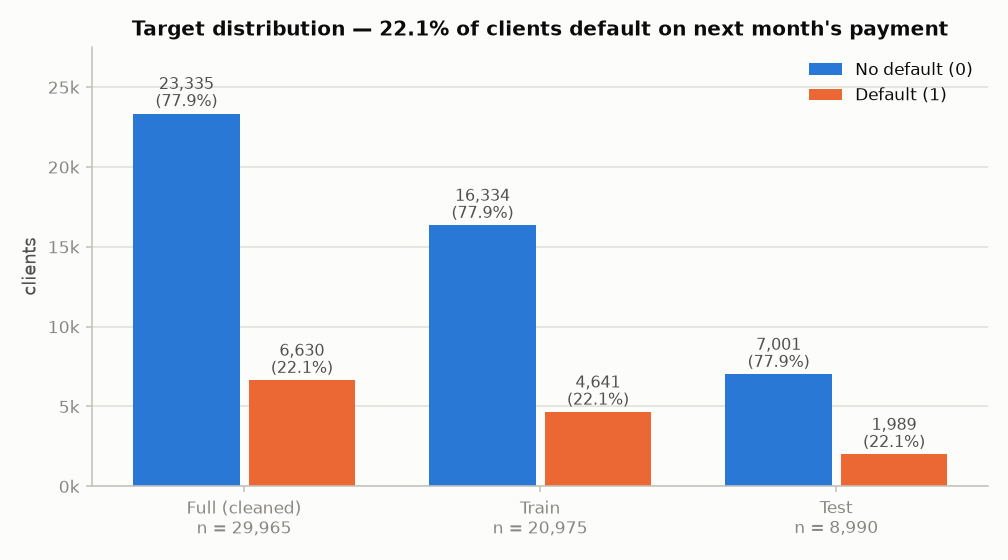
\includegraphics[width=0.92\linewidth]{eda_target_distribution.png}
  \caption{Class balance of the cleaned sample and of the stratified training and test partitions.}
  \label{fig:eda-target-distribution}
\end{figure}

\begin{figure}[htbp]
  \centering
  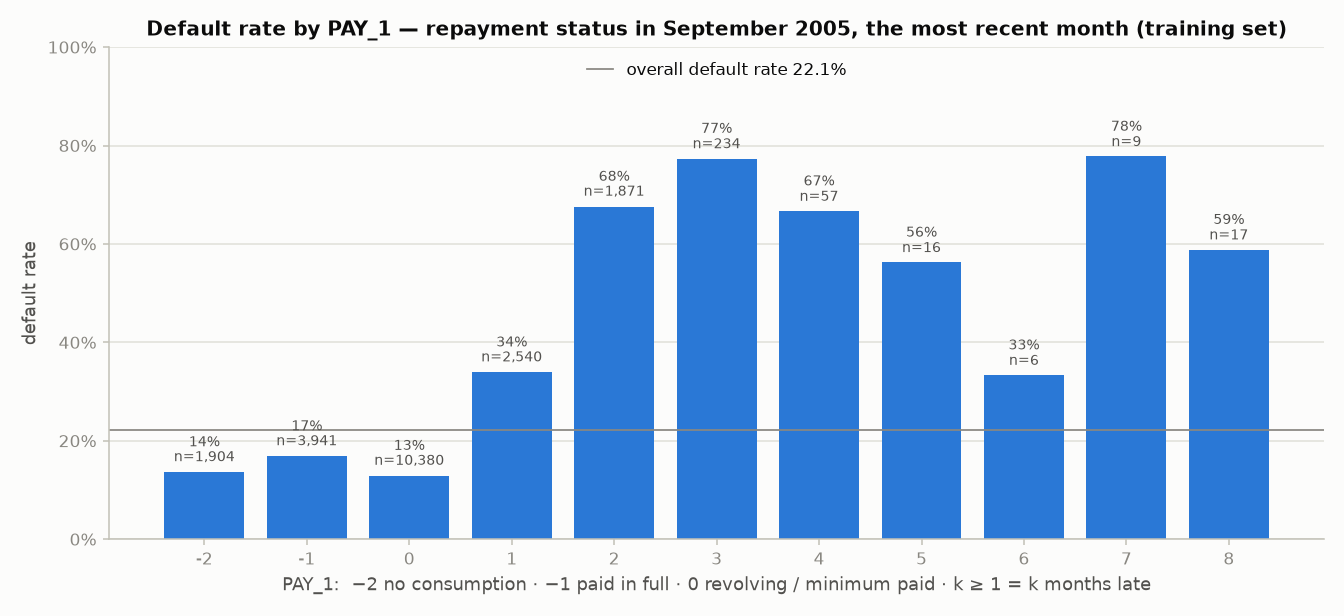
\includegraphics[width=0.92\linewidth]{eda_default_rate_by_pay1.png}
  \caption{Default rate by the most recent repayment status, training partition.}
  \label{fig:eda-default-rate-by-pay1}
\end{figure}

\begin{figure}[htbp]
  \centering
  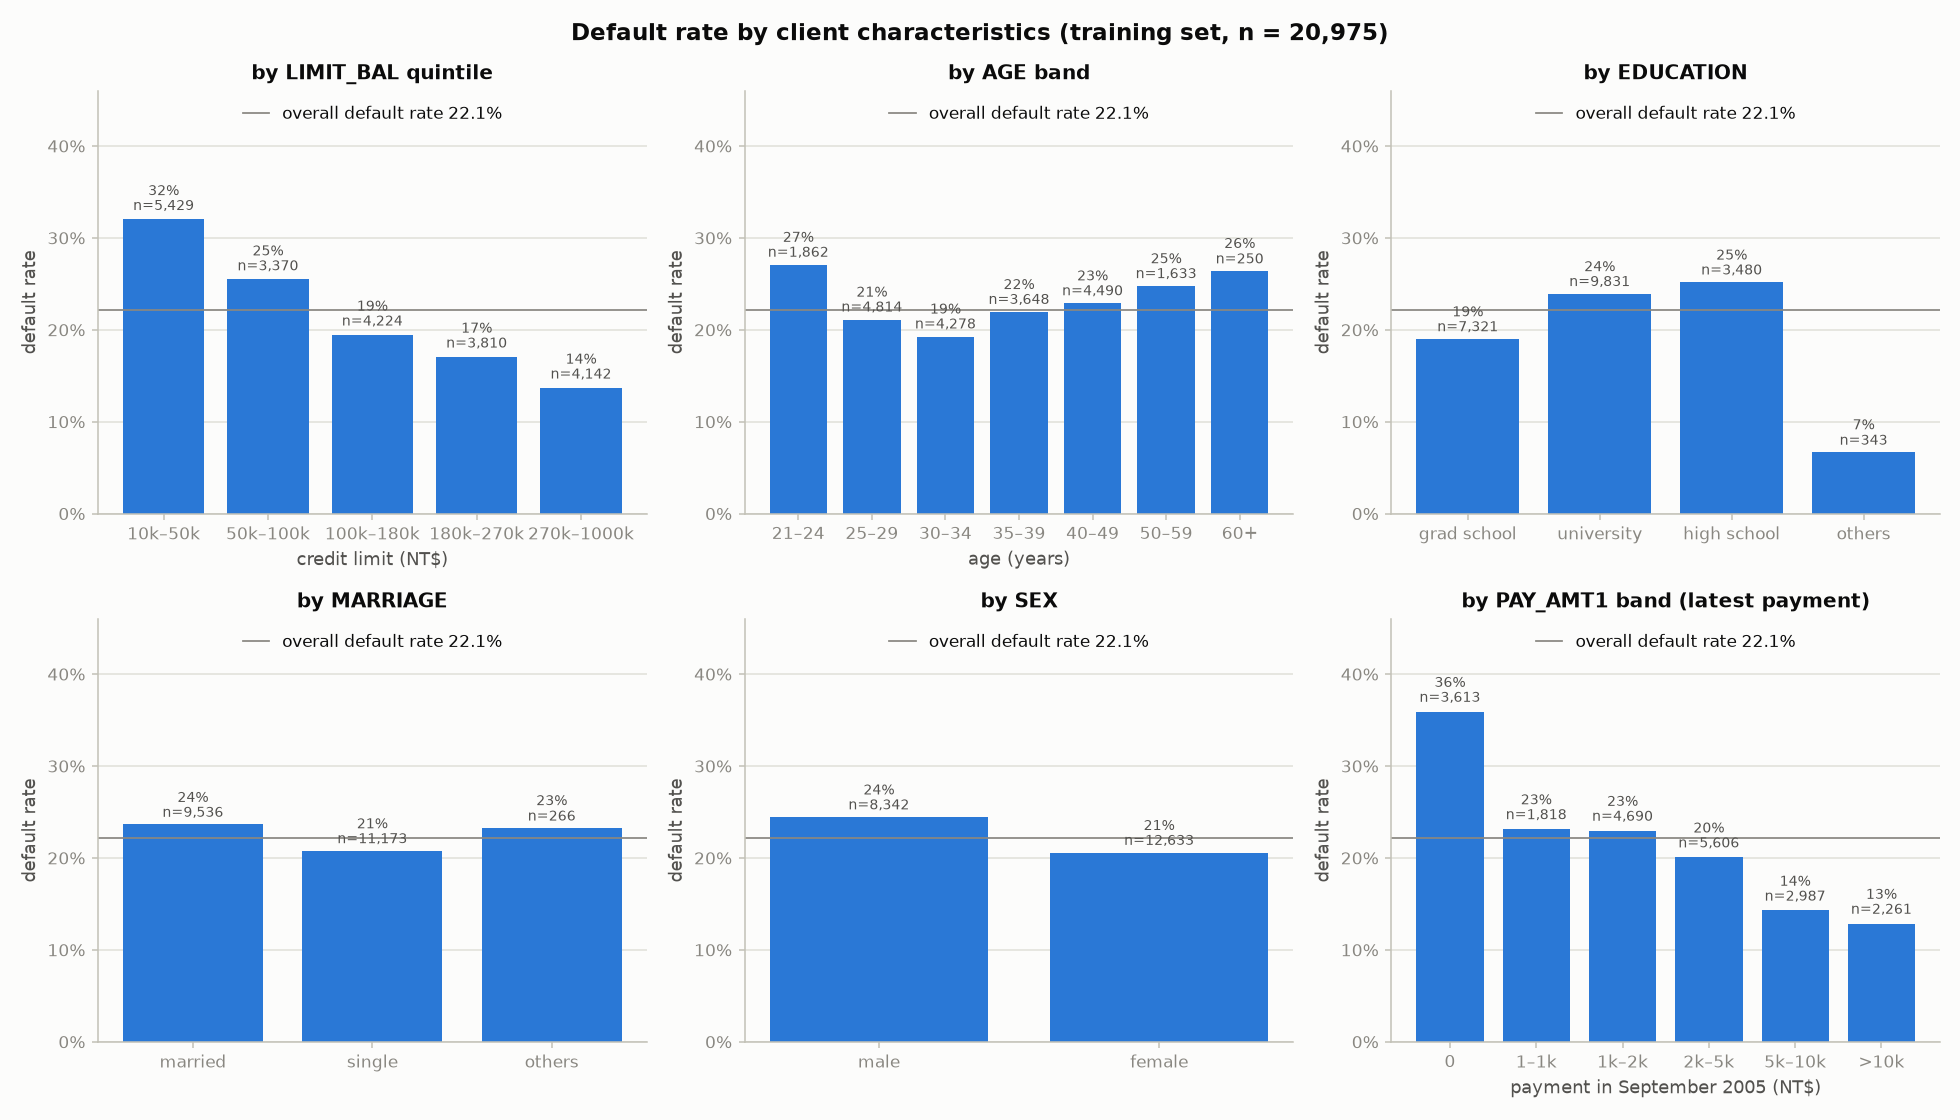
\includegraphics[width=0.92\linewidth]{eda_default_rate_by_groups.png}
  \caption{Training-partition default rate by credit-limit quintile, age band, education, marriage and sex.}
  \label{fig:eda-default-rate-by-groups}
\end{figure}

\begin{figure}[htbp]
  \centering
  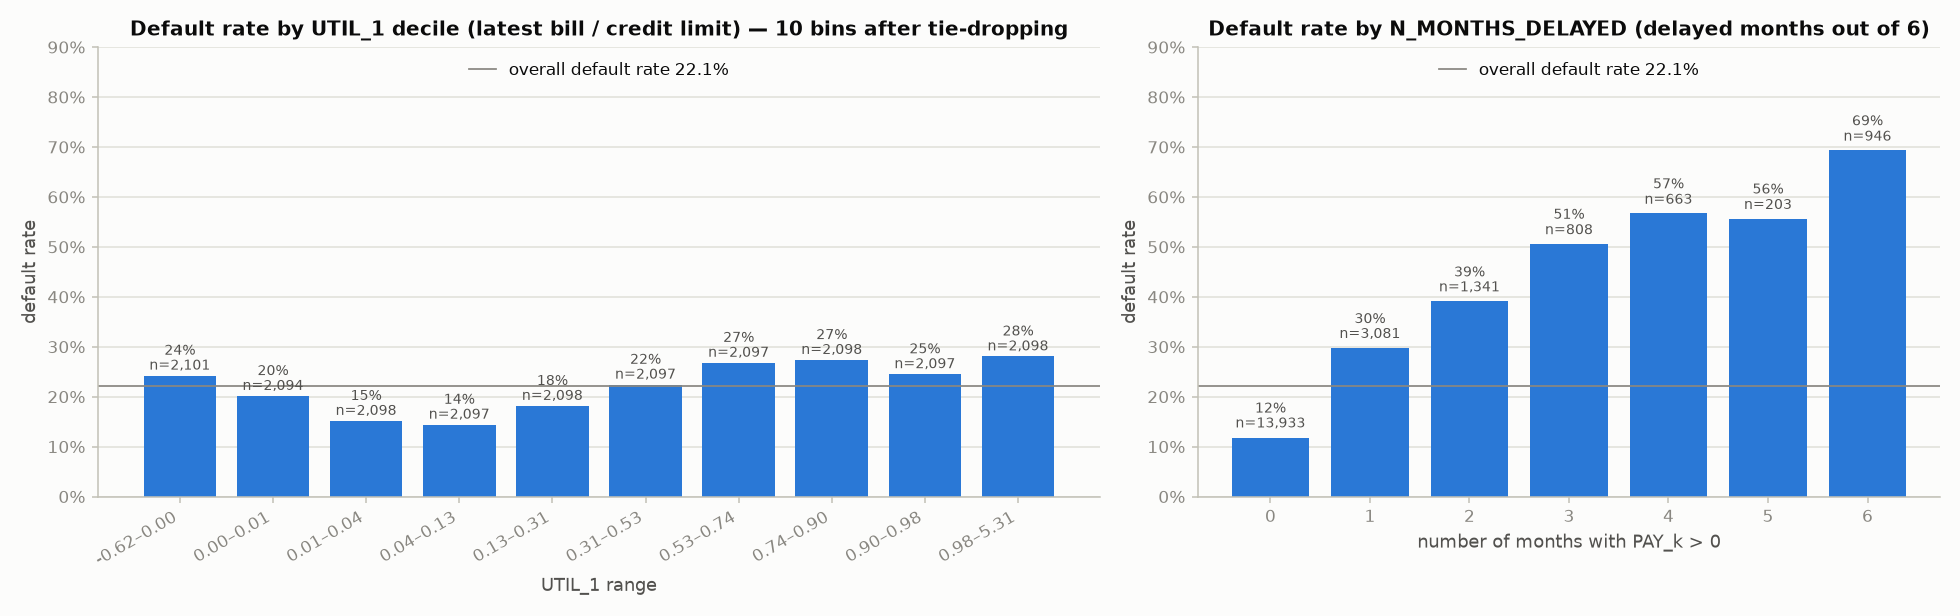
\includegraphics[width=0.92\linewidth]{eda_default_rate_util_delay.png}
  \caption{Default rate by utilisation decile and by number of months in arrears, training partition.}
  \label{fig:eda-default-rate-util-delay}
\end{figure}

\begin{figure}[p]
  \centering
  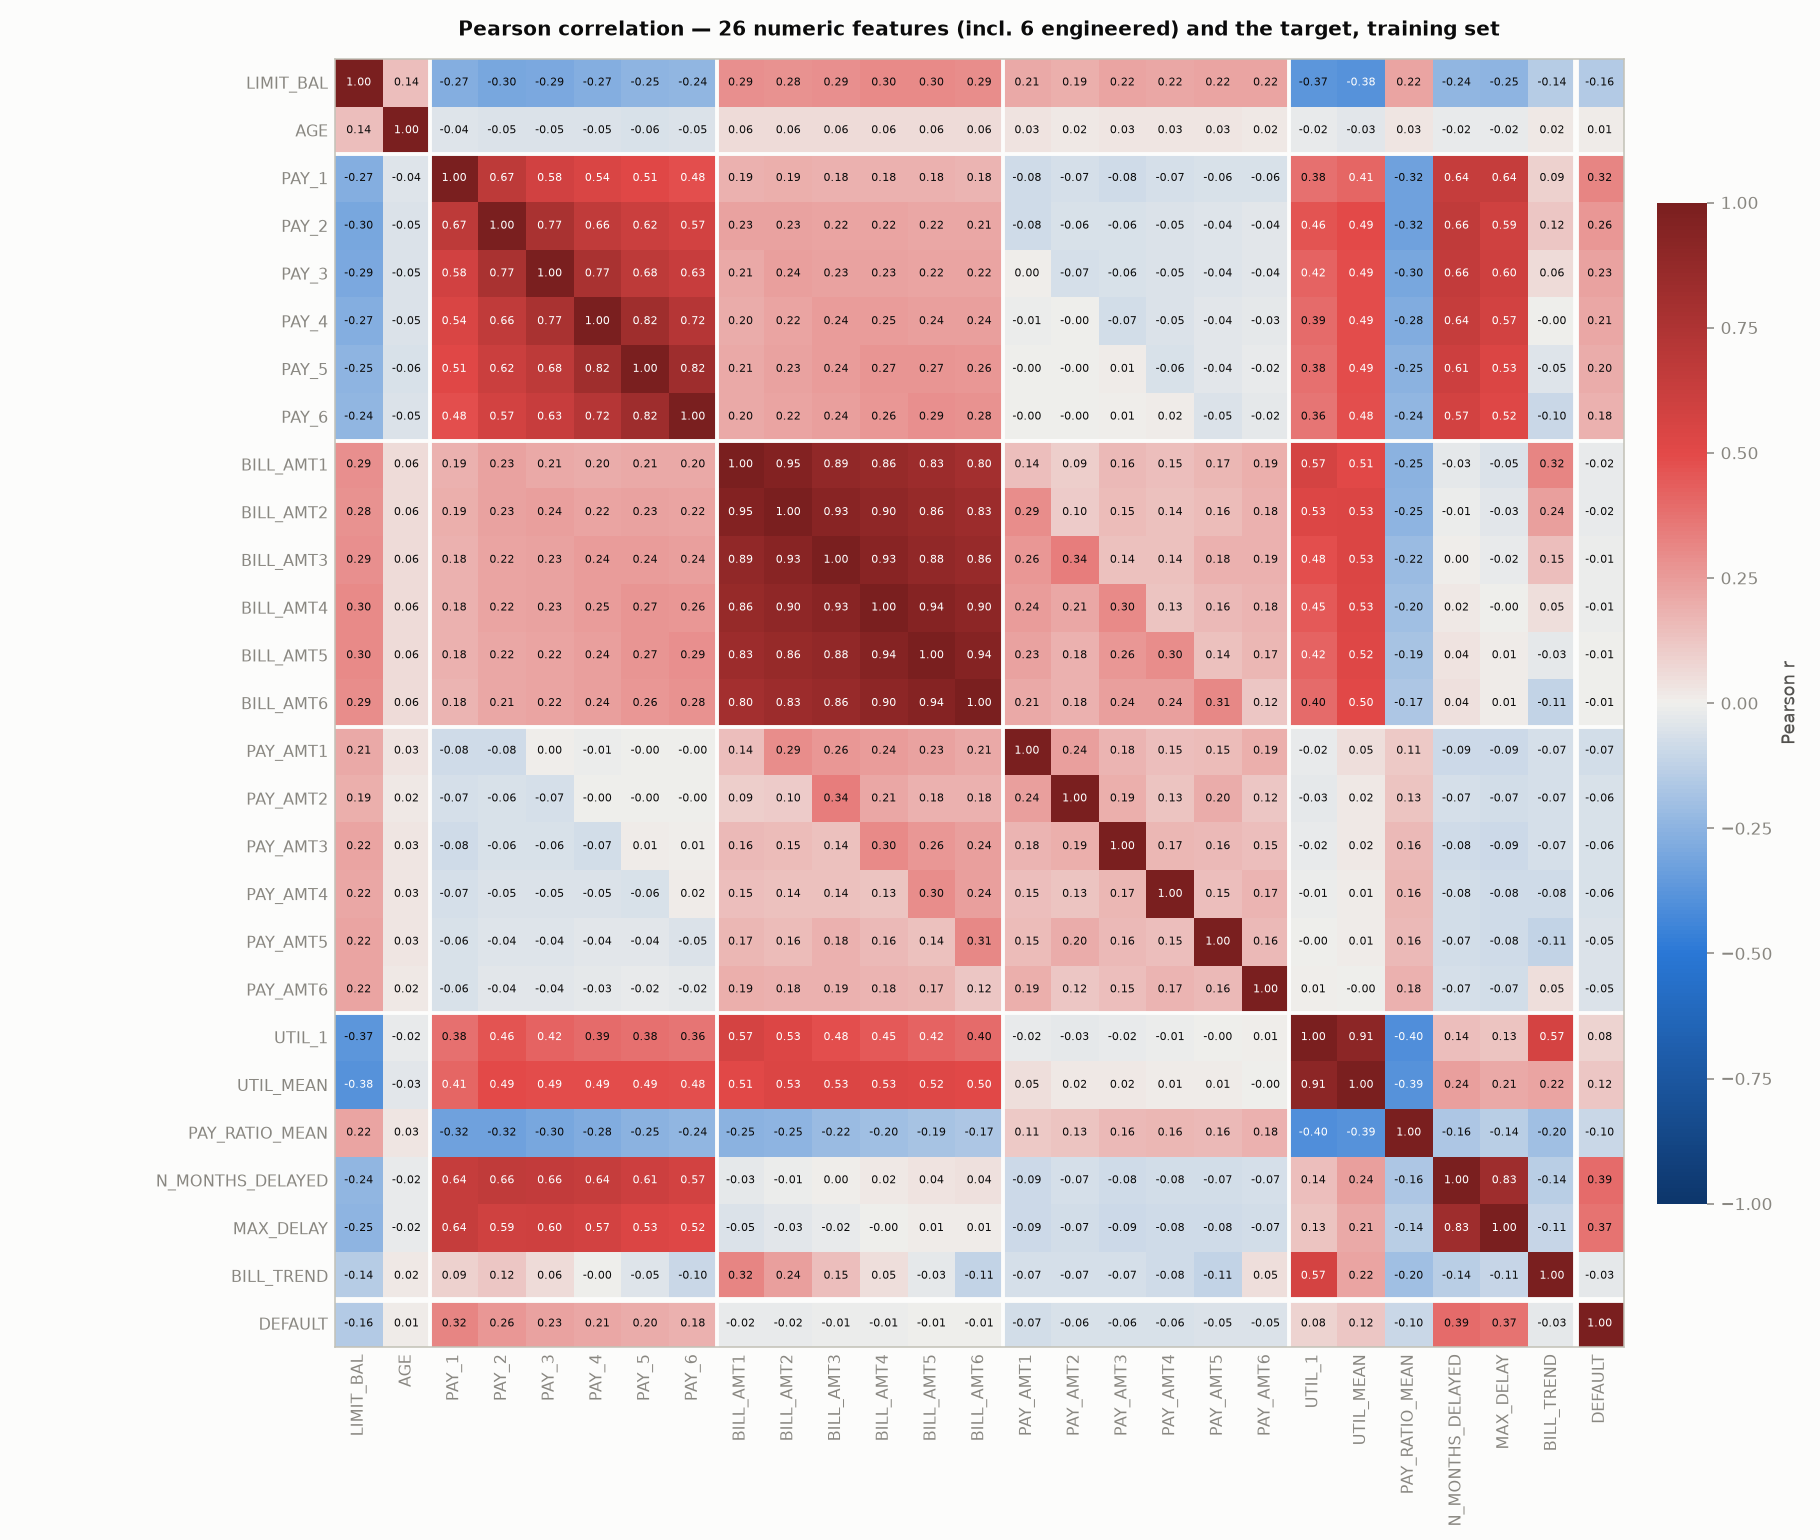
\includegraphics[width=1.0\linewidth]{eda_correlation_heatmap.png}
  \caption{Correlation heat-map of the 29 predictors and the target.}
  \label{fig:eda-correlation-heatmap}
\end{figure}

\begin{figure}[htbp]
  \centering
  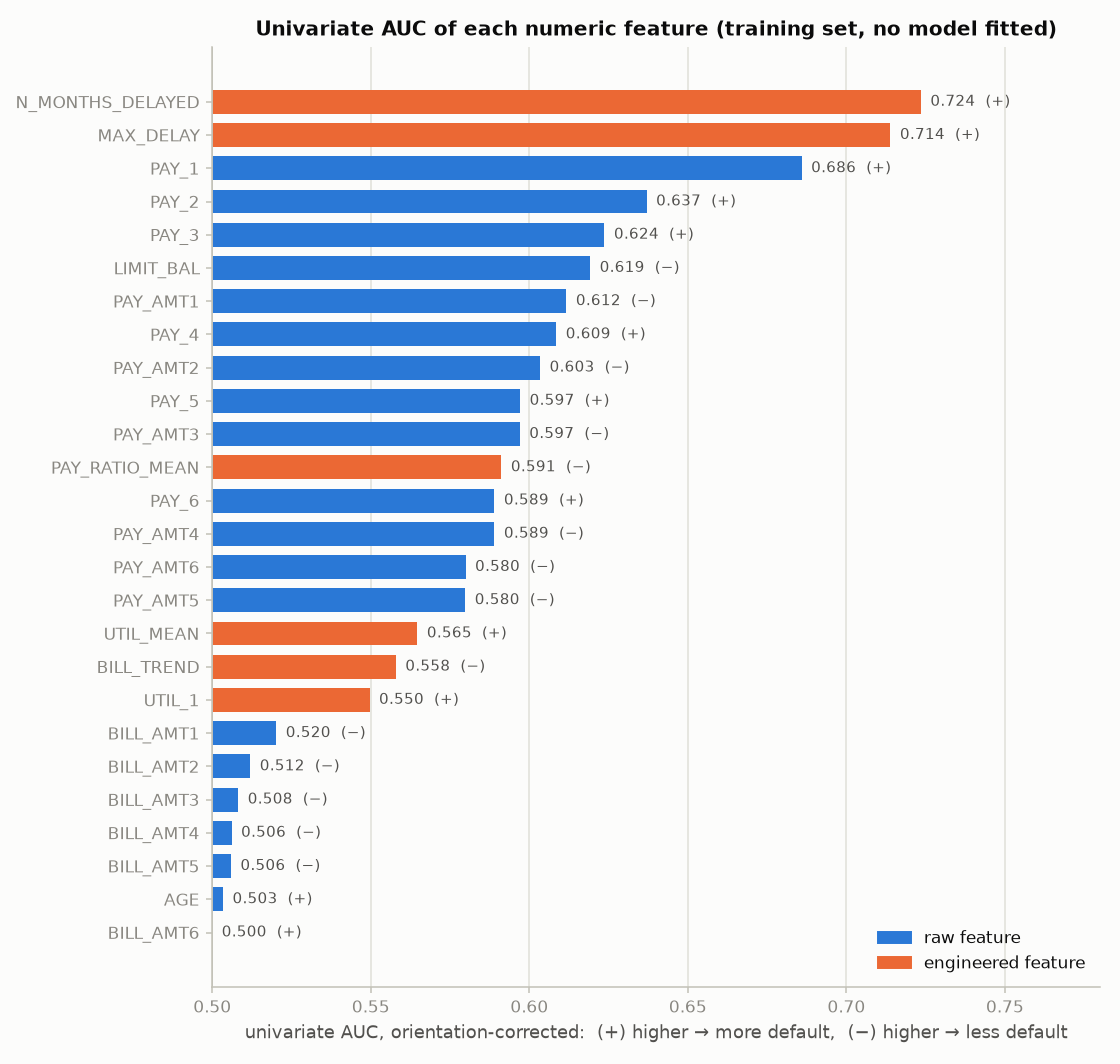
\includegraphics[width=0.92\linewidth]{eda_univariate_strength.png}
  \caption{Univariate strength of every predictor, as an oriented AUC.}
  \label{fig:eda-univariate-strength}
\end{figure}
\clearpage

\begin{figure}[htbp]
  \centering
  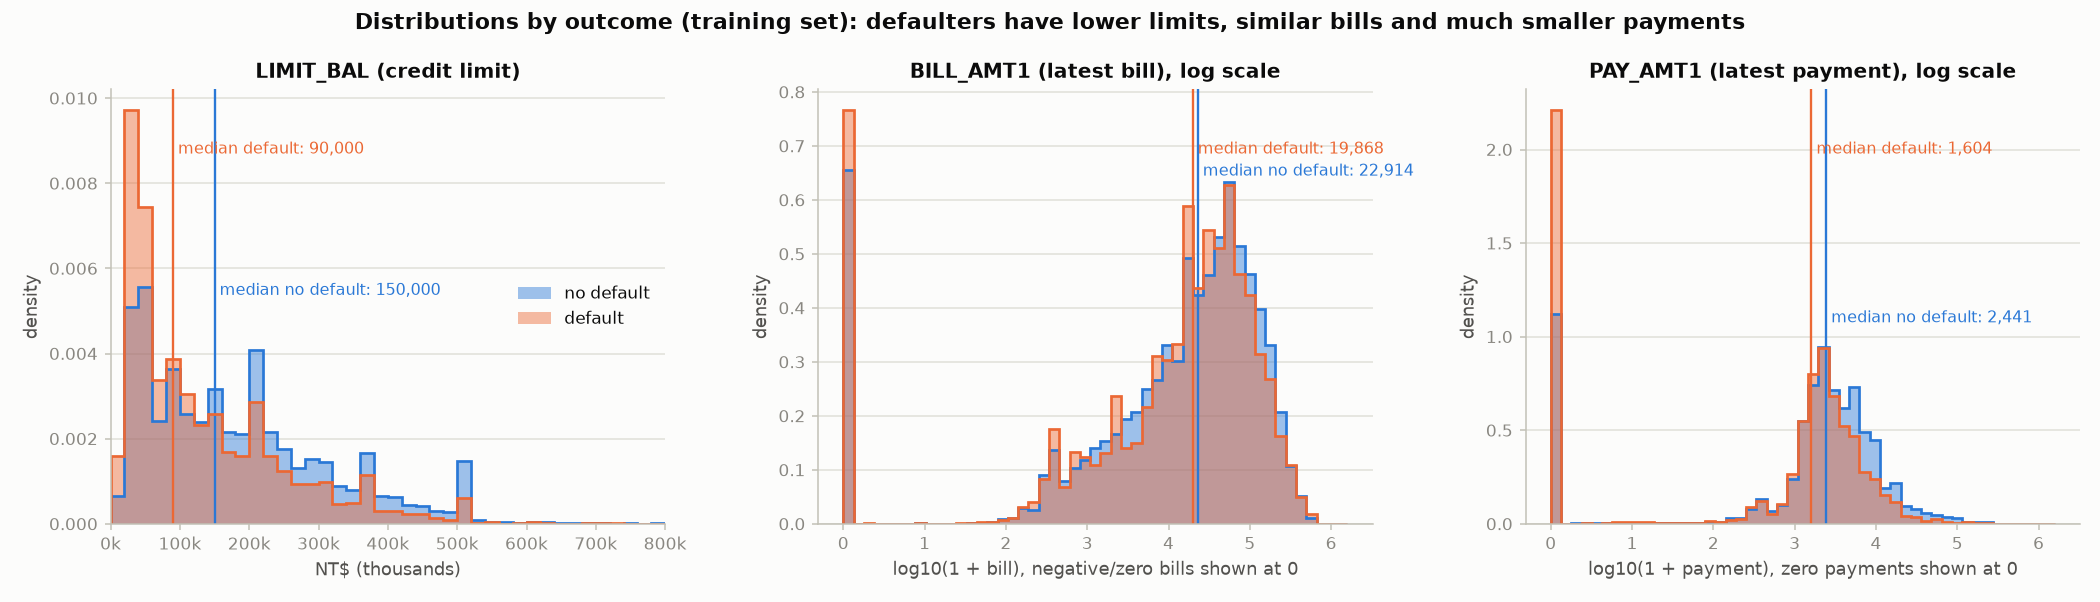
\includegraphics[width=0.92\linewidth]{eda_distributions_by_default.png}
  \caption{Distributions of the main numeric features by class, training partition.}
  \label{fig:eda-distributions-by-default}
\end{figure}

\clearpage
\subsection{Model comparison}

\begin{figure}[htbp]
  \centering
  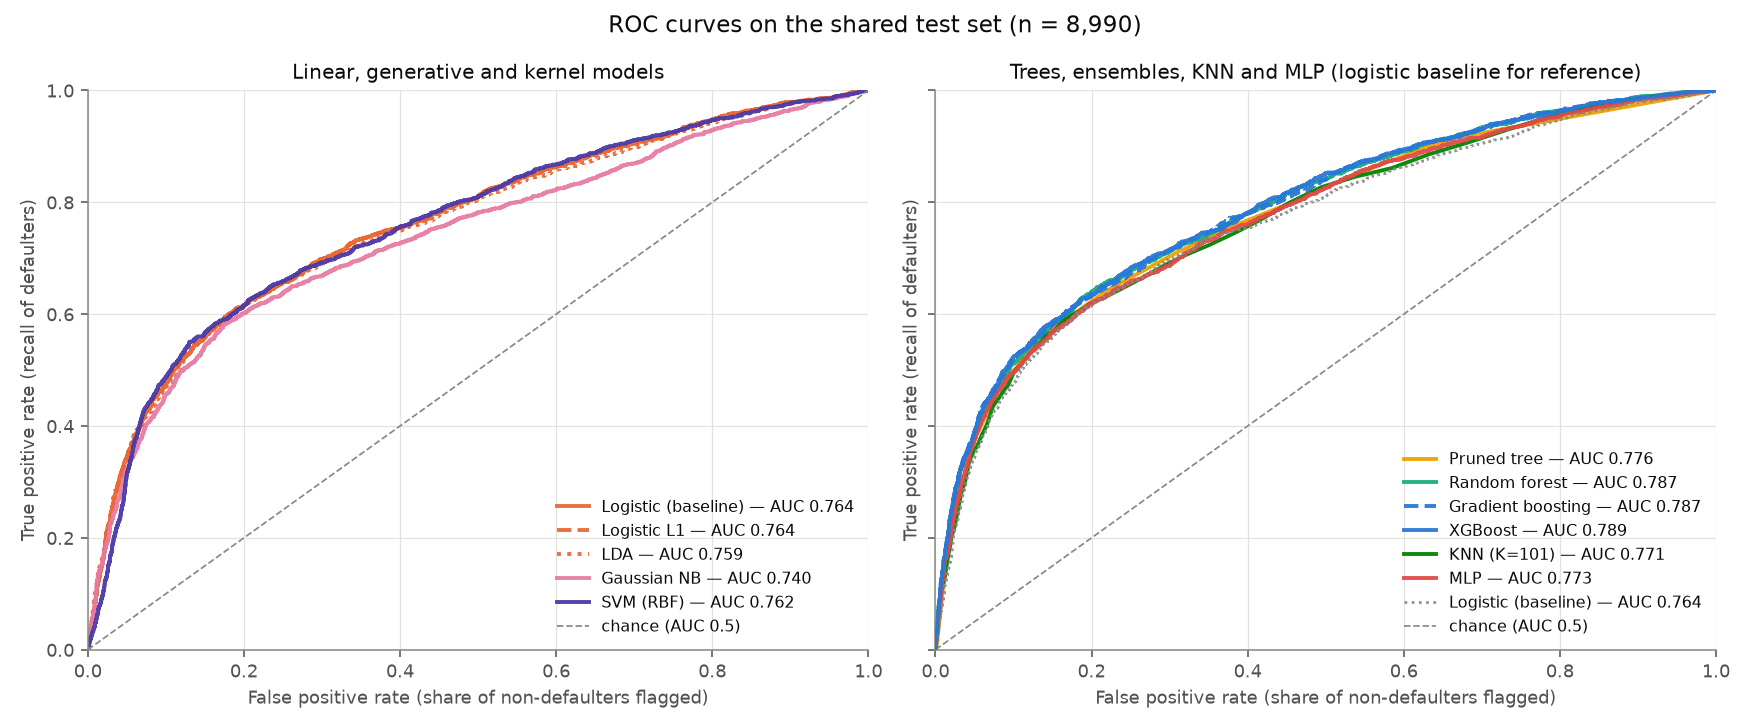
\includegraphics[width=0.92\linewidth]{all_roc.png}
  \caption{Test-set ROC curves of the headline models.}
  \label{fig:all-roc}
\end{figure}

\begin{figure}[htbp]
  \centering
  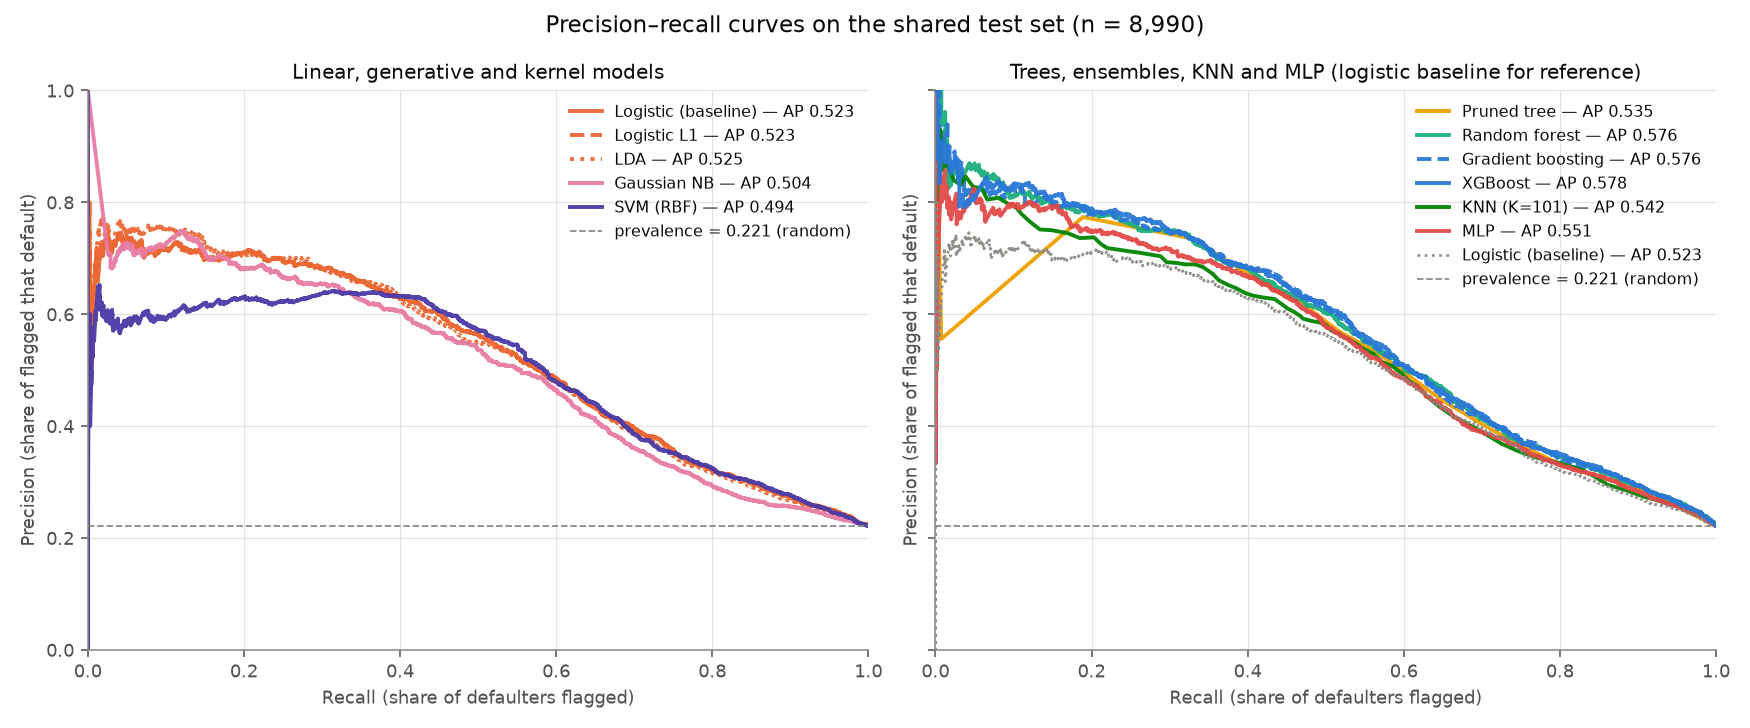
\includegraphics[width=0.92\linewidth]{all_pr.png}
  \caption{Test-set precision--recall curves; the horizontal line is the prevalence.}
  \label{fig:all-pr}
\end{figure}

\begin{figure}[htbp]
  \centering
  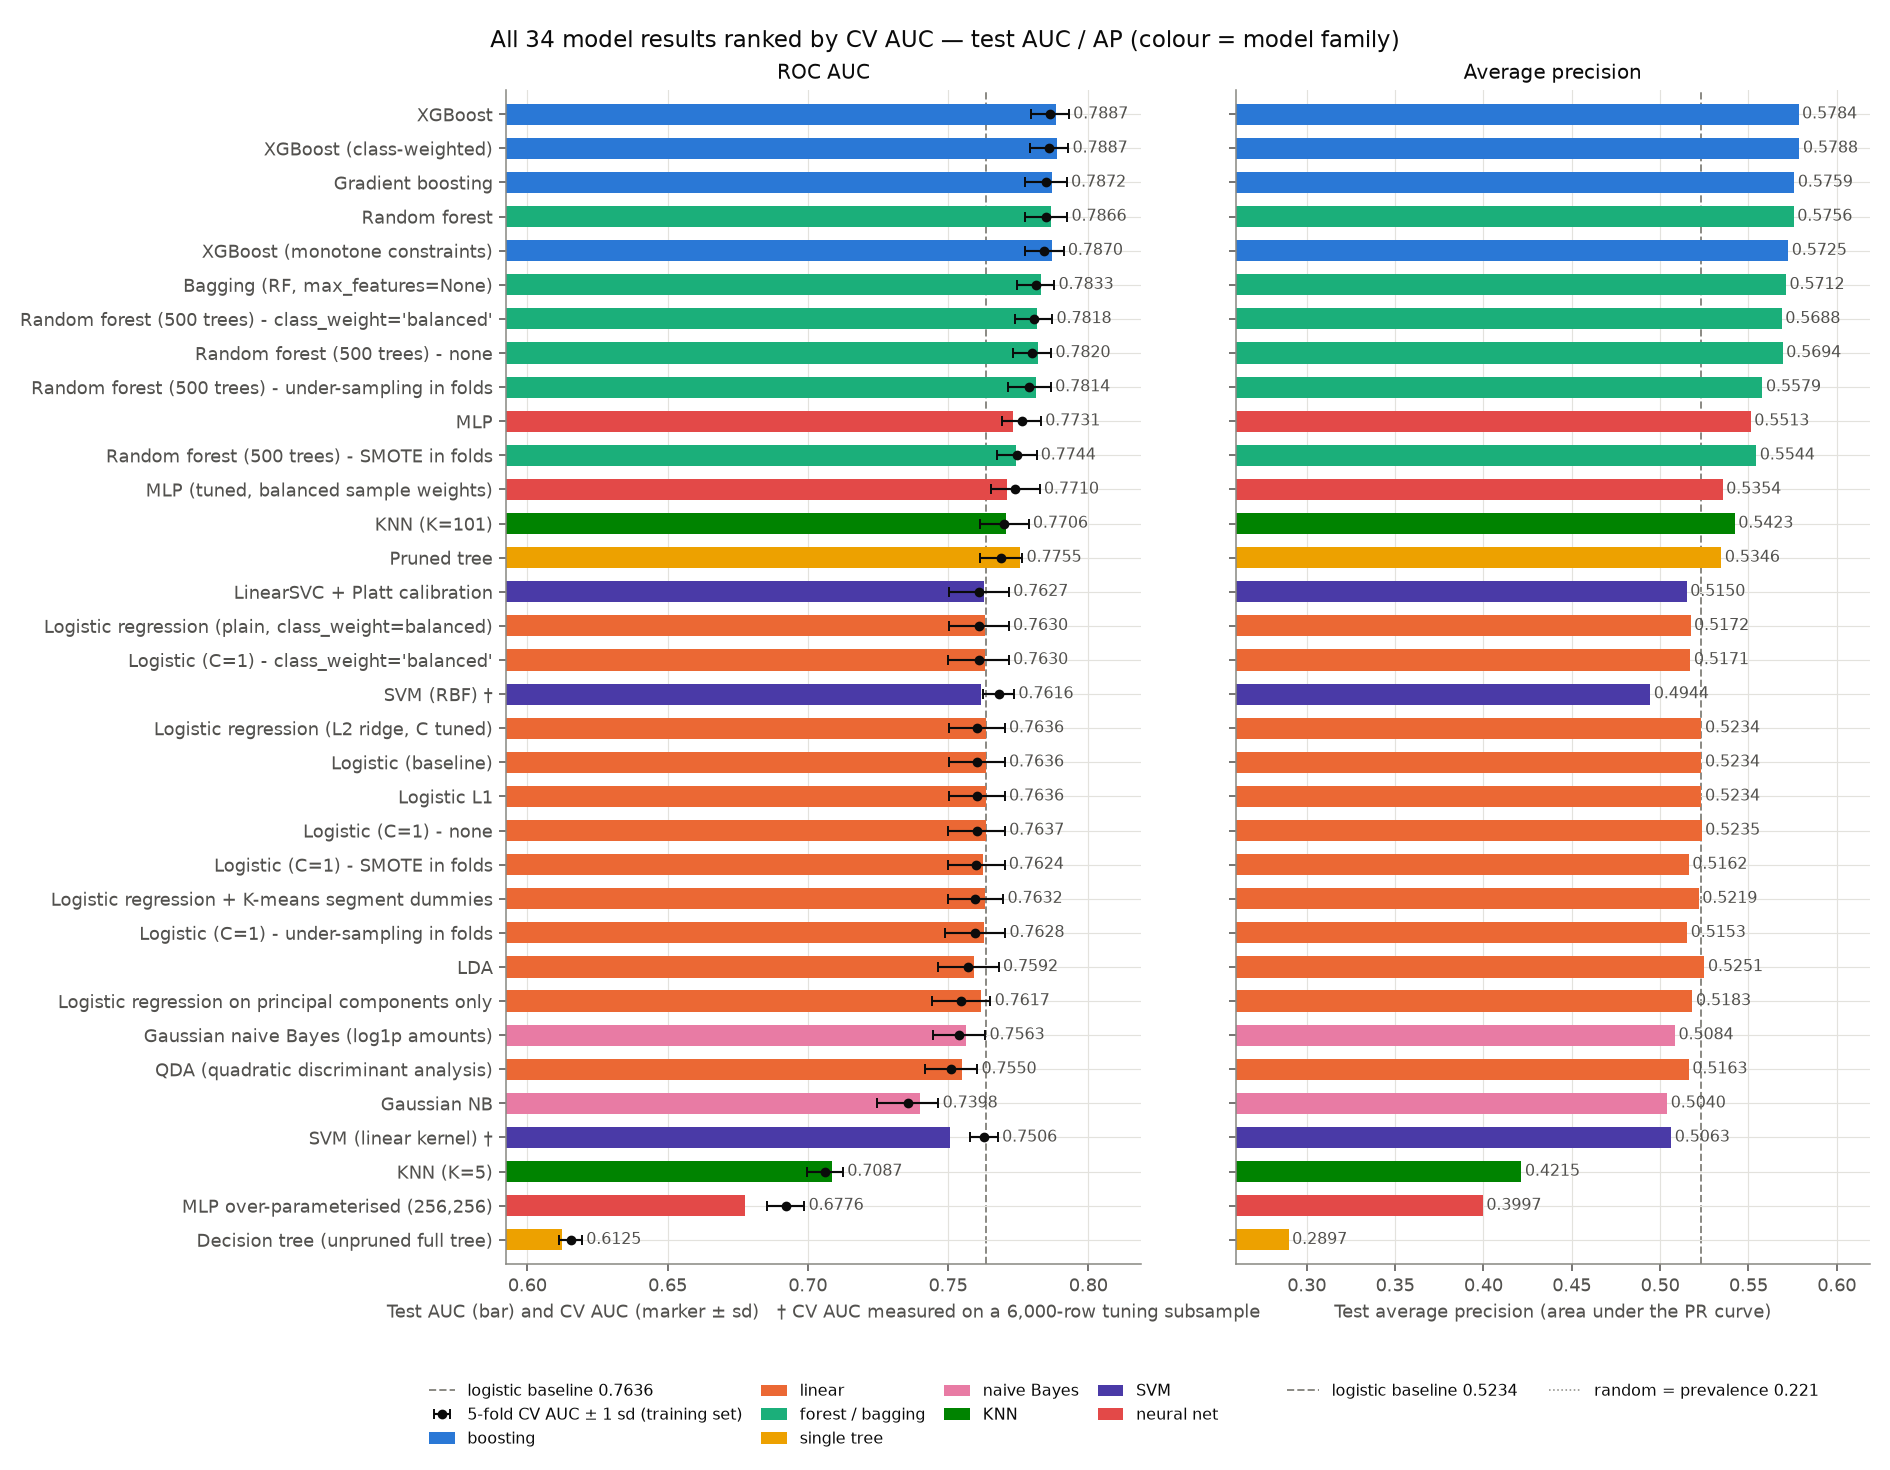
\includegraphics[width=0.92\linewidth]{all_auc_bar_full.png}
  \caption{Test AUC of every model variant fitted, ordered by CV AUC, with the benchmark marked.}
  \label{fig:all-auc-bar-full}
\end{figure}

\begin{figure}[htbp]
  \centering
  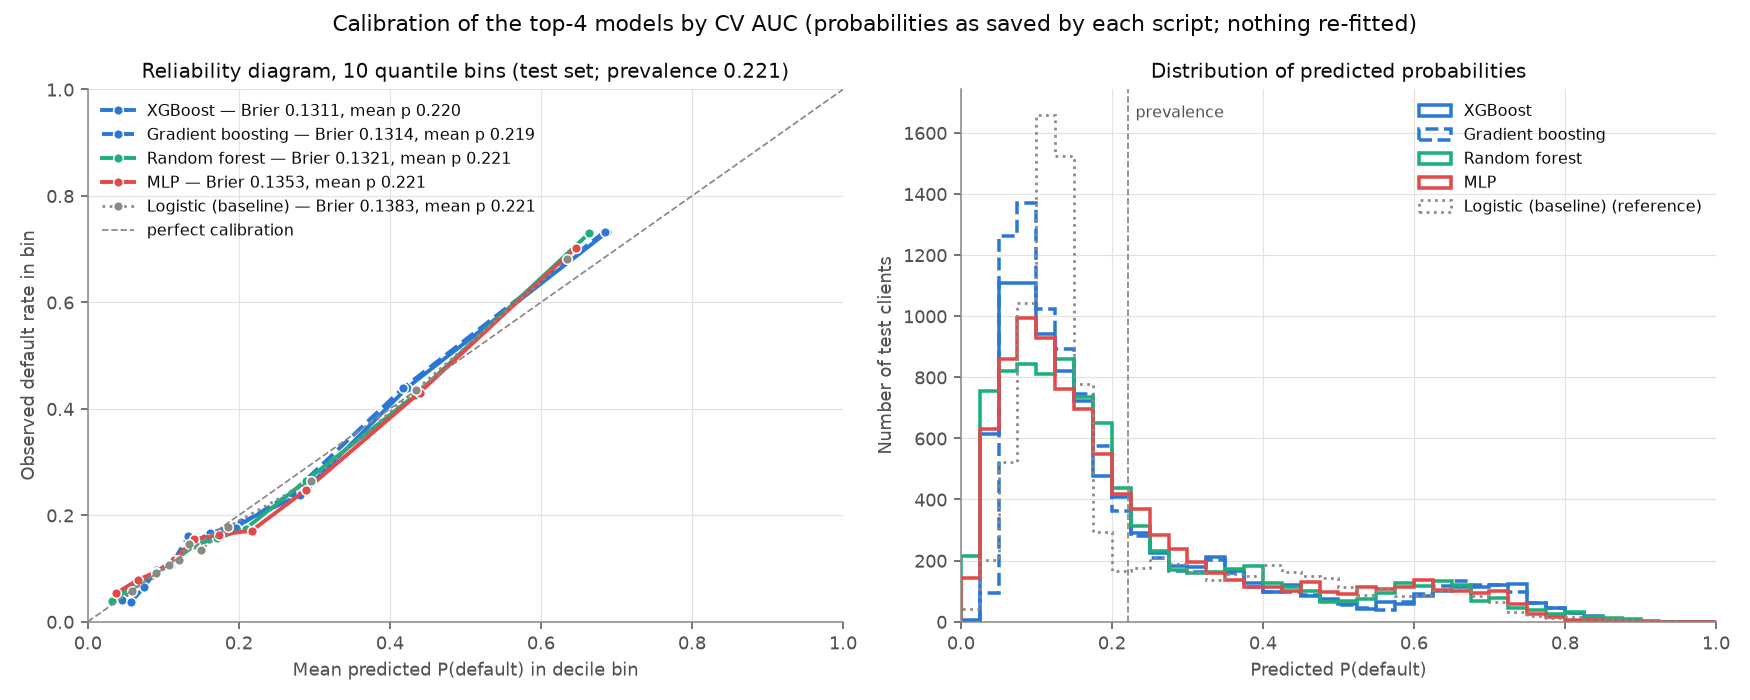
\includegraphics[width=0.92\linewidth]{calibration.png}
  \caption{Calibration curves of the four models with the highest CV AUC: predicted against observed default rate by decile of score.}
  \label{fig:calibration}
\end{figure}

\begin{figure}[htbp]
  \centering
  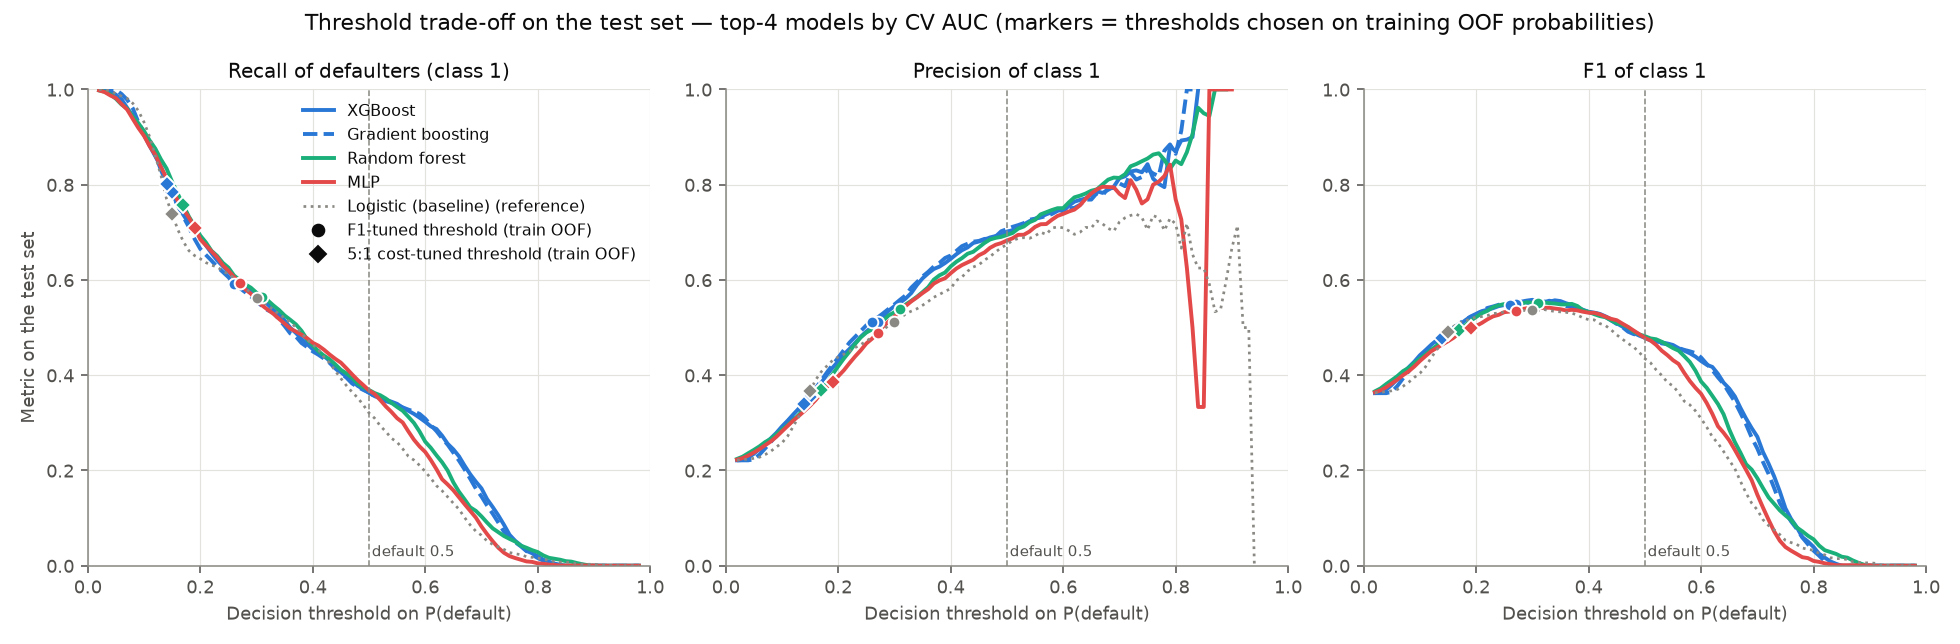
\includegraphics[width=0.92\linewidth]{threshold_curves.png}
  \caption{Recall, precision and F1 against the decision threshold.}
  \label{fig:threshold-curves}
\end{figure}
\clearpage

\begin{figure}[htbp]
  \centering
  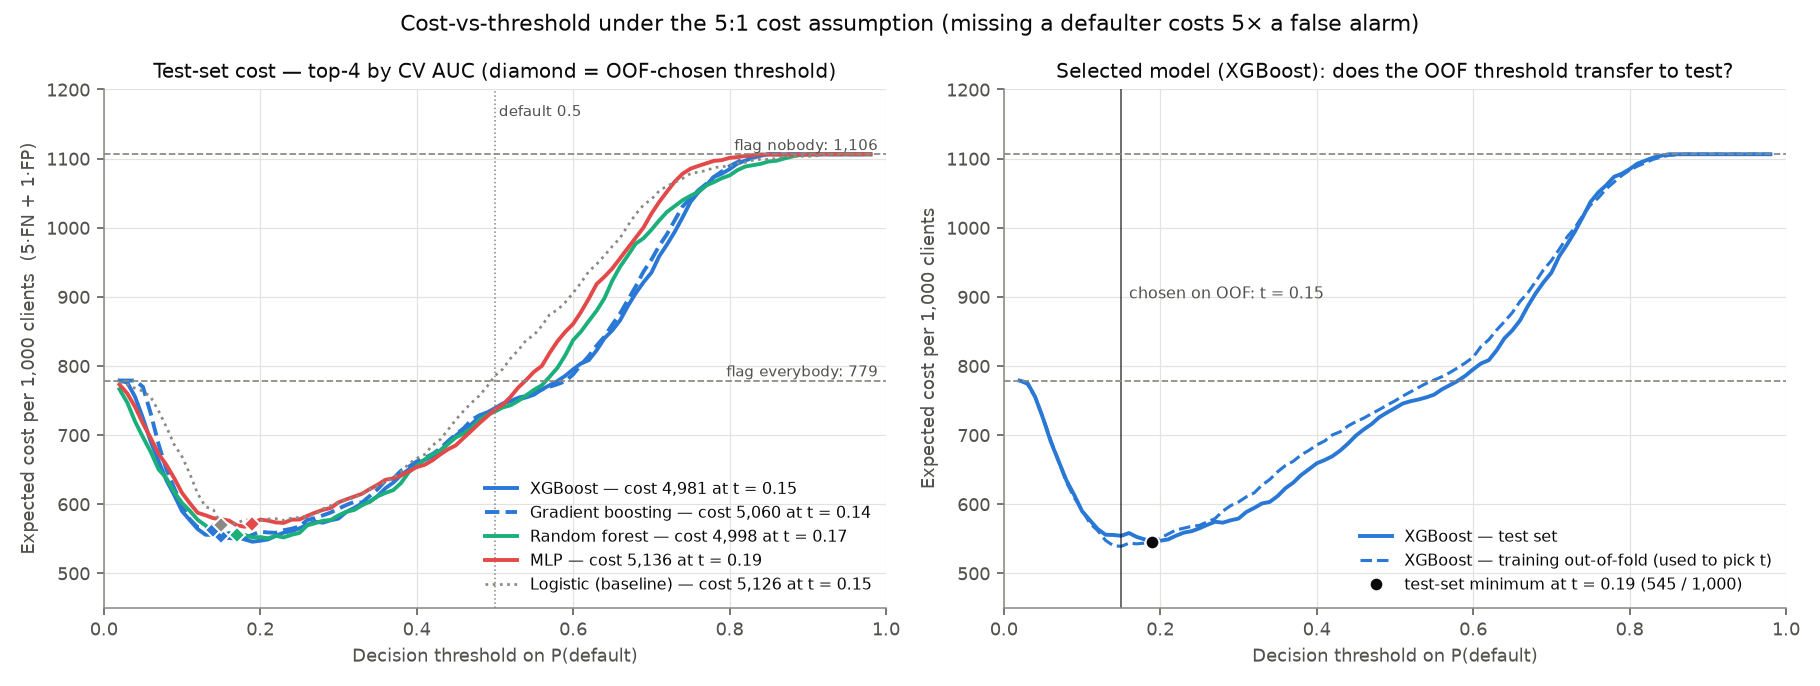
\includegraphics[width=0.92\linewidth]{cost_curves.png}
  \caption{Expected cost against the decision threshold at a 5:1 ratio.}
  \label{fig:cost-curves}
\end{figure}

\begin{figure}[htbp]
  \centering
  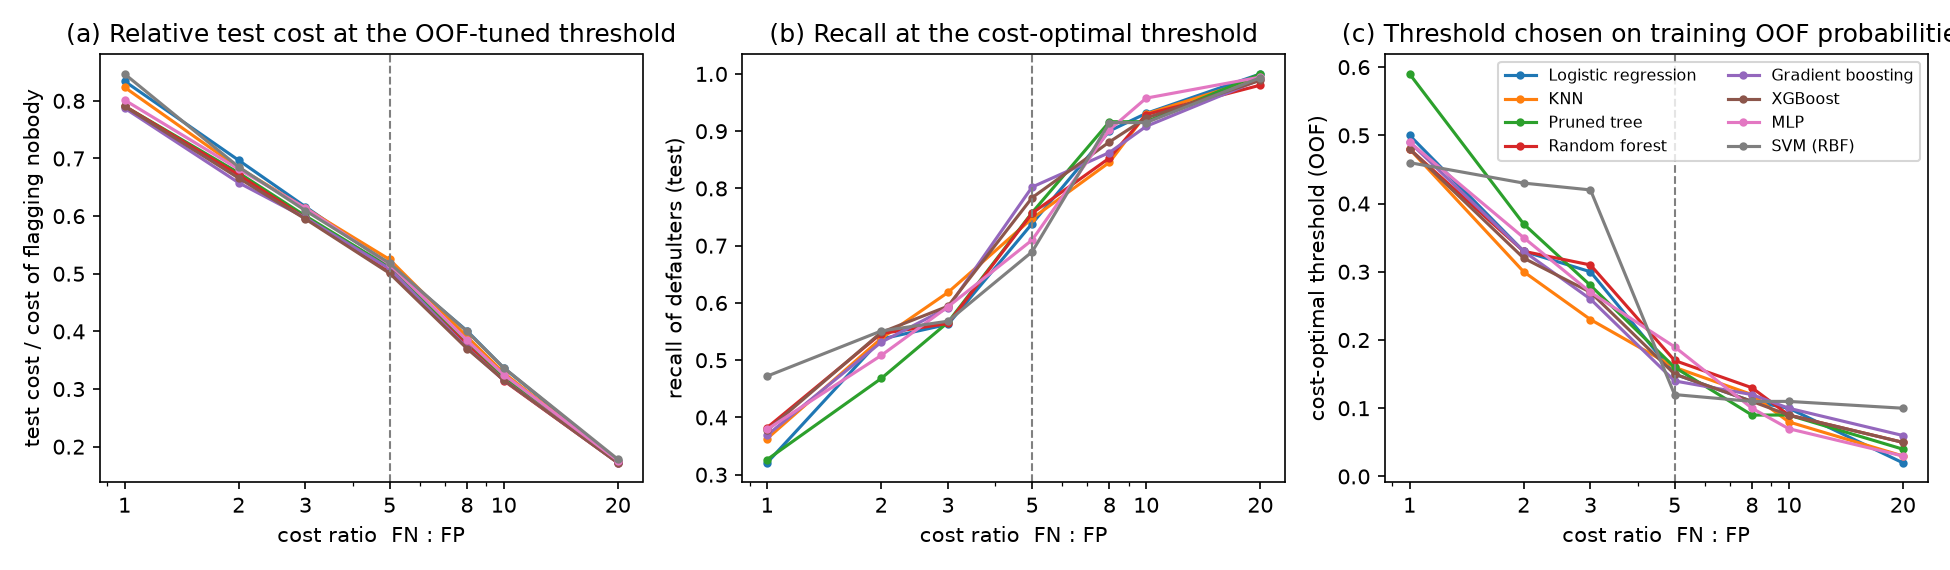
\includegraphics[width=0.92\linewidth]{cost_sensitivity.png}
  \caption{Cost-minimising threshold and cost as the cost ratio varies from 1:1 to 20:1.}
  \label{fig:cost-sensitivity}
\end{figure}

\begin{figure}[htbp]
  \centering
  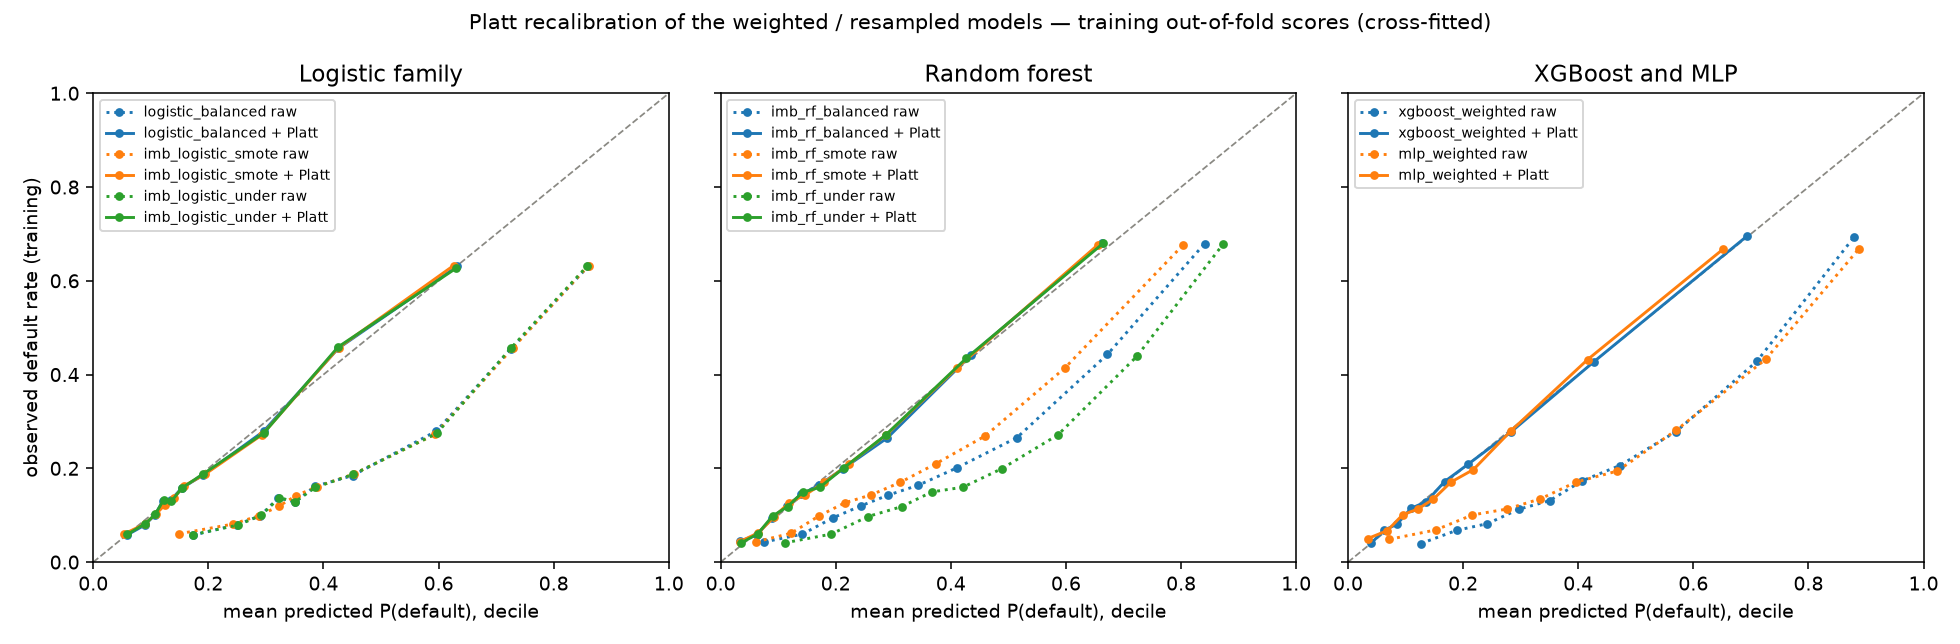
\includegraphics[width=0.92\linewidth]{recalibration.png}
  \caption{Reliability of the nine weighted or resampled models before and after Platt recalibration, on training out-of-fold scores.}
  \label{fig:recalibration}
\end{figure}

\clearpage
\subsection{Interpretation}

\begin{figure}[htbp]
  \centering
  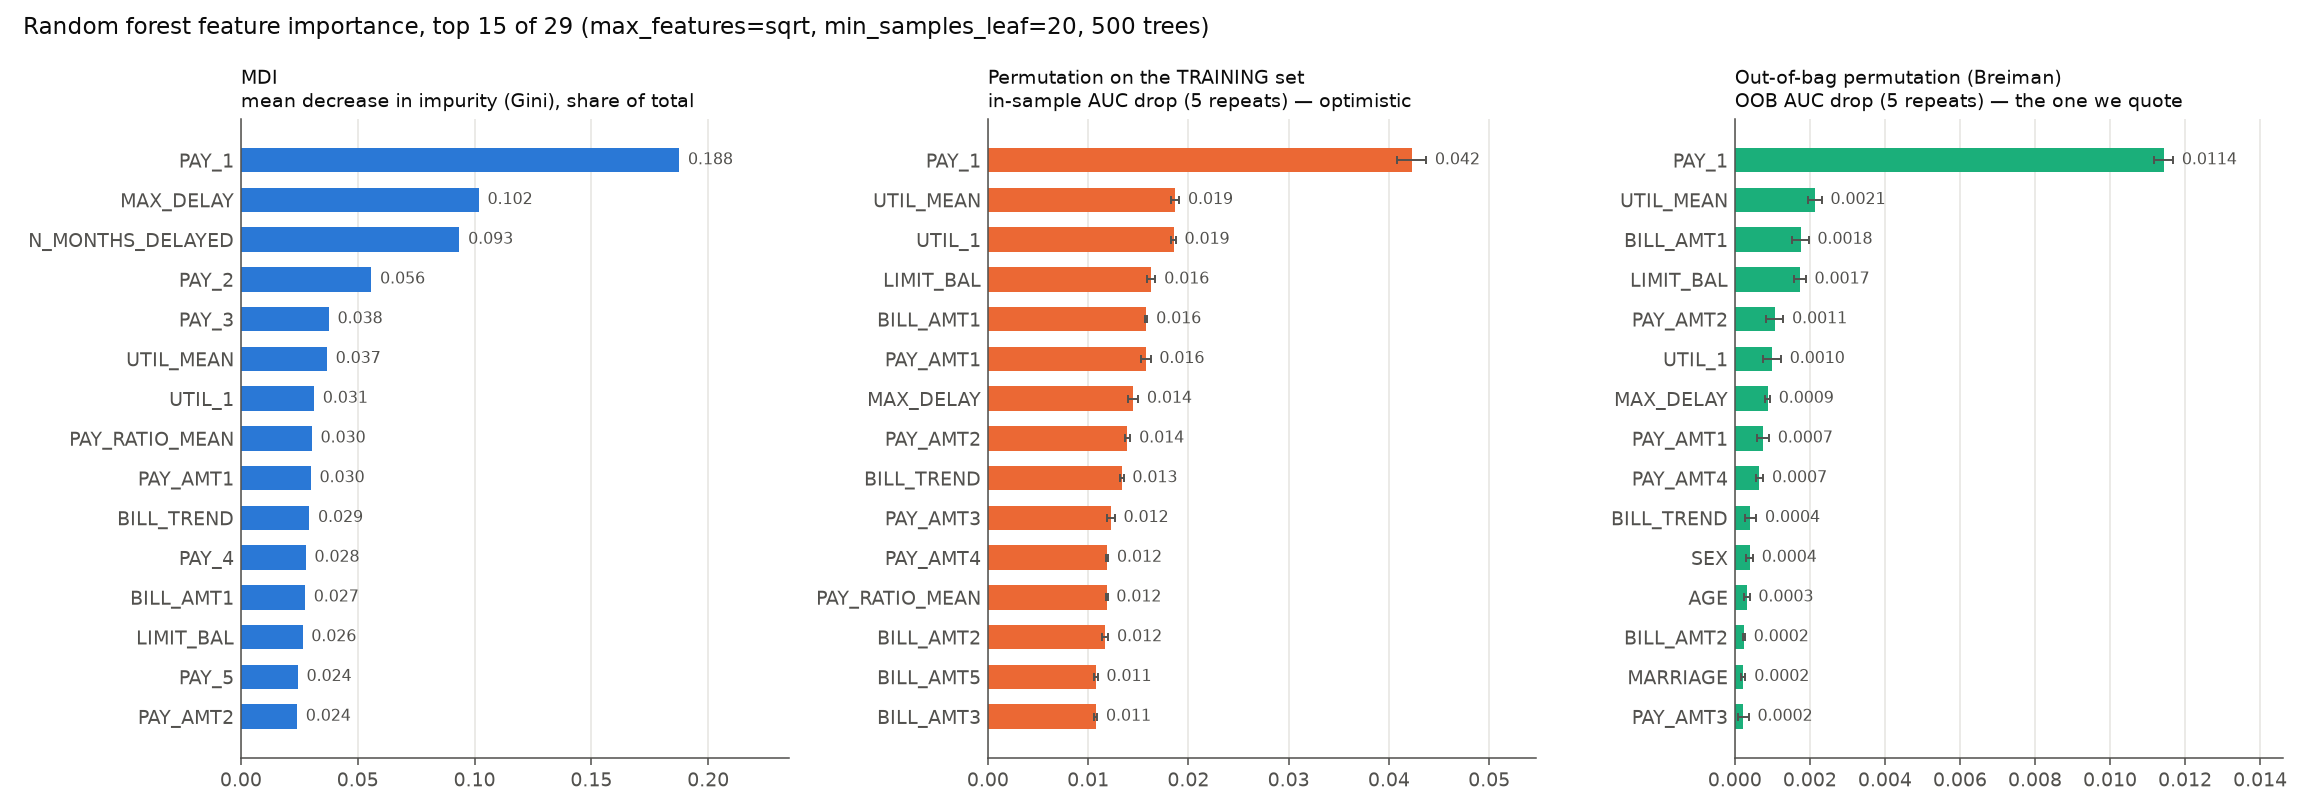
\includegraphics[width=0.92\linewidth]{rf_importance.png}
  \caption{Random forest importances: impurity decrease, training-set permutation and out-of-bag permutation, side by side.}
  \label{fig:rf-importance}
\end{figure}

\begin{figure}[htbp]
  \centering
  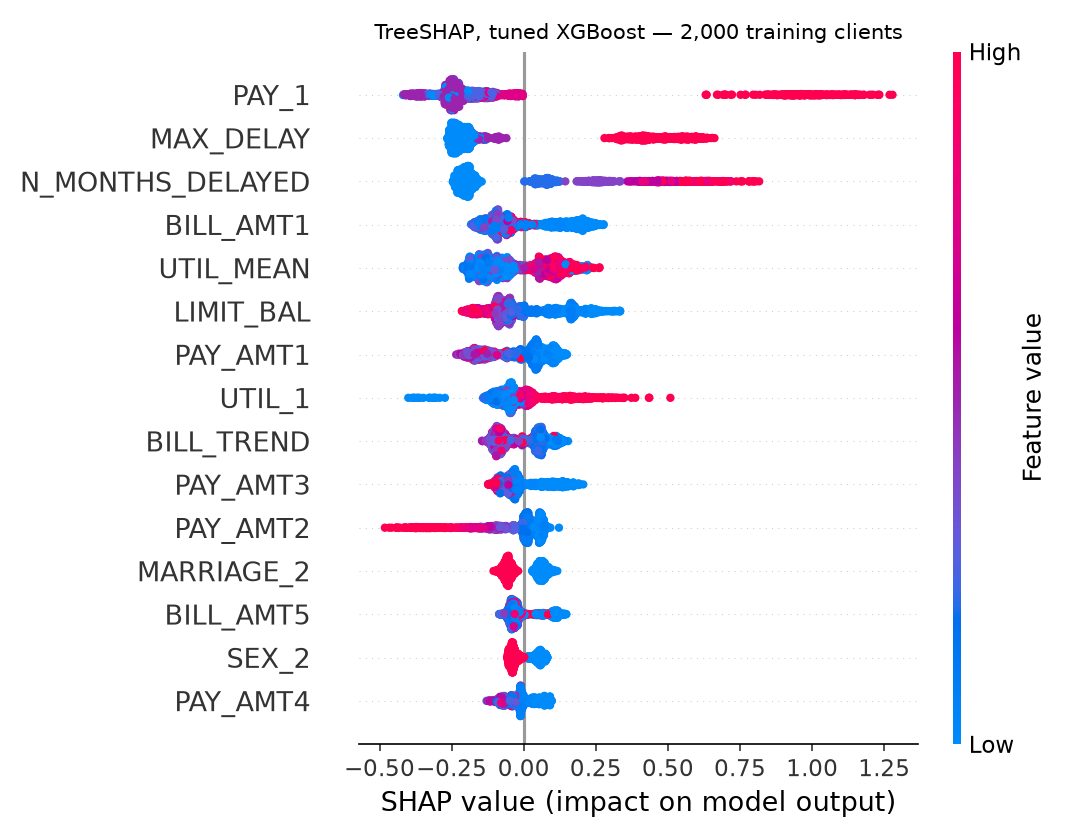
\includegraphics[width=0.92\linewidth]{shap_beeswarm.png}
  \caption{TreeSHAP beeswarm for the tuned XGBoost over training clients.}
  \label{fig:shap-beeswarm}
\end{figure}

\begin{figure}[htbp]
  \centering
  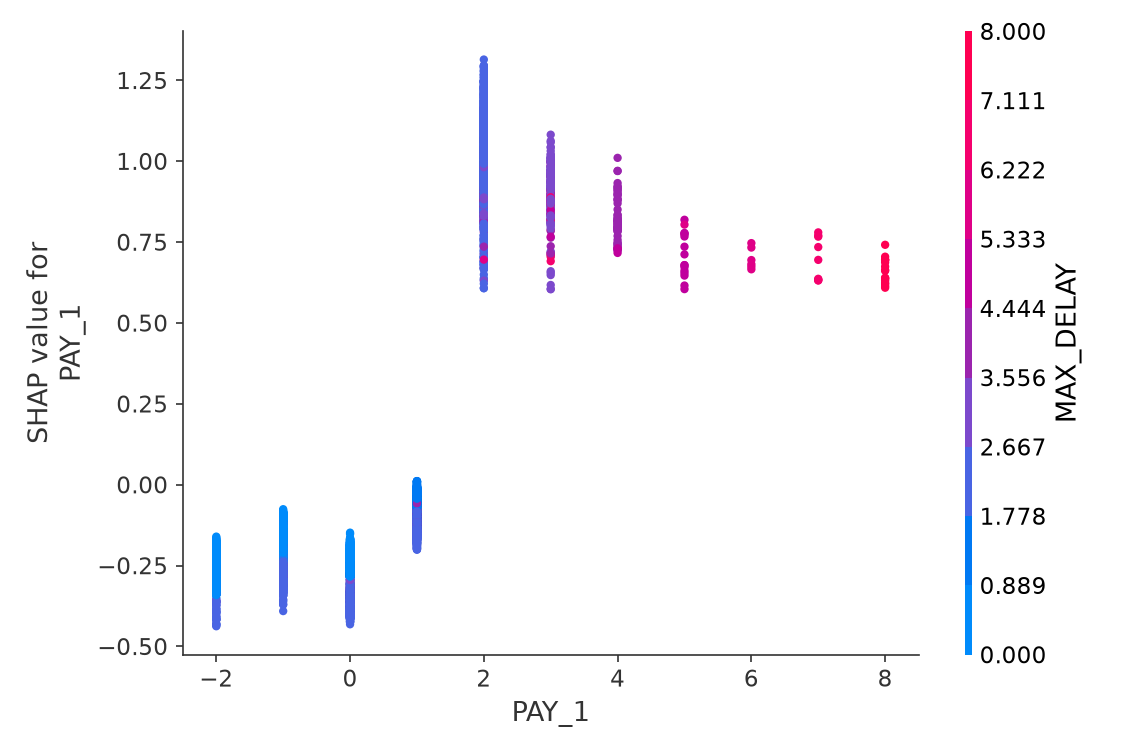
\includegraphics[width=0.92\linewidth]{shap_dependence_pay1.png}
  \caption{TreeSHAP dependence plot for the most recent repayment status.}
  \label{fig:shap-dependence-pay1}
\end{figure}
\clearpage

\begin{figure}[htbp]
  \centering
  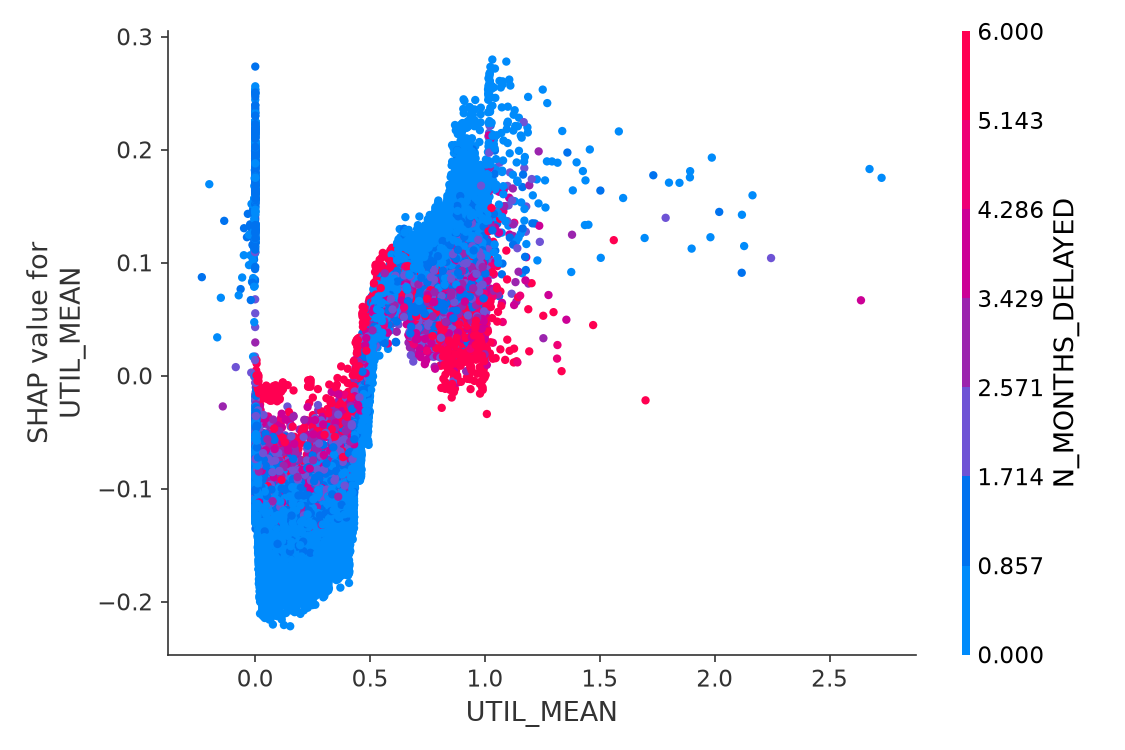
\includegraphics[width=0.92\linewidth]{shap_dependence_util_mean.png}
  \caption{TreeSHAP dependence plot for mean utilisation.}
  \label{fig:shap-dependence-util-mean}
\end{figure}

\begin{figure}[htbp]
  \centering
  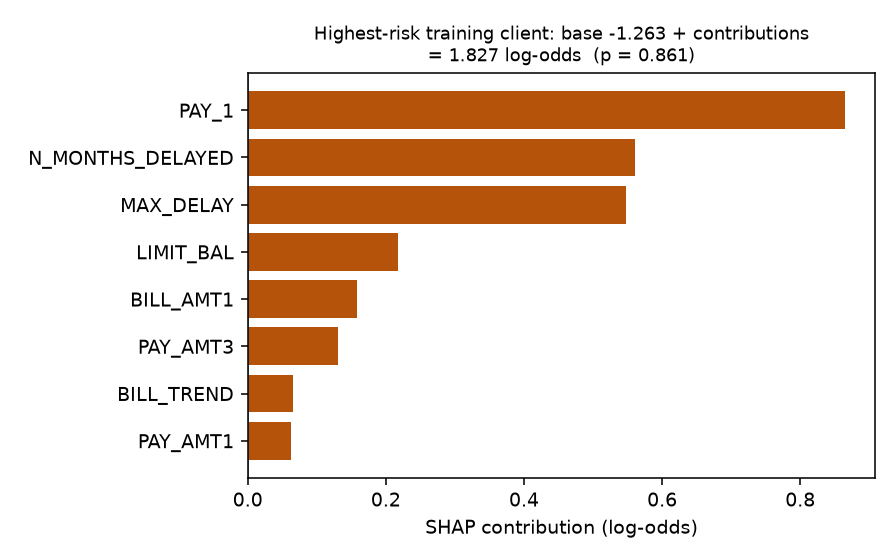
\includegraphics[width=0.92\linewidth]{shap_waterfall.png}
  \caption{One client decomposed: base value plus each feature's contribution.}
  \label{fig:shap-waterfall}
\end{figure}

\begin{figure}[p]
  \centering
  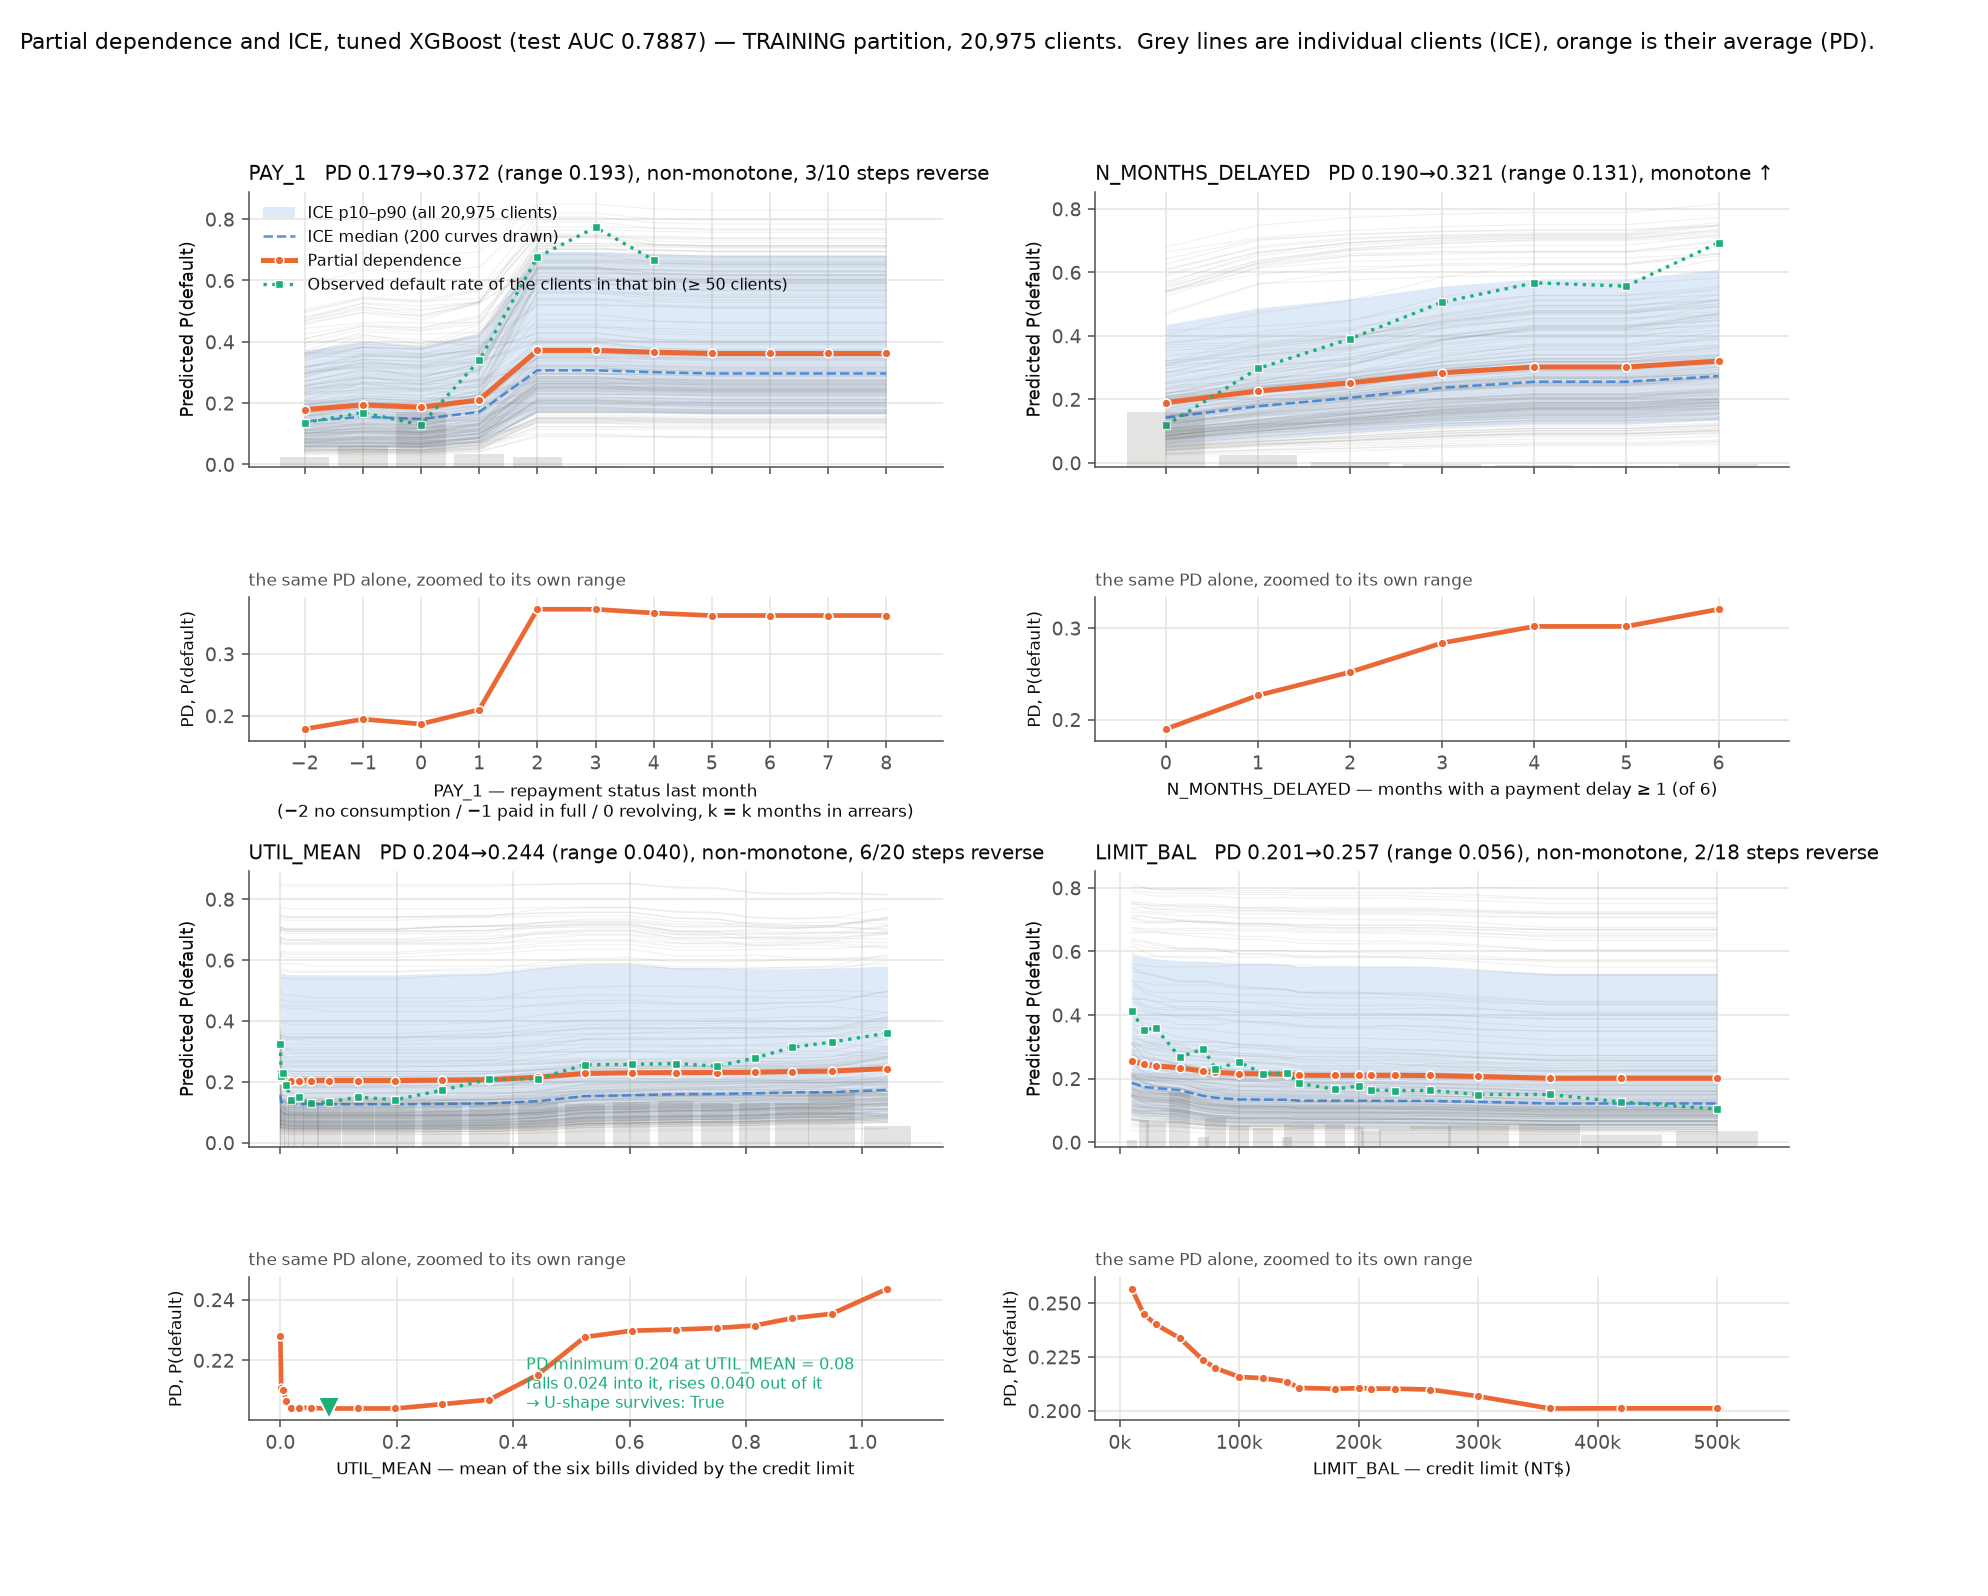
\includegraphics[width=1.0\linewidth]{pdp_main.png}
  \caption{Partial dependence with ICE curves for the four features that matter.}
  \label{fig:pdp-main}
\end{figure}

\begin{figure}[p]
  \centering
  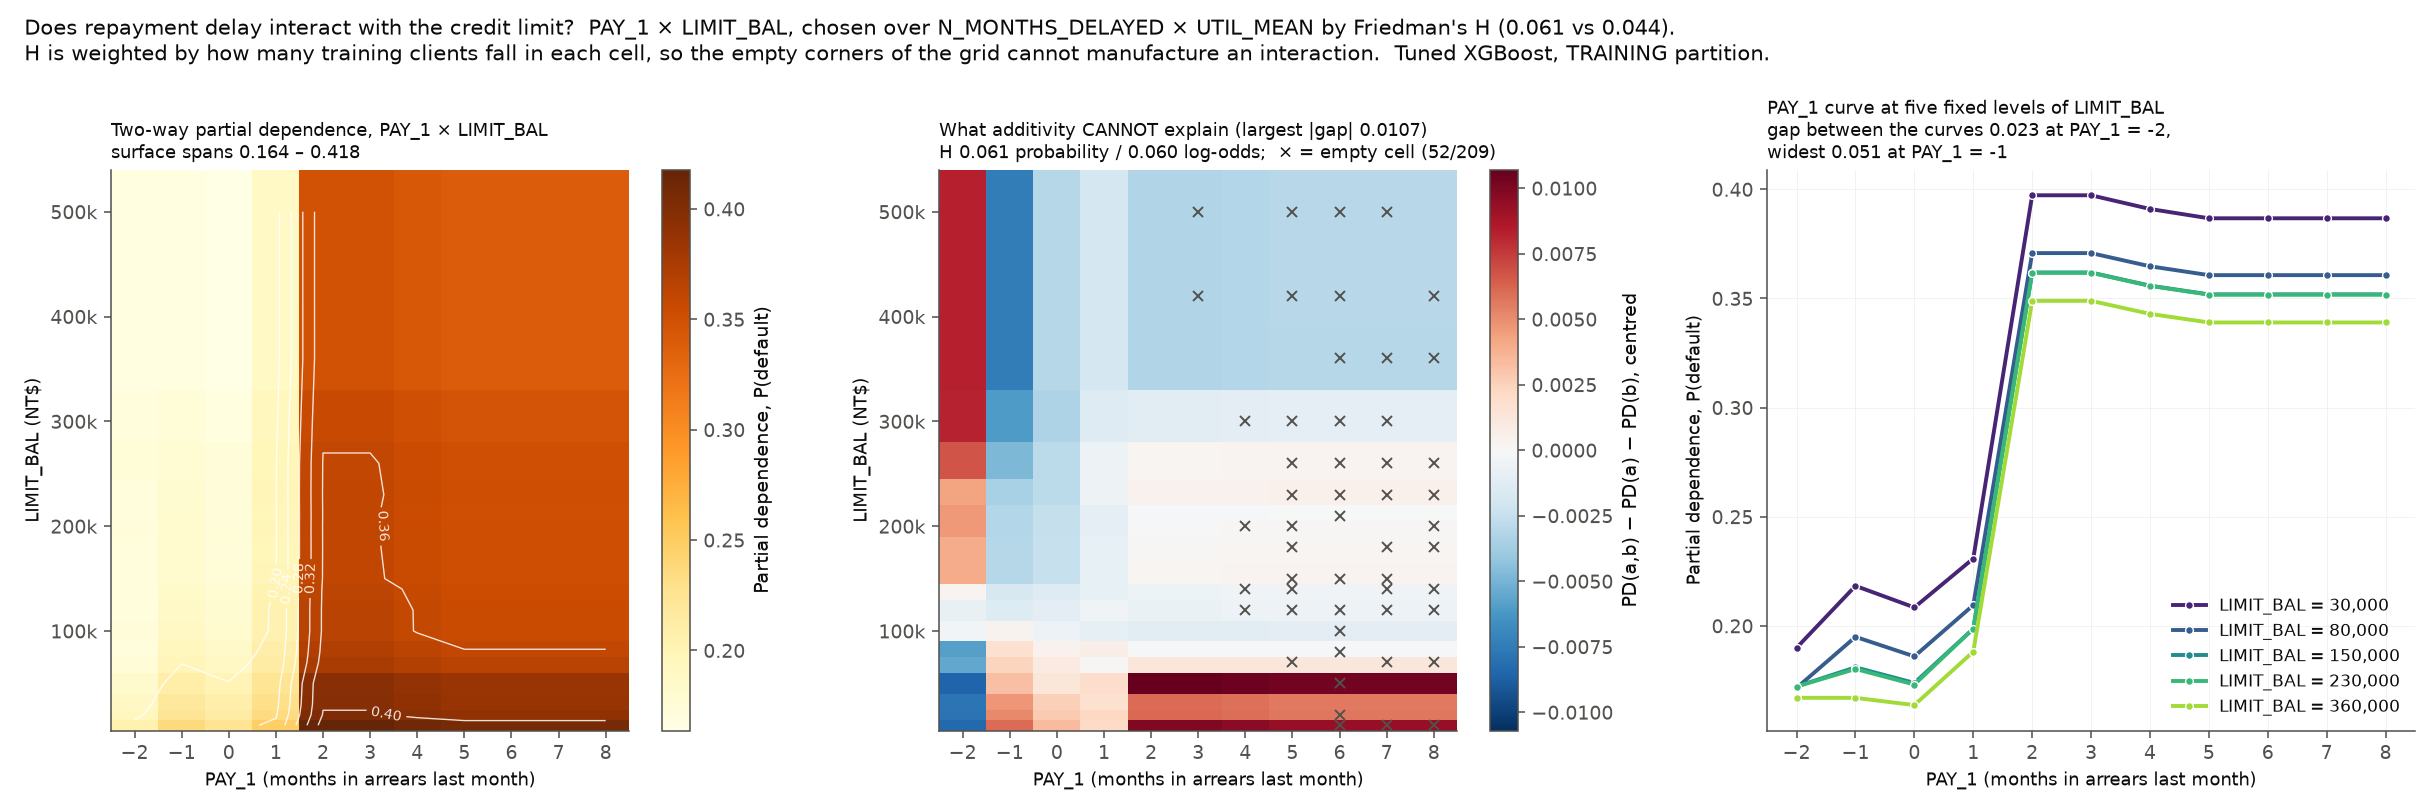
\includegraphics[width=1.0\linewidth]{pdp_interaction.png}
  \caption{Two-way partial dependence; cells with no training client are crossed.}
  \label{fig:pdp-interaction}
\end{figure}

\begin{figure}[htbp]
  \centering
  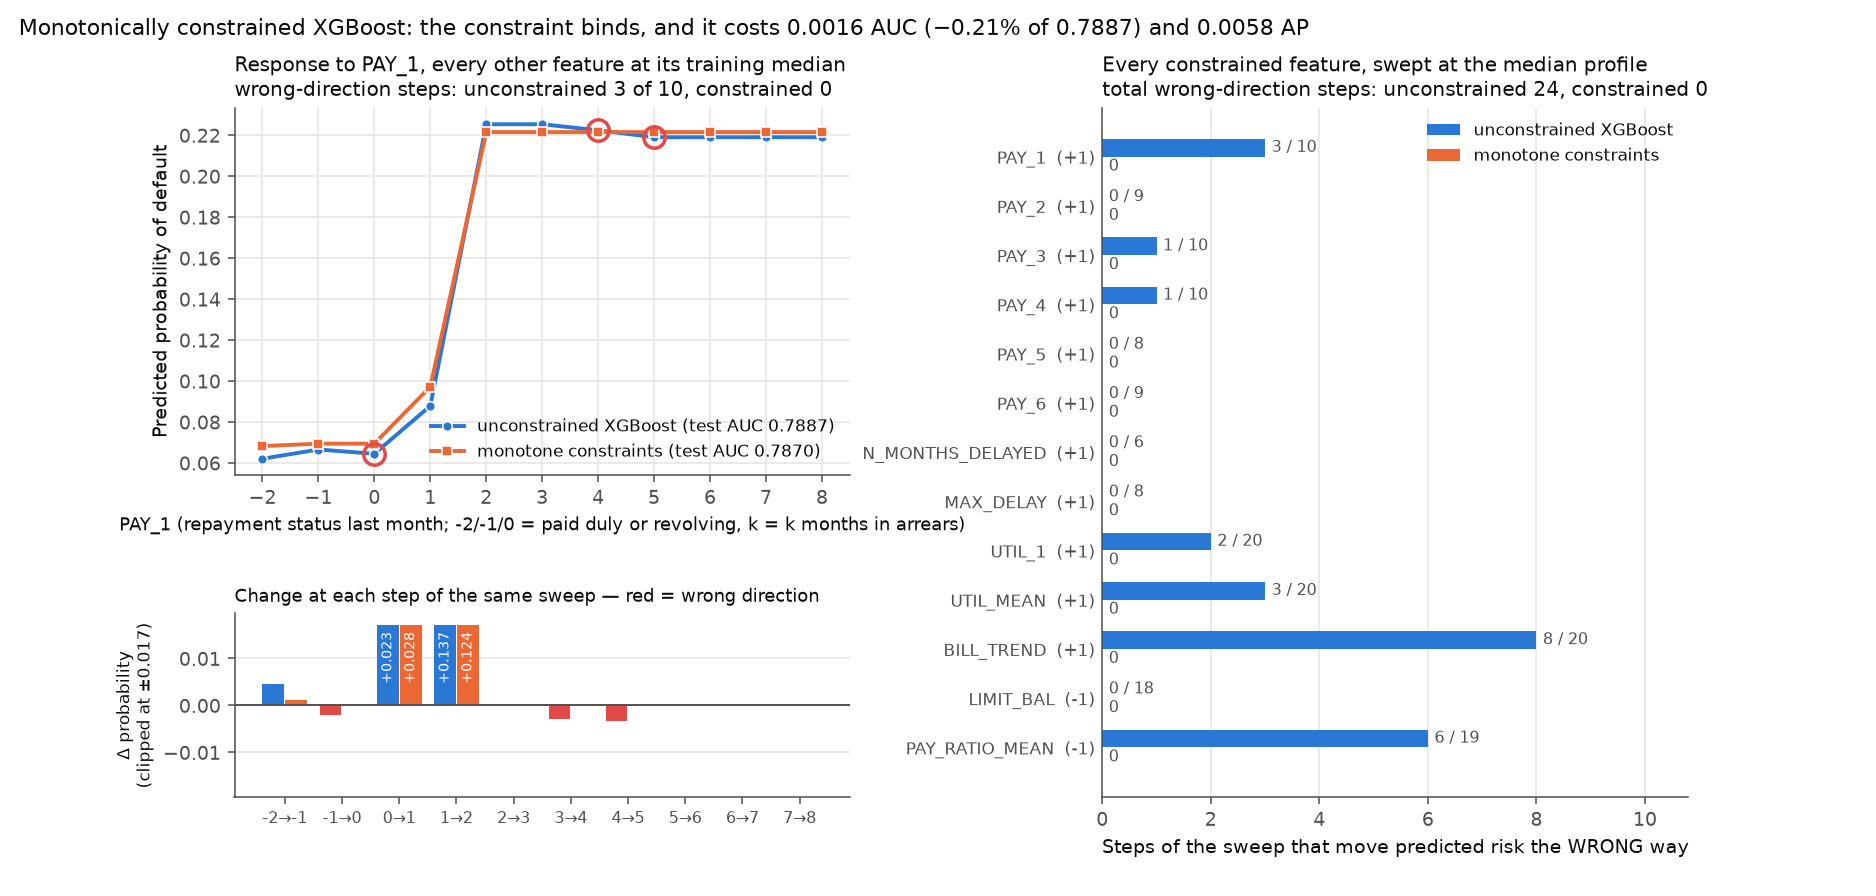
\includegraphics[width=0.92\linewidth]{monotone_pay1.png}
  \caption{Predicted probability against the most recent repayment status, with and without monotone constraints.}
  \label{fig:monotone-pay1}
\end{figure}

\begin{figure}[htbp]
  \centering
  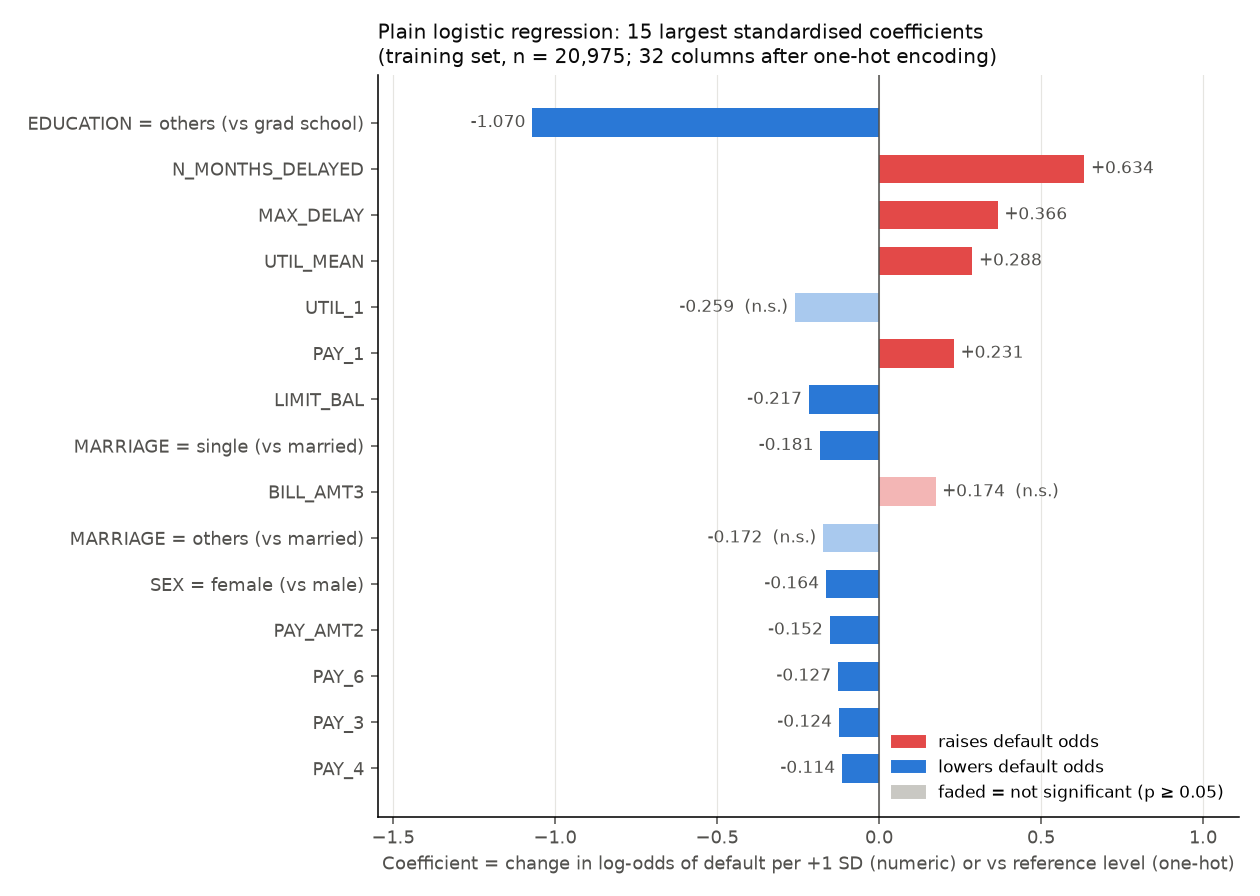
\includegraphics[width=0.92\linewidth]{logistic_coefficients.png}
  \caption{Standardised logistic coefficients.}
  \label{fig:logistic-coefficients}
\end{figure}
\clearpage

\begin{figure}[htbp]
  \centering
  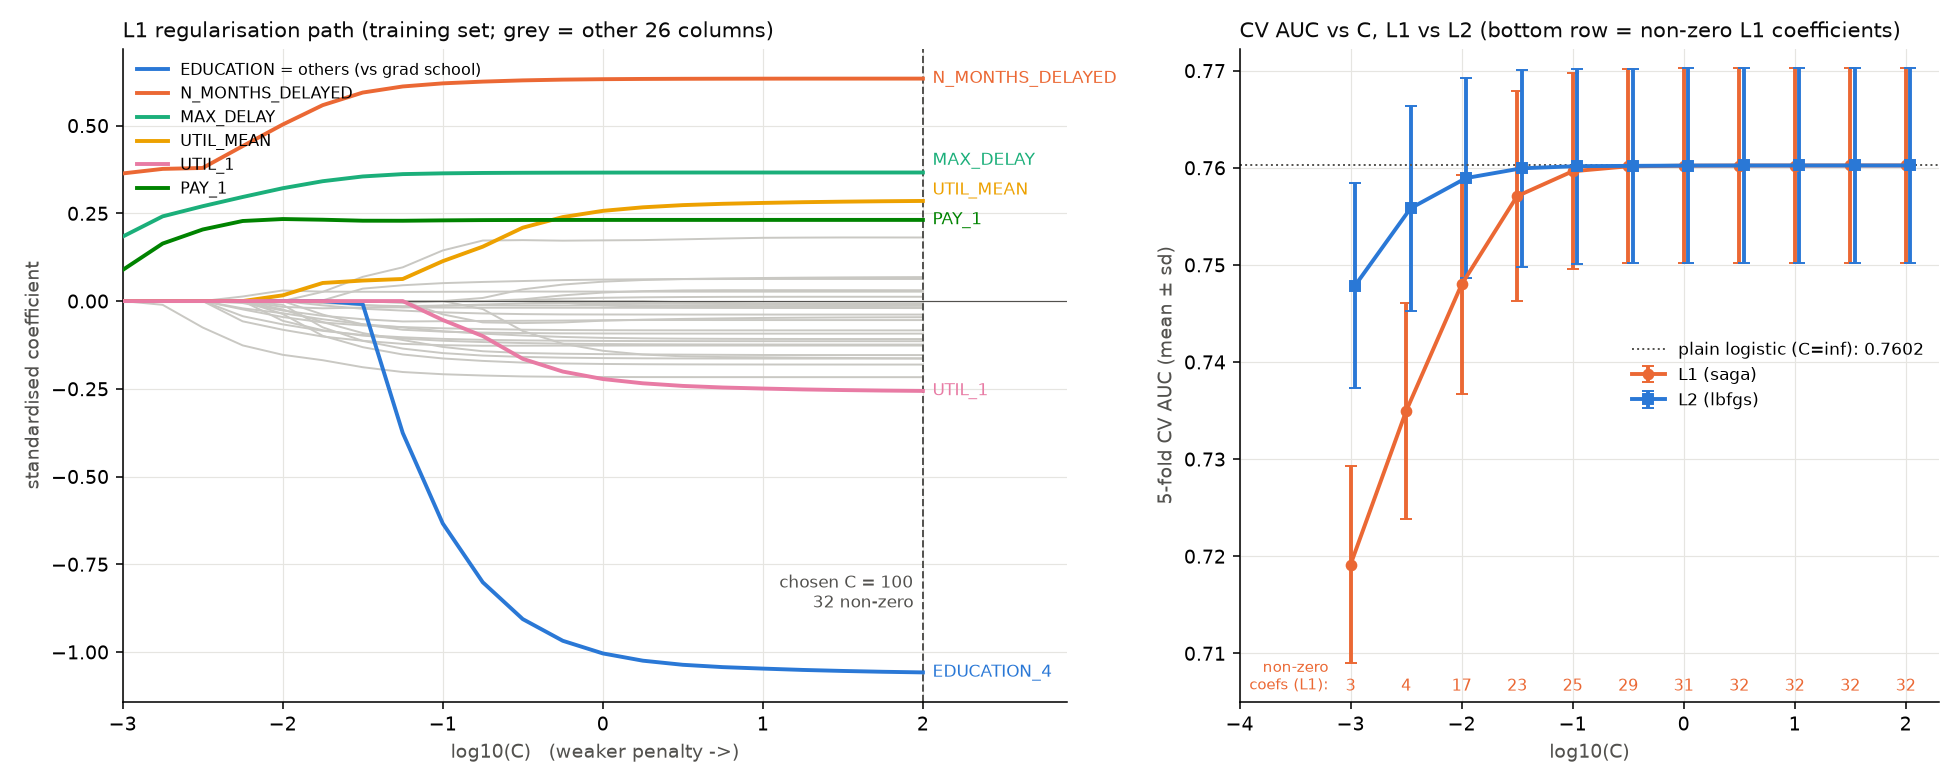
\includegraphics[width=0.92\linewidth]{logistic_l1_path.png}
  \caption{Lasso path: order of entry of the predictors as the penalty is relaxed.}
  \label{fig:logistic-l1-path}
\end{figure}

\begin{figure}[htbp]
  \centering
  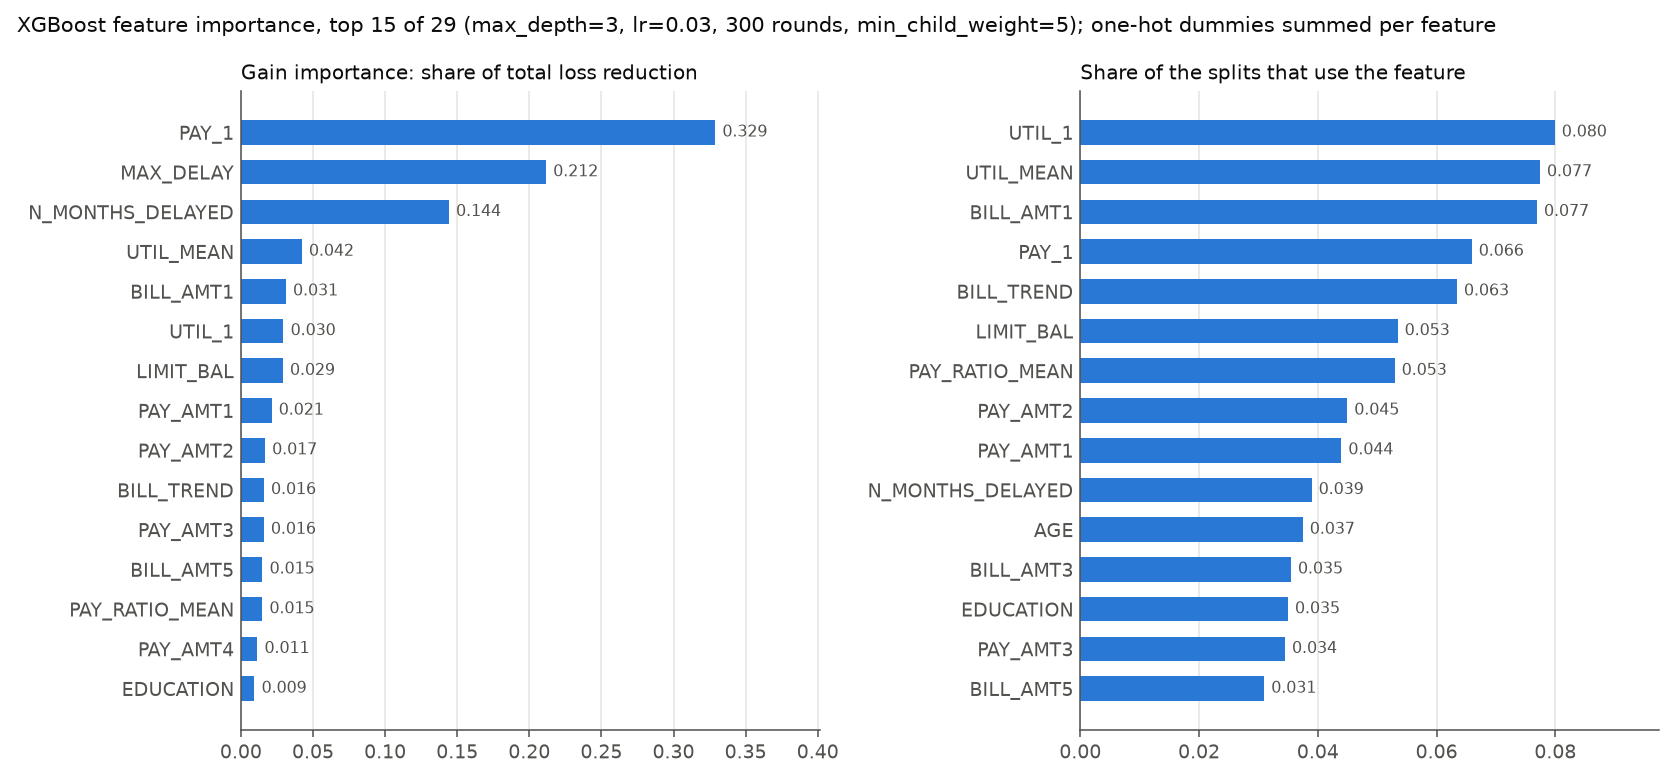
\includegraphics[width=0.92\linewidth]{xgb_importance.png}
  \caption{XGBoost gain-based importance.}
  \label{fig:xgb-importance}
\end{figure}

\begin{figure}[htbp]
  \centering
  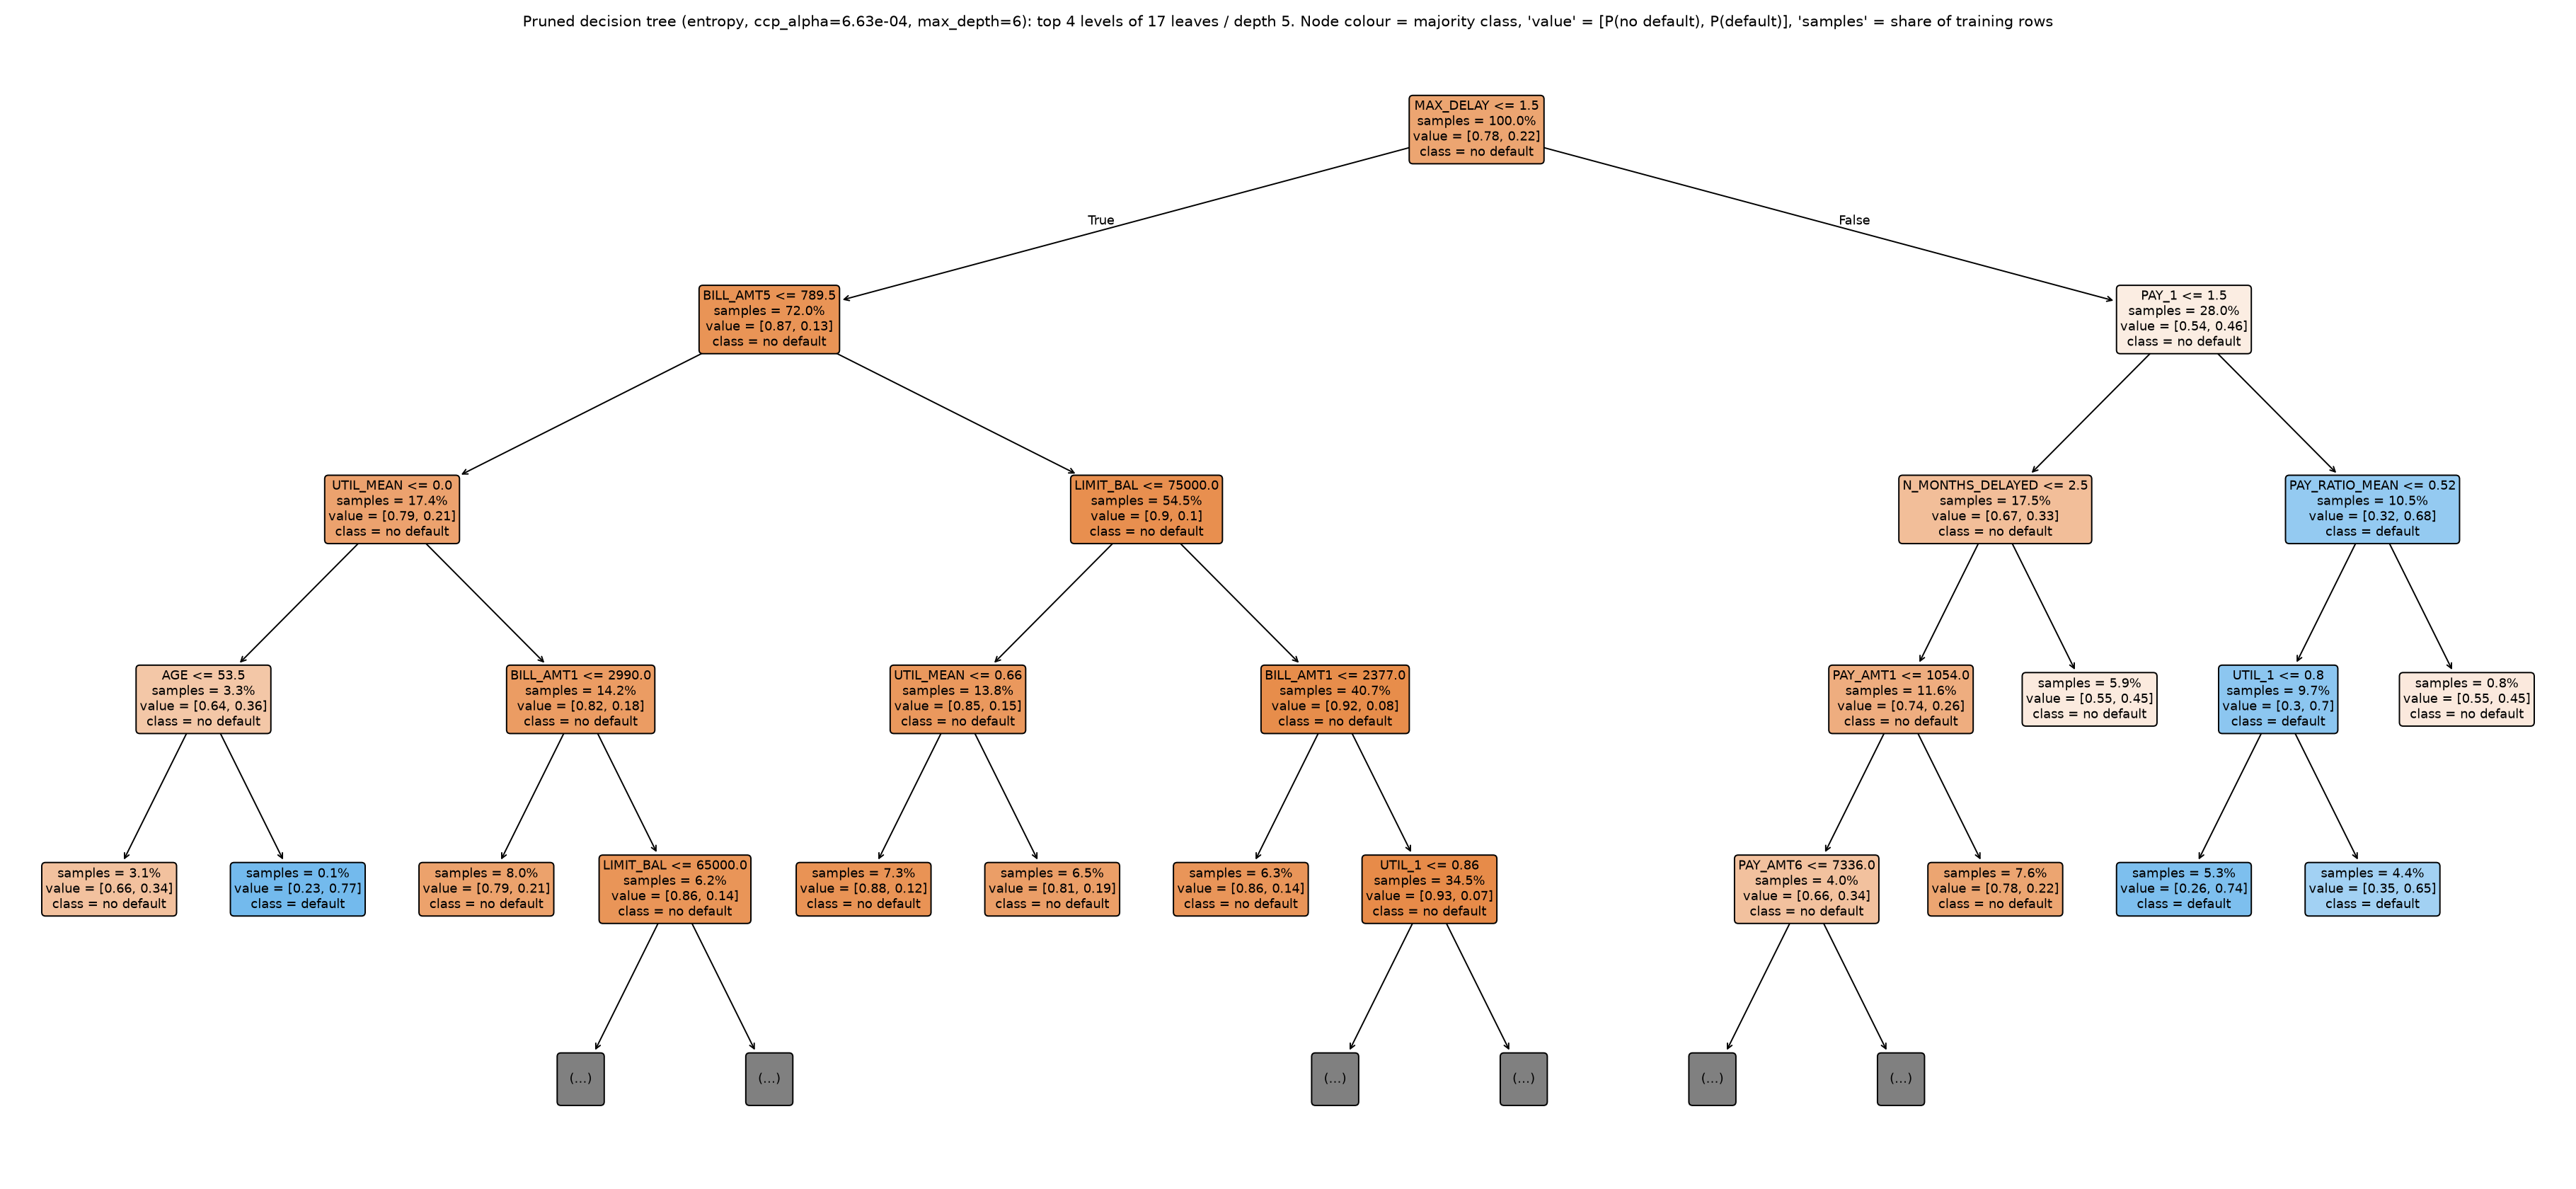
\includegraphics[width=0.92\linewidth]{tree_pruned.png}
  \caption{The pruned decision tree, top levels.}
  \label{fig:tree-pruned}
\end{figure}

\clearpage
\subsection{Class imbalance and the leakage demonstration}

\begin{figure}[htbp]
  \centering
  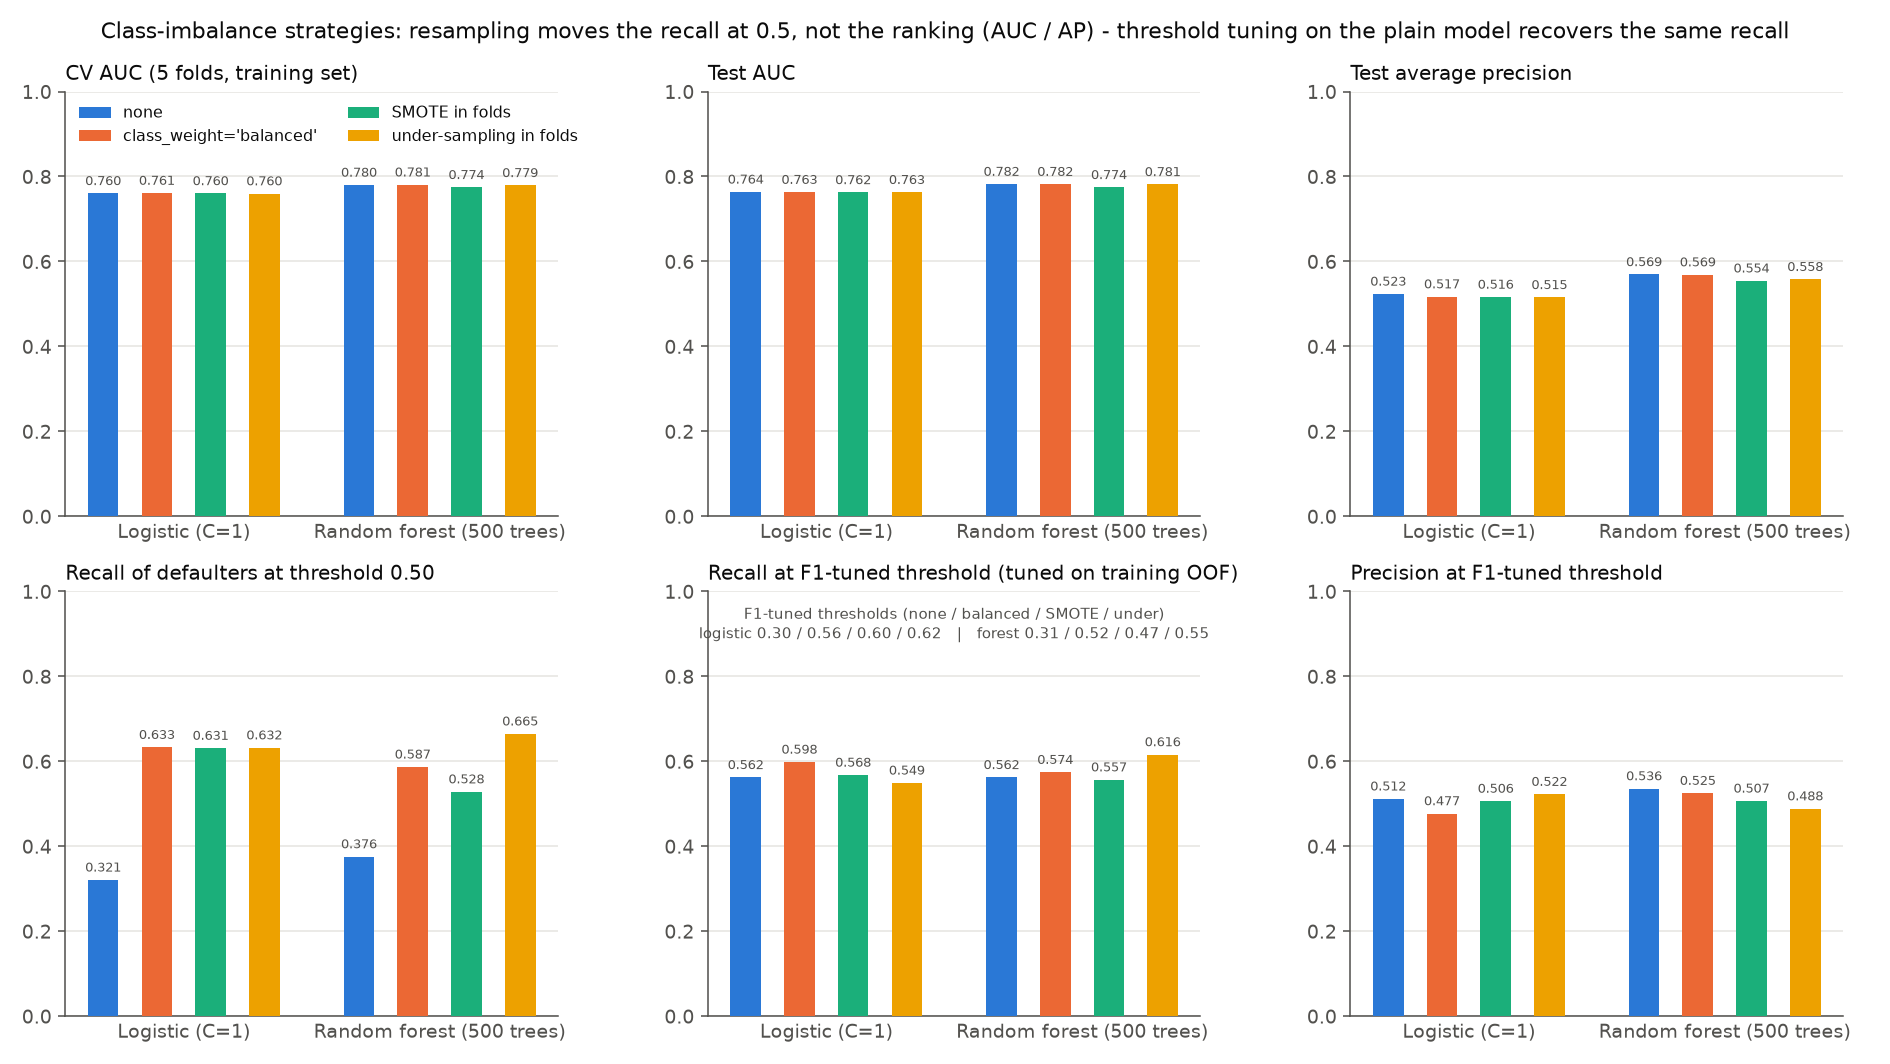
\includegraphics[width=0.92\linewidth]{imbalance_comparison.png}
  \caption{Resampling strategies applied inside the folds: AUC is unchanged, the operating point moves.}
  \label{fig:imbalance-comparison}
\end{figure}

\begin{figure}[htbp]
  \centering
  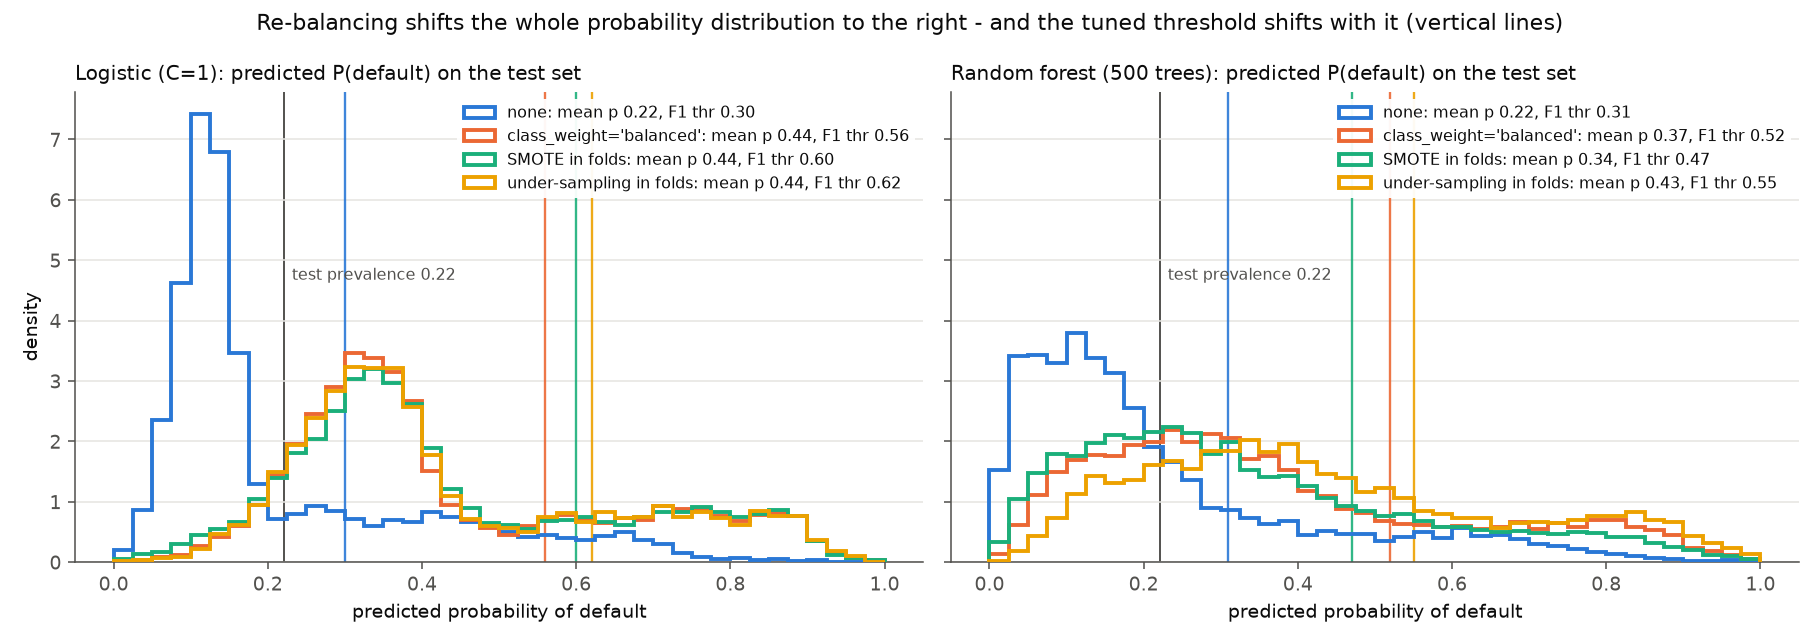
\includegraphics[width=0.92\linewidth]{imbalance_threshold_shift.png}
  \caption{Where each resampling strategy puts the tuned threshold.}
  \label{fig:imbalance-threshold-shift}
\end{figure}

\begin{figure}[htbp]
  \centering
  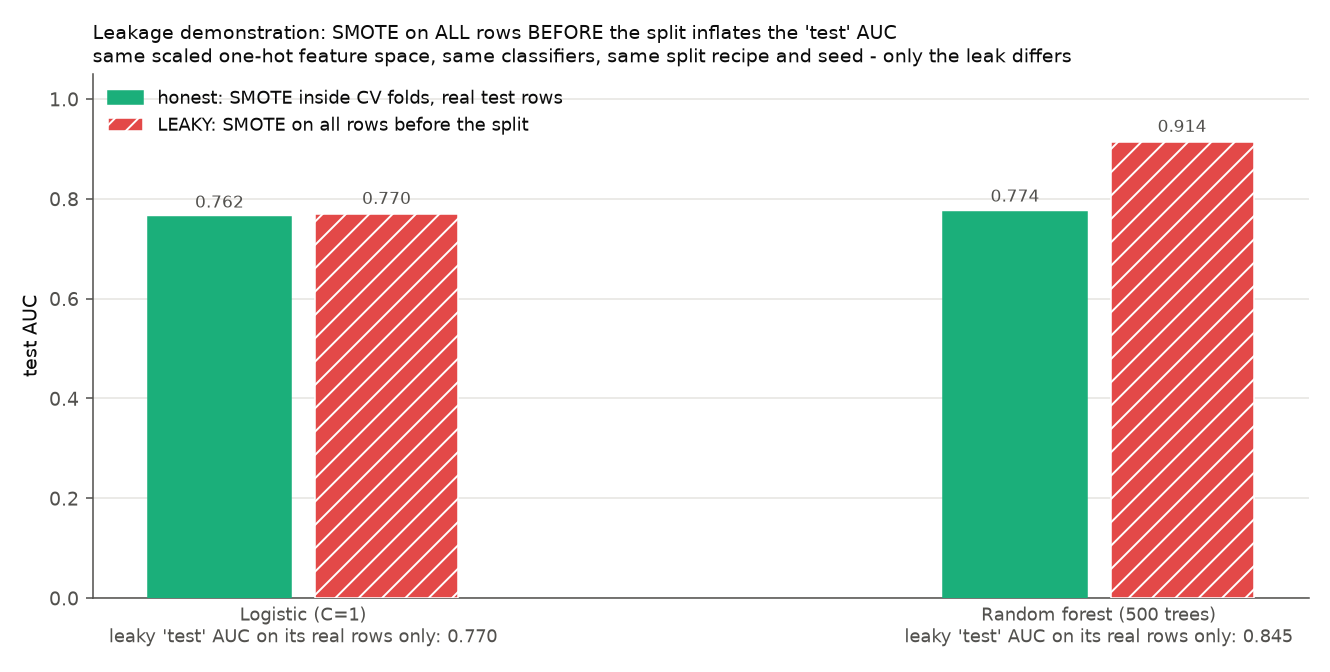
\includegraphics[width=0.92\linewidth]{imbalance_leakage_demo.png}
  \caption{Negative control: SMOTE applied before the split inflates the apparent test AUC.}
  \label{fig:imbalance-leakage-demo}
\end{figure}
\clearpage

\clearpage
\subsection{Model selection diagnostics}

\begin{figure}[htbp]
  \centering
  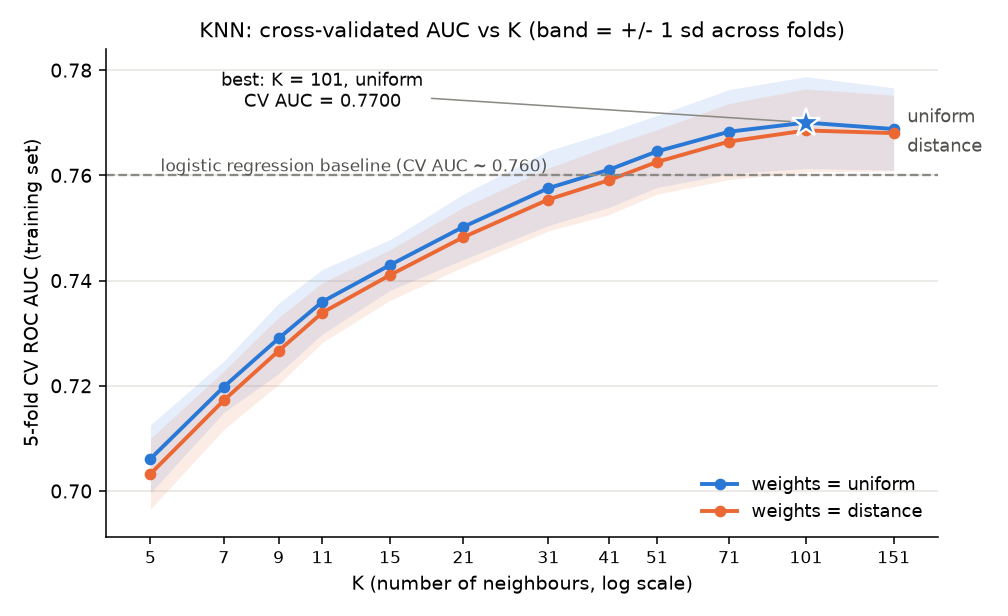
\includegraphics[width=0.92\linewidth]{knn_cv_auc_vs_k.png}
  \caption{KNN: cross-validated AUC against $K$.}
  \label{fig:knn-cv-auc-vs-k}
\end{figure}

\begin{figure}[htbp]
  \centering
  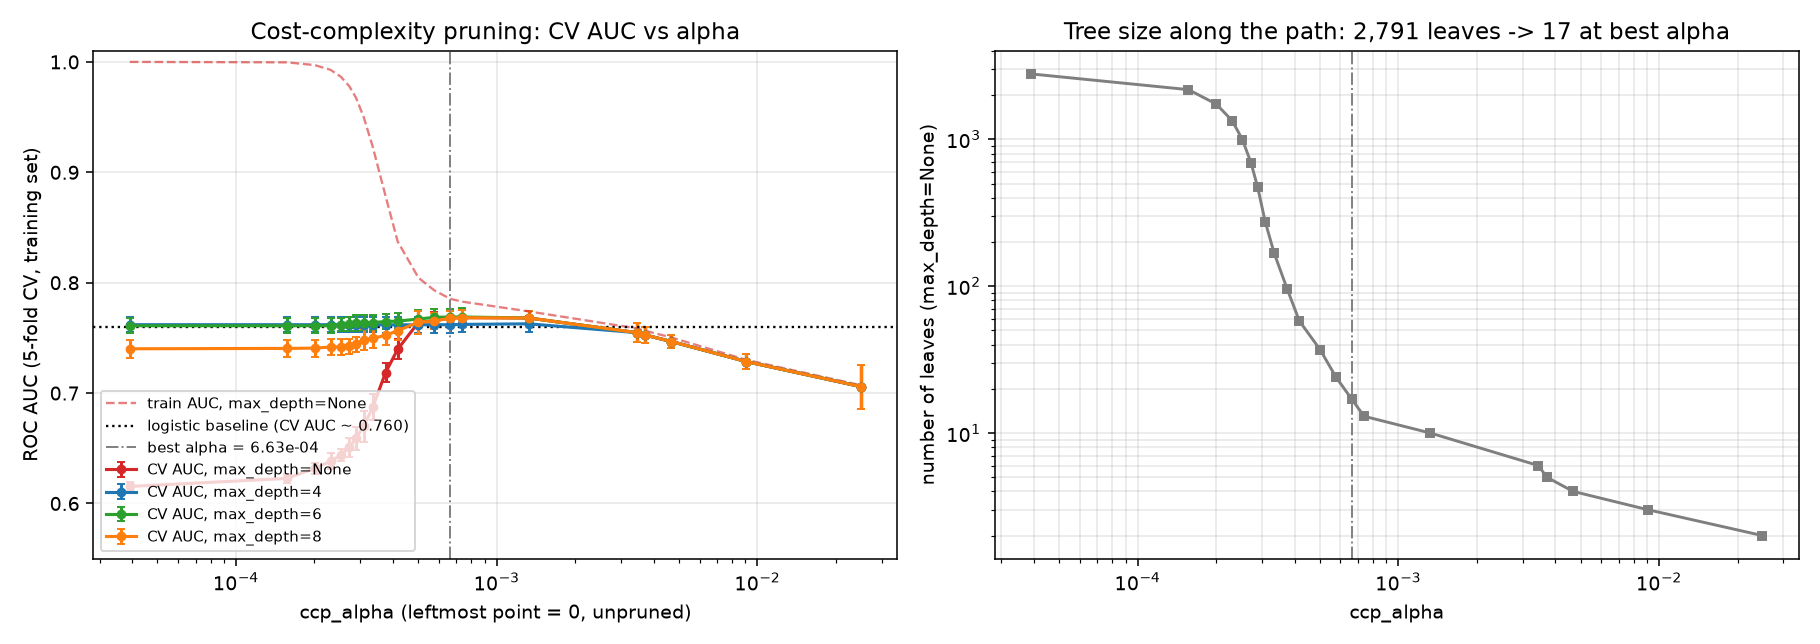
\includegraphics[width=0.92\linewidth]{tree_cv_auc_vs_alpha.png}
  \caption{Cost-complexity pruning path.}
  \label{fig:tree-cv-auc-vs-alpha}
\end{figure}

\begin{figure}[htbp]
  \centering
  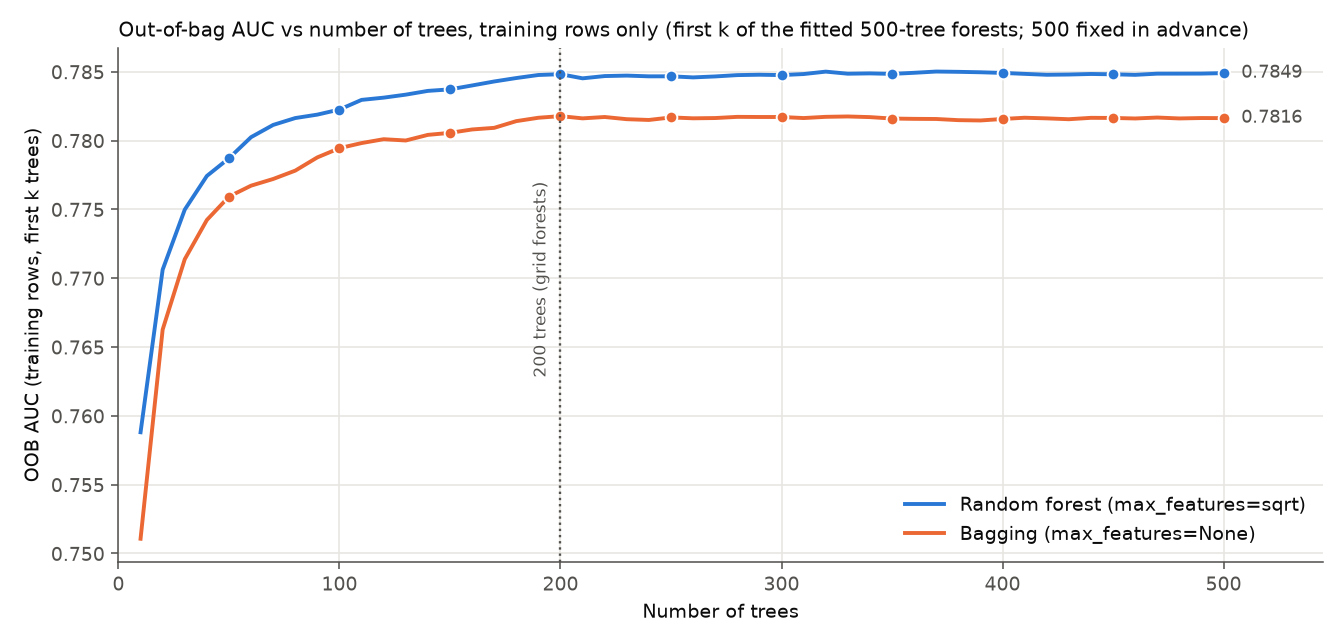
\includegraphics[width=0.92\linewidth]{rf_auc_vs_ntrees.png}
  \caption{Random forest: out-of-bag and test AUC against the number of trees.}
  \label{fig:rf-auc-vs-ntrees}
\end{figure}

\begin{figure}[htbp]
  \centering
  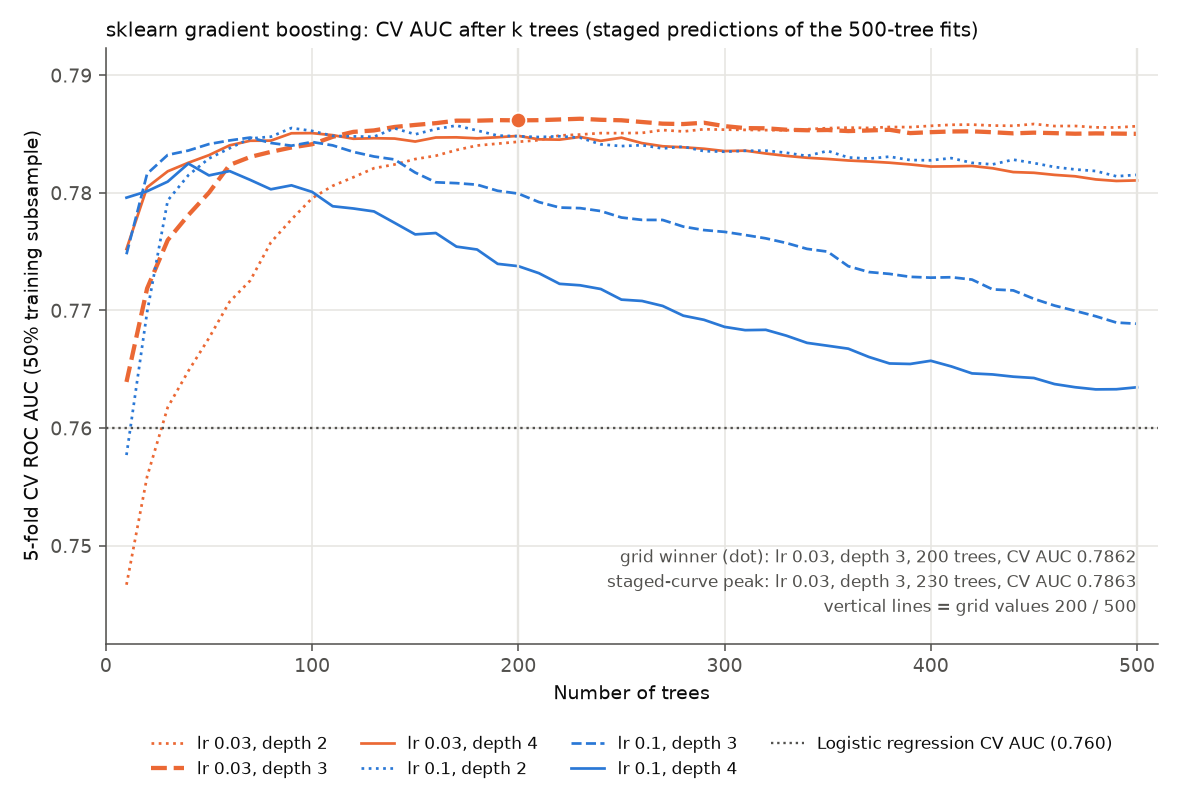
\includegraphics[width=0.92\linewidth]{gbm_learning_curve.png}
  \caption{Gradient boosting: cross-validated AUC against the number of rounds.}
  \label{fig:gbm-learning-curve}
\end{figure}

\begin{figure}[htbp]
  \centering
  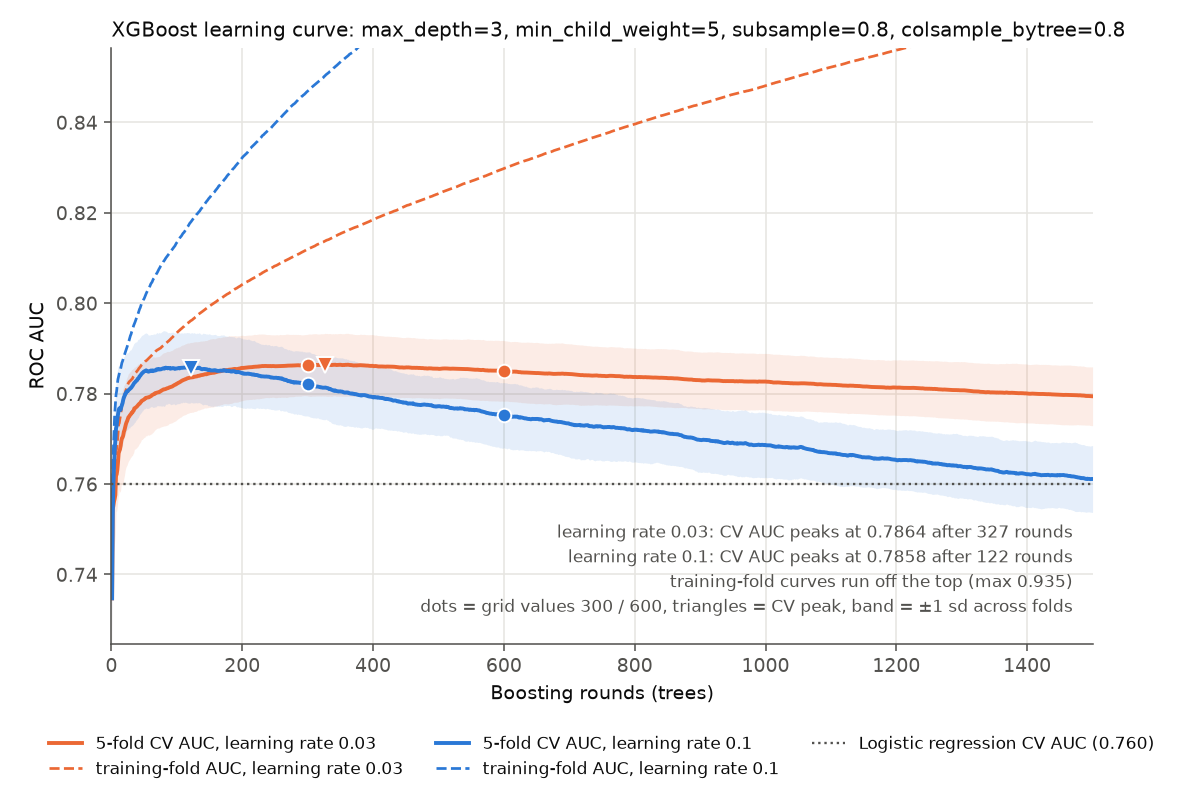
\includegraphics[width=0.92\linewidth]{xgb_learning_curve.png}
  \caption{XGBoost learning curves at two learning rates.}
  \label{fig:xgb-learning-curve}
\end{figure}

\begin{figure}[htbp]
  \centering
  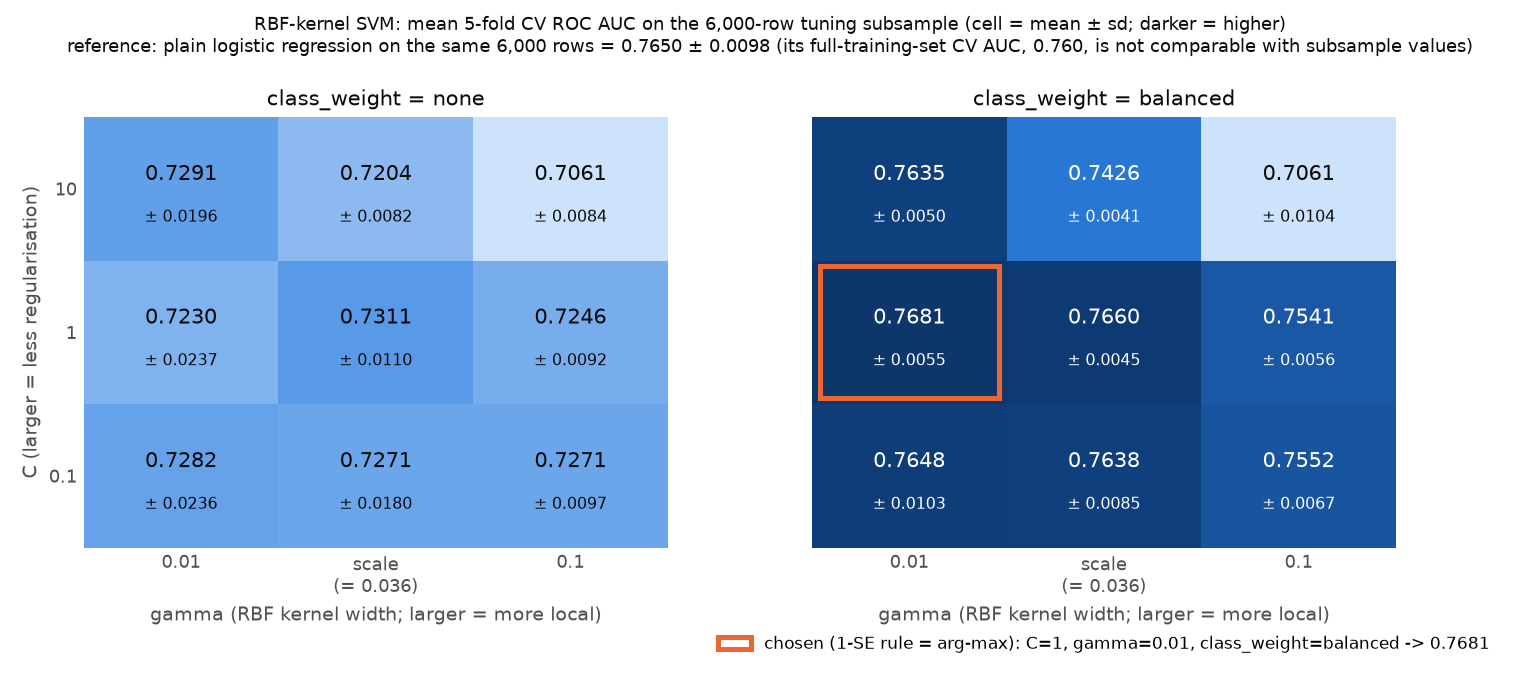
\includegraphics[width=0.92\linewidth]{svm_rbf_cv_heatmap.png}
  \caption{RBF support-vector machine: cross-validated AUC over $C$ and $\gamma$.}
  \label{fig:svm-rbf-cv-heatmap}
\end{figure}
\clearpage

\begin{figure}[htbp]
  \centering
  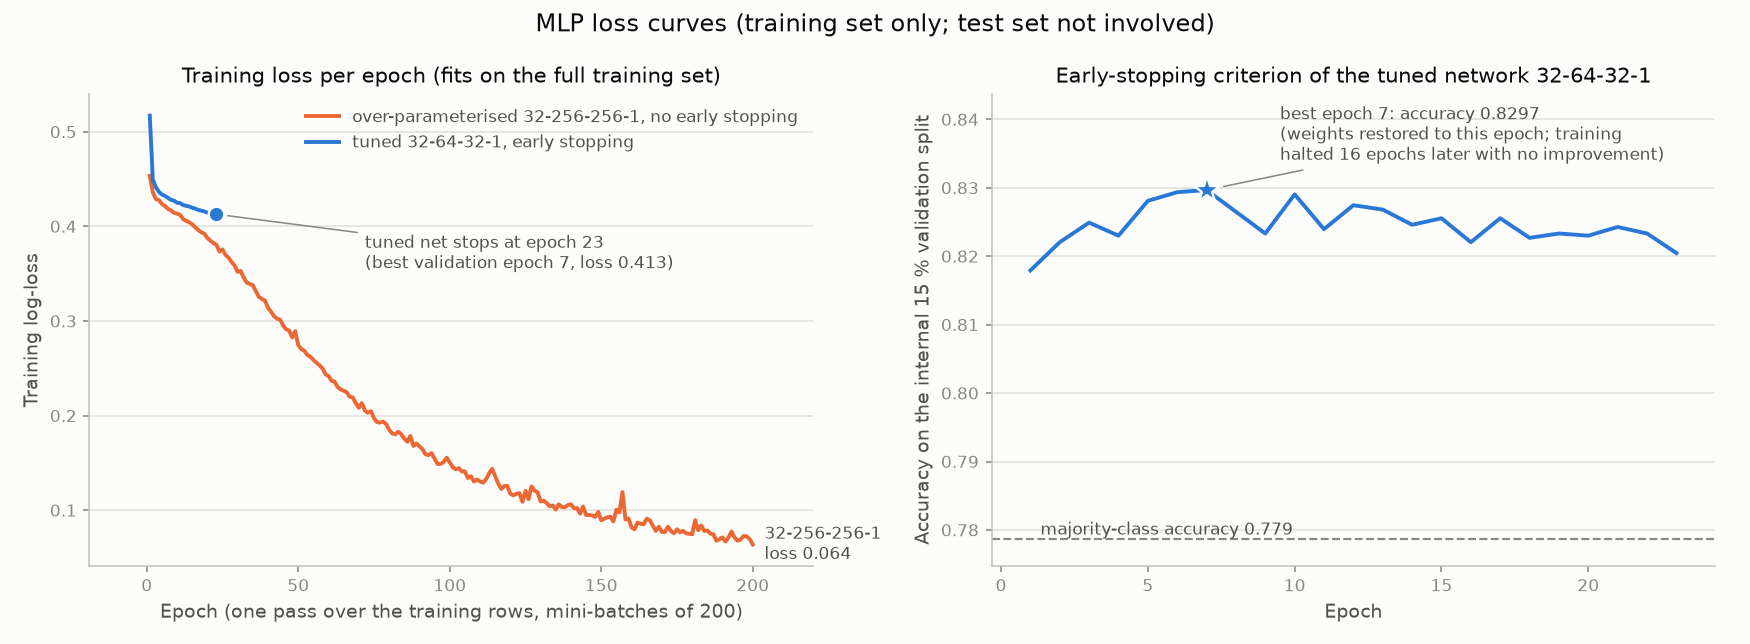
\includegraphics[width=0.92\linewidth]{mlp_loss_curve.png}
  \caption{Neural network: training loss and validation AUC by epoch.}
  \label{fig:mlp-loss-curve}
\end{figure}

\begin{figure}[htbp]
  \centering
  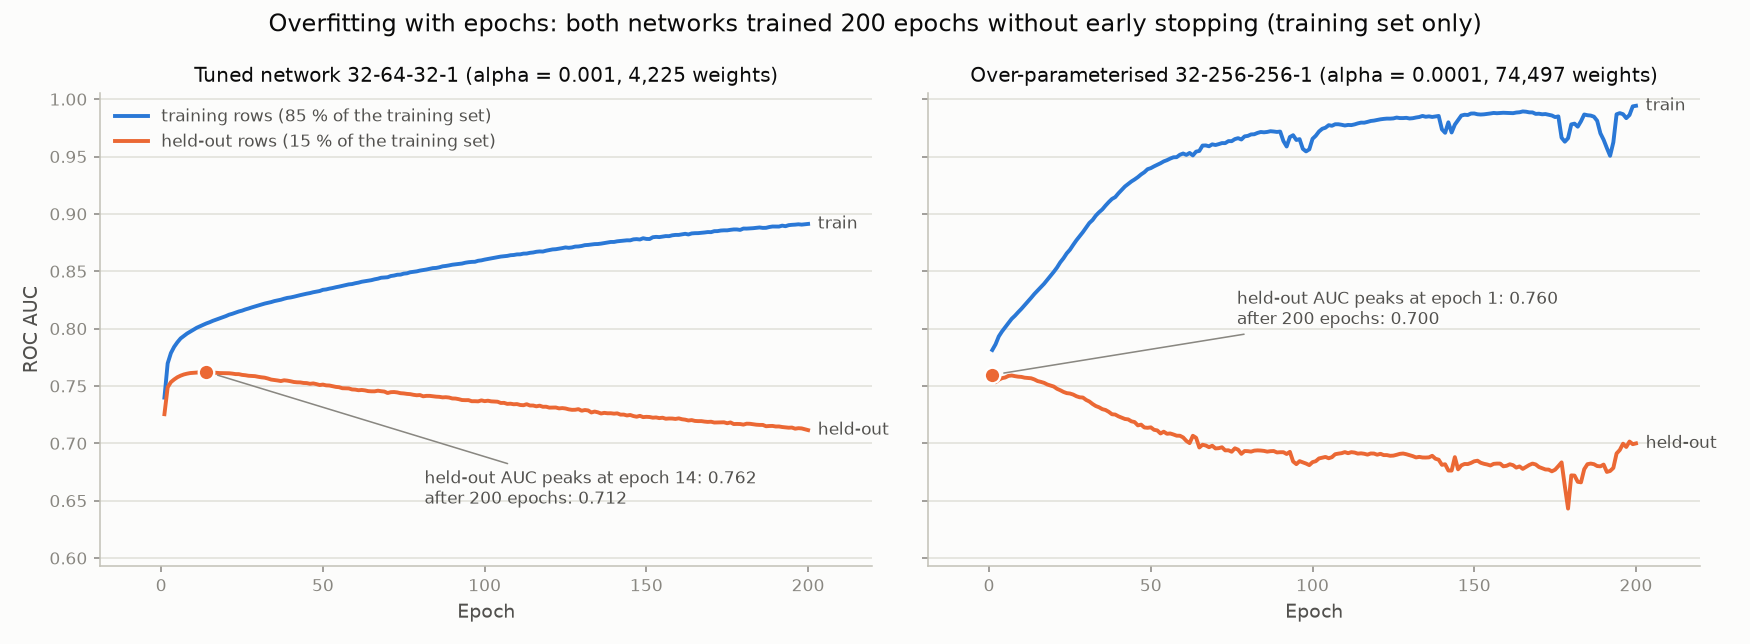
\includegraphics[width=0.92\linewidth]{mlp_overfit_epochs.png}
  \caption{Over-parameterised network: the over-fitting diagnostic.}
  \label{fig:mlp-overfit-epochs}
\end{figure}

\begin{figure}[htbp]
  \centering
  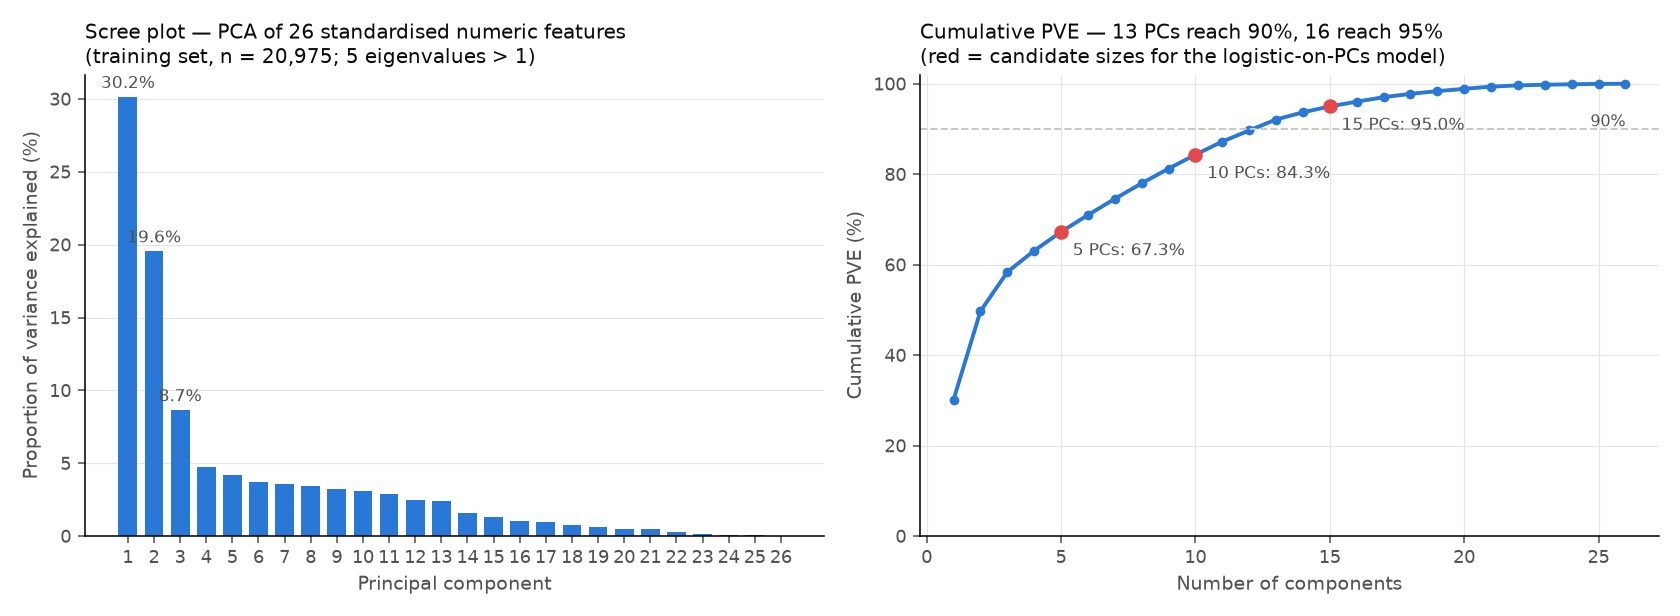
\includegraphics[width=0.92\linewidth]{pca_scree.png}
  \caption{PCA scree plot and cumulative variance explained.}
  \label{fig:pca-scree}
\end{figure}

\begin{figure}[p]
  \centering
  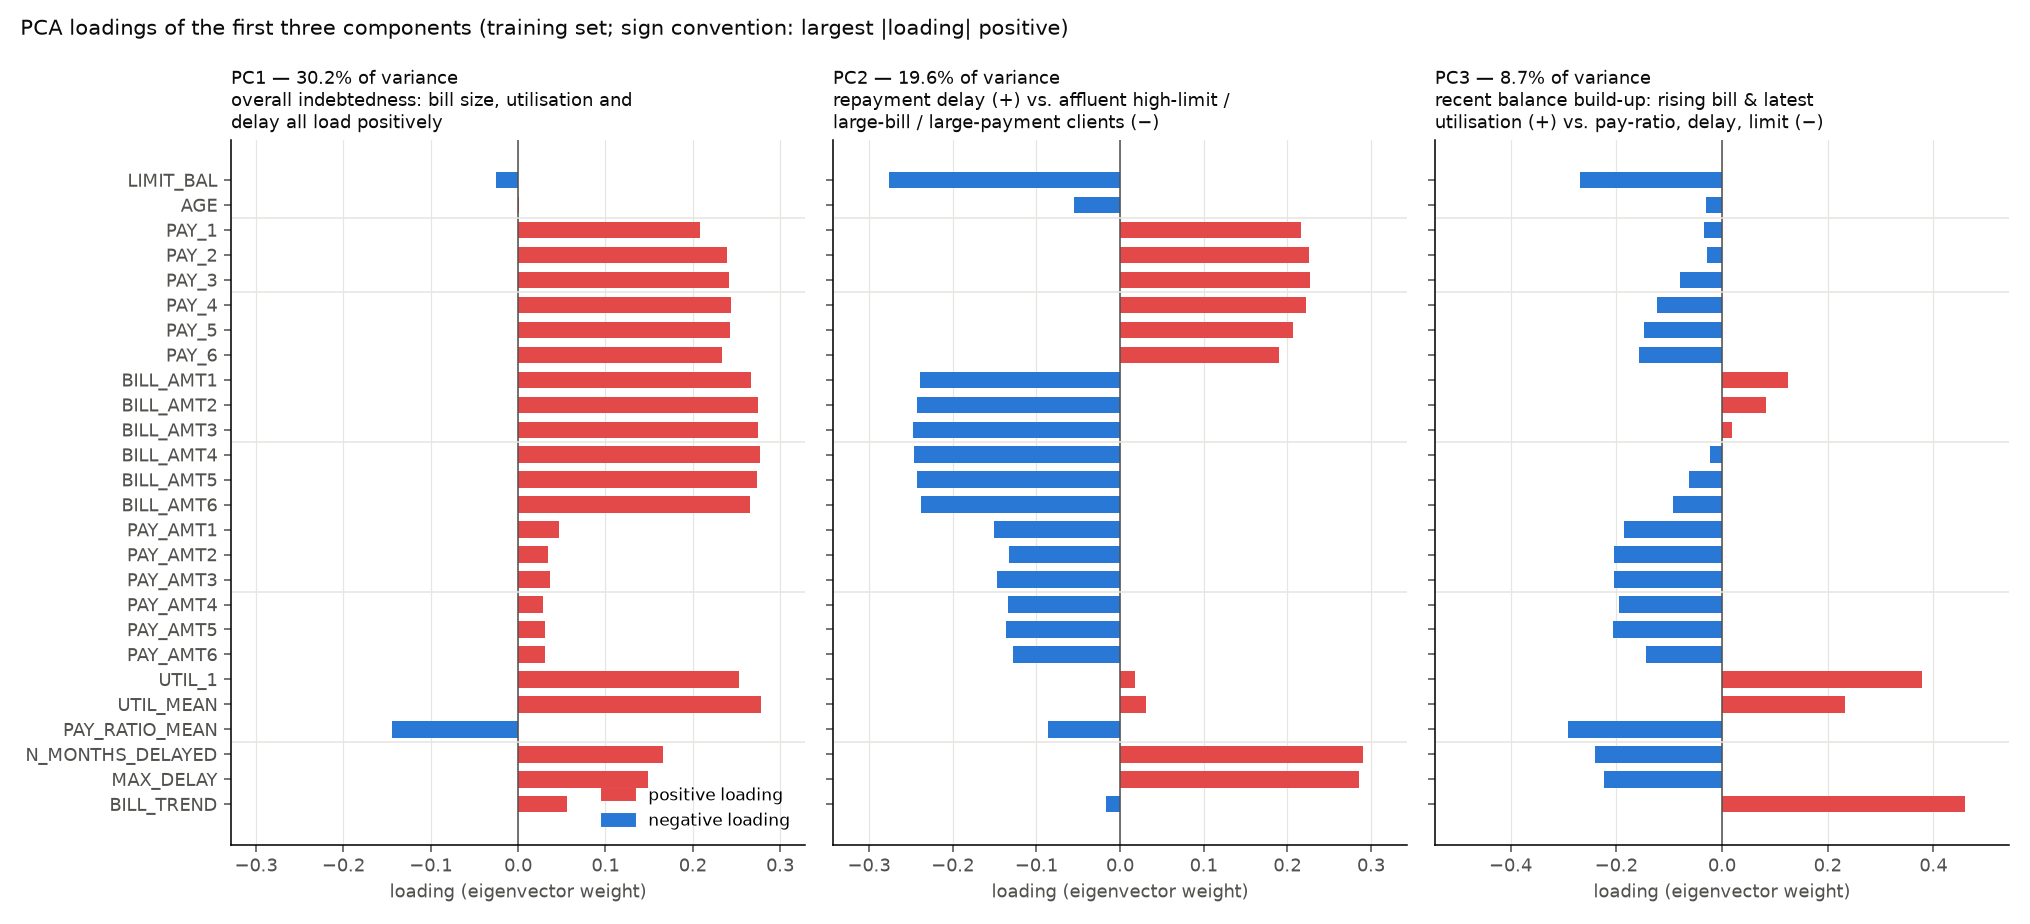
\includegraphics[width=1.0\linewidth]{pca_loadings.png}
  \caption{Loadings of the first three principal components.}
  \label{fig:pca-loadings}
\end{figure}

\begin{figure}[htbp]
  \centering
  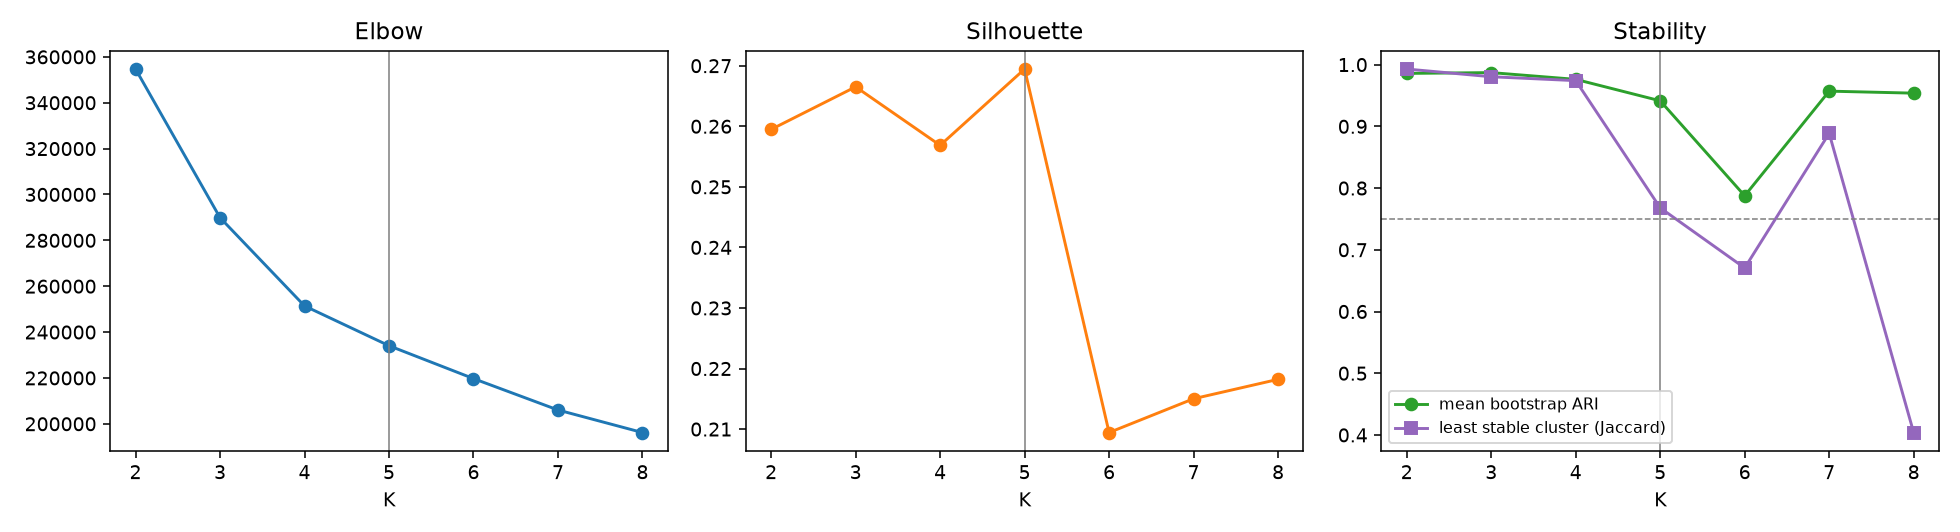
\includegraphics[width=0.92\linewidth]{kmeans_selection_repro.png}
  \caption{K-means on the first 10 principal components: silhouette, bootstrap ARI and minimum cluster Jaccard against $K$ (Table~\ref{tab:a-kselect}); reproduction on 21 October of RUAN Hangjing's 30 September analysis, training partition only.}
  \label{fig:kmeans-selection-repro}
\end{figure}

